\documentclass[a4paper,12pt]{article}
\usepackage[hidelinks]{hyperref}
\usepackage{float}
\usepackage{amsmath}
\usepackage{tcolorbox}
\usepackage{amsmath, amssymb, tikz}
\usepackage{hyperref}
\usepackage[utf8]{inputenc}
\usepackage[vietnamese, english]{babel} 
\usepackage{amsmath, amssymb}
\usepackage{geometry}
\geometry{a4paper, margin=1in}
\usepackage{tocloft}
\usepackage{float} 
\usepackage{xcolor}
\usepackage{titlesec}
\renewcommand{\cftsecfont}{\bfseries}
\usepackage{graphicx}
\usepackage{setspace}
\usepackage{titlesec}
\usepackage{pgfplots}
\titleformat{\section}[block]{\Large\bfseries}{\thesection}{1em}{}
\makeatletter
\renewcommand*\env@matrix[1][*\c@MaxMatrixCols c]{%
  \hskip -\arraycolsep
  \let\@ifnextchar\new@ifnextchar
  \array{#1}}
\makeatother
% Hien thi LOGO HUS
\begin{titlepage}
\begin{center}

\textbf{\LARGE  Vietnam National University, Hanoi\\Hanoi University of Science\\}
\end{center}

\begin{figure}[h!]
\begin{center}
\includegraphics[width=4cm]{Images/LOGO_HUS.png}
\end{center}
\end{figure}

\begin{center}
\begin{tabular}{c}
\multicolumn{1}{c}{\textbf{{\LARGE ENGLISH FOR CIS - K68A3 CIS}}}\\
~~\\
\\
\hline
\\

\textbf{{\Large Final Report: Linear Algebra}}\\
\\
\hline
\end{tabular}
\end{center}

\vspace{2cm}

\begin{table}[h]
\begin{tabular}{rrll}

\hspace{5 cm}

\textbf{Report conducted by:} \\
\\

\textbf{Full Name} & &\textbf{Student ID}\\
Nguyen Tran Phuc Chau & & 23001835 \\
Bui Quang Chien & & 23001837 \\
Nguyen Le Ngoc Bao & & 23001832 \\

\end{tabular}
\end{table}

\vspace{3cm}

\begin{center}
{\footnotesize Hanoi, December, 2024}
\end{center}
\end{titlepage}
\begin{document}
% Introduction Section
\section*{Introduction}
The purpose of this report is to summarize the work of Group 5, which consists of three members who are the authors of this report. Due to the limited time available and the practical focus of the project, this report is not intended to serve as an educational resource or as an academically rigorous document. Rather, it provides sufficient knowledge and explanations, though there may still be some gaps. We welcome feedback from readers to help improve the quality of this report.

The authors thank the readers for taking the time to read this report.

Sincerely 
\begin{flushright}
Signed

Chau

Nguyen Tran Phuc Chau
\end{flushright}

\newpage
\setcounter{tocdepth}{3}
\tableofcontents 
\newpage


\Large \section{System of Linear Equation: Algebra}
\small The objective of this content is to introduce the definitions of a linear equation system, to solve a linear equation system and to present the solutions using the \textbf{parametric form}.
\Large \subsection{System of  Linear Equation}
    \begin{frame}
        \small
        
        \small To begin, it is essential to develop a clear understanding of what a \textbf{ system of linear equations} entails and the principles underlying its structure. Furthermore, we must dive into the various methods and techniques used to solve such systems effectively, ranging from traditional substitution and elimination methods to more advanced approaches like matrix operations and \textbf{Gaussian elimination} (This will be covered later on in section 1.2.1). This foundational knowledge serves as the foundation for the tackling of more complex problems and applications in mathematics and beyond.
        \small An \textbf{ equation} in the unknown \(x\), \(y\), \(z\),\dots is called \textbf{linear} if both sides of the equation are the sum of (constant) multiples of \(x\), \(y\), \(z\),\dots plus an optional constant.

        
        \subparagraph{Example 1:} 2\(x\) + \(y\) = 12, 3\(x\) + 6\(y\) = 2\(z\), \dots\\

        
        A \textbf{System of Linear Equation} is a collection of some several linear equations.


        \subparagraph{Example 2:}
        \begin{center}
            % Hệ phương trình ở giữa trang
            \begin{equation}
            \begin{cases}
                x + y = 3, \\
                2x - y = 4.
            \end{cases}
            \end{equation}
        \end{center}

        The \textbf{Solution:} of the system of linear equation is the values of \(x\), \(y\), \(z\),\dots that simultaneously satisfy all the equations in the system. The \textbf{solution set} is the collection of all solutions.\\

        \textbf{Solving} the system of linear equation means finding the solution set of it.\\

        We can easily prove that the solution set of a system of linear equation can have 1, infinite or 0 solution. The system which has no solution is called \textbf{inconsistent}, and be called \textbf{consistent} otherwise.

        
        
    \end{frame}

\Large \subsubsection{Line, Plane, Space, Etc}
    \begin{frame}
        \small 
        
        \small We use \textbf{R} to denote the set of all real number,i.e, the number line.

        \begin{tcolorbox}[title=Definition,colframe=blue!70!black, colback=blue!5!white]
        Let n be a positive whole number. We define:
        \begin{center}
            % Hệ phương trình ở giữa trang
            \small \( \mathbb{R}^{n} \) = all ordered n-tuples of real numbers(\(x_1\), \(x_2\), \(x_3\), \dots , \(x_n\))
        \end{center}
        \end{tcolorbox}
        \newpage
    \begin{figure}[H]
        \centering
        \includegraphics[width=1\linewidth]{Images/R1.png}
        \caption{The shape of \( \mathbb{R}^1 \).}
        \label{fig:enter-label}
    \end{figure}
    \begin{figure}[H]
        \centering
        \includegraphics[width=0.5\linewidth]{Images/Plane.png}
        \caption{The shape of \(\mathbb{R}^2\).}
        \label{fig:enter-label}
    \end{figure}
    \begin{figure}[H]
        \centering
        \includegraphics[width=1\linewidth]{Images/Space.png}
        \caption{The shape of \(\mathbb{R}^3\).}
        \label{fig:enter-label}
    \end{figure}
    \newpage
    An n-tuples of real numbers is a \textbf{point}  of \( \mathbb{R}^{n} \).
        \\
        We have been introduced to \( \mathbb{R}^1 \), \( \mathbb{R}^2 \), and \( \mathbb{R}^3 \), where \( \mathbb{R}^1 \) takes the form of a straight line with points on it, \( \mathbb{R}^2 \) represents a coordinate plane, and \( \mathbb{R}^3 \) corresponds to the \( Oxyz \) coordinate system.
    \small With \(\mathbb{R}^4, \mathbb{R}^5\) and \(\mathbb{R}^n\), just harder to visualize, because the world we live in is a three-dimensional world, or \(\mathbb{R}^3\). So we need to go back to the definition: \(\mathbb{R}^n\) is the set of all ordered n-tuples of real numbers.\\ 
    
    \small They're still "geometric" space, just like \(\mathbb{R}^2\) and \( \mathbb{R}^3\) extend to \(\mathbb{R}^n\). Thus, we can represent \(\mathbb{R}^4\) and \(\mathbb{R}^5\) using sequences of 4 or 5 numbers, but it's hard to visualize them.\\

     To make things clear, we have some examples:\\
    \subparagraph{Example 3:} Imagine a complex traffic intersection with four main roads labeled \(x\), \(y\), \(z\), and \(w\). These road are simply used by a variety of vehicles, including cars, trucks, buses, bikes, etc. Each road can be though as an axis in a four-dimensional space, analogous to the \(\mathbb{R}^4\)-space in linear algebra.\\
    
    If there are 100, 200, 300, 400 cars per hour passing through roads \(x, y, z, w\) respectively, then this can be recorded by the point (100, 200, 300, 400) in \(\mathbb{R}^4\).\\ 

    \begin{figure}[H]
        \centering
        \includegraphics[width=0.75\linewidth]{Images/Trafflic flow.png}
        \caption{Traffic Flow - The shape of \(\mathbb{R}^4\).}
        \label{fig:enter-label}
    \end{figure}
    
    This is a really interesting point from a psychological perspective. Instead of having to juggle four separate numbers, we can now focus on a single, unified piece of data. This simplification can significantly reduce cognitive load, making it easier to understand, remember, and process the information. It's like taking a complex puzzle and reducing it to a single, clear picture.

    \subparagraph{Example 4:} A QR code is basically a fancy barcode. It's made up of a grid of black and white squares that computers can easily read. Picture a 29x29 grid. If you read each line left-to-right, then top-to-bottom (like a book), you can think of it as a long string of 841 digits, either 0 or 1. Each digit represents a black or white square.\\ 

    \begin{figure}[H]
        \centering
        \includegraphics[width=1\linewidth]{Images/QRCODE.png}
        \caption{QR Code - a 29 x 29 array of white/black squares.}
        \label{fig:enter-label}
    \end{figure}

    \small So, a whole QR code can be seen as a single point in a super high-dimensional space, \(\mathbb{R}^{841}\). This might sound super complex, but it's a really cool way to think about it. From a psychological standpoint, it's much easier to think of a QR code as one big thing rather than a bunch of tiny squares. It simplifies things in our minds.

    \small From now on, the complexity and confusion is no more. We can see that it is useful and easy to save a point in \(\mathbb{R}^n\) instead of saving about 800 numbers in QR code, or a list of 4 numbers(in traffic flow).
    \end{frame}
\Large \subsubsection{Pictures of Solution Sets}
    \begin{frame}
        \small 
        
        \small Before discussing about how to solve a system of linear equation, it's helpful to understand what these solution sets look like geometrically.
        
        Consider the linear equation: 
        \begin{center}
            \begin{equation}
                x + y = 1
            \end{equation}            
        \end{center}
        
        We can change it to 
        \begin{center} \begin{equation} y = 1 - x \end{equation} \end{center}
        
        That is a line in space, which have the slope is 1, and x-intercept is -1.
        \begin{tcolorbox}[title=Line's Definition,colframe=blue!70!black, colback=blue!5!white]
        The \textbf{Line} is a ray that is straight and infinite in both directions.
        \end{tcolorbox}
        
        Another linear equation is:
        \begin{center}
            \begin{equation}
                x + y + z = 1
            \end{equation}
        \end{center}
        
        \text We know that it is the implicit equation of a plane in space.
        \begin{tcolorbox}[title=Plane's Definition,colframe=blue!70!black, colback=blue!5!white]
        The \textbf{Plane} is a  sheet that is infinite in all directions.\\
        \end{tcolorbox}
        \textbf{Remake}: The equation: \texttt{\(x\) + \(y\) + \(z\) + \(w\) = 1} is the equation of a space in \(\mathbb{R}^4\). And more geometrically, the equation in \(\mathbb{R}^n\) defines an \((n-1)\)-spaces in \(n\)-space.

        % có thể làm thêm phần giao nhau nếu có thời gian
    \end{frame}
\Large \subsubsection{Parametric Description of Solution Sets}
    \begin{frame}
        \small
        
        \small We had the definition of solution sets. In section 1.1.2, we have proved that an equation in \(\mathbb{R}^n\) defines an \((n-1)\)-spaces. So, we can defines that equation with n-1 variable.

        Consider the equation(3): by taking a new variable name t, we can define:
        \begin{center}
            (\(x\), \(y\)) = (t, 1 - t) for any $x \in R$.
        \end{center}

        Or with equation(4): We can define: 
        \begin{center}
            (\(x\), \(y\), \(z\)) = (1 - t - u, t, u) for any $t, u \in R$.
        \end{center}
        
        We call t or u is \textbf{parameter}, as it \textit{Parameterizes} the point we need to define.

        Note that parameter allow us to use \(\mathbb{R}^n\) to \textit{label} the point in \(n\)-planes, but that \(n\)-planes is not like \(\mathbb{R}^n\), because every point on that \(n\)-planes have n+1 coordinates.
    \end{frame}
\Large \subsection{Row Reduction}
\small

\small Now, we will discuss about how to solve a system of linear equation.
\Large \subsubsection{The elimination method - Gaussian elimination}
    \begin{frame}
        
    

    \small  % Change entire frame to small font size

    Solve the following system of equations:

    \[
    \begin{aligned}
        x + y + z &= 6 \\
        2x + 3y + 3z &= 14 \\
        3x + 2y + 4z &= 13
    \end{aligned}
    \]

    \small That's how we solve that:

    \textbf{Transformation 1:} \( R_2 \leftarrow R_2 - 2R_1 \)

    \[
    \begin{aligned}
        x + y + z &= 6 \\
        (2x + 3y + 3z) - 2(x + y + z) &= 14 - 2(6) \\
        3x + 2y + 4z - 2x - 2y - 2z &= 13 - 12
    \end{aligned}
    \]
    \[
    \Rightarrow
    \quad \begin{aligned}
        x + y + z &= 6 \\
        0x + y + z &= 2 \\
        3x + 2y + 4z &= 13
    \end{aligned}
    \]
    
    \textbf{Transformation 2:} \( R_3 \leftarrow R_3 - 3R_1 \)
    
    \[
    \begin{aligned}
        x + y + z &= 6 \\
        (3x + 2y + 4z) - 3(x + y + z) &= 13 - 3(6) \\
        3x + 2y + 4z - 3x - 3y - 3z &= 13 - 18
    \end{aligned}
    \]
    \[
    \Rightarrow
    \quad \begin{aligned}
        x + y + z &= 6 \\
        0x + y + z &= 2 \\
        0x - y + z &= -5
    \end{aligned}
    \]
    
    \textbf{Transformation 3:} \( R_3 \leftarrow R_3 + R_2 \)
    
    \[
    \begin{aligned}
        x + y + z &= 6 \\
        y + z &= 2 \\
        (-y + z) + (y + z) &= -5 + 2
    \end{aligned}
    \]
    \[
    \Rightarrow
    \quad \begin{aligned}
        x + y + z &= 6 \\
        y + z &= 2 \\
        2z &= -3
    \end{aligned}
    \]
    
    \textbf{Transformation 4:} \( R_3 \leftarrow \frac{R_3}{2} \)
    
    \[
    \begin{aligned}
        x + y + z &= 6 \\
        y + z &= 2 \\
        z &= \frac{-3}{2}
    \end{aligned}
    \]
    
    \small
    (*)
    From the equation \( z = \frac{-3}{2} \), substitute into \( y + z = 2 \):
    
    \[
    y + \frac{-3}{2} = 2 \quad \Rightarrow \quad y = \frac{7}{2}
    \]
    
    Substitute the values of \( y \) and \( z \) into the equation \( x + y + z = 6 \):
    
    \[
    x + \frac{7}{2} + \frac{-3}{2} = 6 \quad \Rightarrow \quad x + 2 = 6 \quad \Rightarrow \quad x = 4
    \]
    
    \small
    
    The solution of the system is:
    
    \[
    x = 4, \quad y = \frac{7}{2}, \quad z = \frac{-3}{2}
    \]

    Instead of solve a system of linear of equation, we can use a \textbf{matrix} and solve it in the same way.
    


    \[
\begin{pmatrix}
1 & 1 & 1 & \big| & 6 \\
2 & 3 & 3 & \big| & 14 \\
3 & 2 & 4 & \big| & 13
\end{pmatrix}
\quad
\xrightarrow{R_2 - 2R_1 \rightarrow R_2}
\quad
\begin{pmatrix}
1 & 1 & 1 & \big| & 6 \\
0 & 1 & 1 & \big| & 2 \\
0 & -1 & 1 & \big| & -3
\end{pmatrix}
\]


\[
\quad
\longrightarrow
\quad
\begin{pmatrix}
1 & 1 & 1 & \big| & 6 \\
0 & 1 & 1 & \big| & 2 \\
0 & 0 & 2 & \big| & -3
\end{pmatrix}
\]


\[
\quad
\longrightarrow
\quad
\begin{pmatrix}
1 & 1 & 1 & \big| & 6 \\
0 & 1 & 1 & \big| & 2 \\
0 & 0 & 1 & \big| & -\frac{3}{2}
\end{pmatrix}
\]


\[
\quad
\longrightarrow
\quad
\begin{pmatrix}
1 & 0 & 0 & \big| & 4 \\
0 & 1 & 0 & \big| & \frac{7}{2} \\
0 & 0 & 1 & \big| & -\frac{3}{2}
\end{pmatrix}
\]
\begin{tcolorbox}[title=Attention!,colframe=blue!70!black, colback=blue!5!white]
    When we wrote our row operations above, we used expressions like \(R_2 - 2 \times R_1 \xrightarrow{} R_2\). It is important to note that this does not imply the second row is mathematically equal to itself minus twice the first row. Rather, it indicates that the second row is being updated or replaced by the result of this operation. This style of notation is commonly used in computer programming, where a similar syntax is employed to signify the reassignment of a variable's value. Understanding this distinction is key to correctly interpreting the operation.
\end{tcolorbox}
\end{frame}
\Large \subsubsection{Echelon Forms}\label{sec:echelon-forms}
    \begin{frame}
    
    \small Imagine a neatly organized staircase of numbers, where each step moves further to the right as you descend. At the top, the structure is solid, with leading numbers boldly defining their position. Below these leaders, an empty void stretches downward—zeros filling the space, like a structured march towards simplicity. This visual hierarchy captures the essence of Echelon Form, a mathematical framework that brings clarity to systems of equations, organizing chaos into order and paving the way for solutions to emerge.

    \begin{tcolorbox}[title=Definition,colframe=blue!70!black, colback=blue!5!white]
    A matrix is in \textbf{row echelon form} if it satisfies the following conditions:
    

  
    1. All nonzero rows are above any rows of all zeros.\\
     
    2. The leading (left most) entry of each nonzero row (called the pivot) is strictly to the right of the leading entry in the row above it.\\
    
    3. All entries below a pivot are zeros.\\
    \begin{figure}[H]
        \centering
        \includegraphics[width=1\linewidth]{Images/Echelon Forms.png}
        \caption{Echelon Form}
        \label{fig:enter-label}
    \end{figure}
    
    A matrix is in \textbf{reduced row echelon form} if it is in row echelon form and in addition:

    5. Each pivot is equal to 1.\\
    
    6. Each pivot is the only nonzero entry in its column.\\
    \begin{figure}[H]
        \centering
        \includegraphics[width=0.75\linewidth]{Images/reduced echelon form.png}
        \caption{Reduced row echelon form}
        \label{fig:enter-label}
    \end{figure}
\end{tcolorbox}
    If a matrix is in reduced row echelon form, we can say that it is \textit{solved}. We will prove it in next part.
    \end{frame}
\large \subsubsection{The Row Reduction Algorithm}
    \begin{frame}
        \small

        \small At first, we have a theorem: \textit{Every matrix is row equivalent to one and only one matrix in reduced echelon form}
        
        \small We will give an algorithm, called \textbf{row reduction} or \textbf{Gaussian elimination}.

        With this, we can easily prove that: how you row reduce a matrix does not affect the matrix in reduced echelon form you get. 

        \paragraph{Guassian algorithm:}

        \small \textbf{Step 1}: Swap the topmost unprocessed row with a lower one so a leftmost nonzero entry is in the 1st row (if necessary).
        
        \textbf{Step 2}: Scale the topmost unprocessed row so that its first nonzero entry is equal to 1.
        
        \textbf{Step 3}: Use row replacements so all entries below this 1 are 0.

        Repeat these 3 steps for each subsequent row until the last row.

        \subparagraph{Example}: Row reduce this matrix:

        \[
        \left(
        \begin{array}{ccc|c}
        0 & 7 & 4 & 2 \\
        2 & 4 & 6 & 12 \\
        3 & 1 & 1 & 2
        \end{array}
        \right)
        \]

        Solution:

        \[
        \xrightarrow{R_1 \leftrightarrow R_2}
        \left( \begin{array}{ccc|c}
        \textcolor{red}{2} & \textcolor{red}{4} & \textcolor{red}{6} & \textcolor{red}{12} \\
        0 & -7 & -4 & 2 \\
        3 & 1 & -1 & -2
        \end{array} \right)
        \]
        
        % Bước 2: Chia hàng 1 cho 2 để đưa phần tử đầu tiên về 1
        \[
        \xrightarrow{\frac{1}{2} \times R_1 \rightarrow R_1}
        \left( \begin{array}{ccc|c}
        \textcolor{red}{1} & \textcolor{red}{2} & \textcolor{red}{3} & \textcolor{red}{6} \\
        0 & -7 & -4 & 2 \\
        3 & 1 & -1 & -2
        \end{array} \right)
        \]
        
        % Bước 3: Dùng row replacement để làm phần tử dưới pivot của hàng 1 thành 0
        \[
        \xrightarrow{R_3 + (-3) \times R_1 \rightarrow R_3}
        \left( \begin{array}{ccc|c}
        1 & 2 & 3 & 6 \\
        0 & -7 & -4 & 2 \\
        \textcolor{red}{0} & \textcolor{red}{-5} & \textcolor{red}{-10} & \textcolor{red}{-20}
        \end{array} \right)
        \]
        
        % Bước 4: Chia hàng 2 cho -7 để đưa phần tử thứ 2 của hàng 2 về 1
        \[
        \xrightarrow{R_2 \leftrightarrow R_3}
        \left( \begin{array}{ccc|c}
        1 & 2 & 3 & 6 \\
        \textcolor{red}{0} & \textcolor{red}{-5} & \textcolor{red}{-10} & \textcolor{red}{-20} \\
        0 & -7 & -4 & 2 
        \end{array} \right)
        \]
        
        % Bước 5: Dùng row replacement để làm phần tử dưới pivot của hàng 2 thành 0
        \[
        \xrightarrow{R_2 \times \frac{-1}{5} \rightarrow R_2}
        \left( \begin{array}{ccc|c}
        1 & 2 & 3 & 6 \\
        \textcolor{red}{0} & \textcolor{red}{1} & \textcolor{red}{2} & \textcolor{red}{4} \\
        0 & -7 & -4 & 2 
        \end{array} \right)
        \]
        
        % Bước 6: Chia hàng 3 cho $-\frac{7}{50}$ để đưa phần tử thứ 3 của hàng 3 về 1
        \[
        \xrightarrow{R_3 + 7 \times R_2 \rightarrow R_3}
        \left( \begin{array}{ccc|c}
        1 & 2 & 3 & 6 \\
        0 & 1 & 2 & 4 \\
        \textcolor{red}{0} & \textcolor{red}{0} & \textcolor{red}{10} & \textcolor{red}{30} \\
        \end{array} \right)
        \]
        
        % Bước 7: Dùng row replacement để làm phần tử trên pivot của hàng 3 thành 0
        \[
        \xrightarrow{\frac{1}{10} \times R_3 \rightarrow R_3}
        \left( \begin{array}{ccc|c}
        1 & 2 & 3 & 6 \\
        0 & 1 & 2 & 4 \\
        \textcolor{red}{0} & \textcolor{red}{0} & \textcolor{red}{1} & \textcolor{red}{3} \\
        \end{array} \right)
        \]
        
        % Bước 8: Dùng row replacement để làm phần tử trên pivot của hàng 3 thành 0
        \[
        \xrightarrow{R_2 + (-2)\times R_3 \rightarrow R_2}
        \left( \begin{array}{ccc|c}
        1 & 2 & 3 & 6 \\
        0 & 1 & \textcolor{red}{0} & \textcolor{red}{-2} \\
        0 & 0 & 1 & 3 \\
        \end{array} \right)
        \]
        
        % Bước 9: Dùng row replacement để làm phần tử trên pivot của hàng 2 thành 0
\[
\xrightarrow{R_1 + (-2) \times R_2 + (-3) \times R_3 \rightarrow R_1}
\left( \begin{array}{ccc|c}
1 & \textcolor{red}{0} & \textcolor{red}{0} & \textcolor{red}{1} \\
0 & 1 & 0 & -2 \\
0 & 0 & 1 & 3 \\
\end{array} \right)
\]

        \newpage    
        \small
        So we can have the reduced row form is: 
        
        
        \[
        \centering
        \left( \begin{array}{ccc|c}
        1 & 0 & 0 & 1 \\
        0 & 1 & 0 & -2 \\
        0 & 0 & 1 & 3 \\
        \end{array} \right)
        \xrightarrow[]{}
        \left\{
        \begin{array}{lcl}
        x & = & 1\\
        \quad y & = & -2\\
        \quad \quad z & = & 3
        \end{array}
        \right.
        \]

        Or the matrix have only 1 solution is \[(x, y, z) = (1, -2, 3)\]
        \begin{tcolorbox}[title=Definition,colframe=blue!70!black, colback=blue!5!white]
        A pivot position of a matrix is an entry that is a pivot of a row echelon form of that matrix.
        \end{tcolorbox}
        
        When working with a matrix that has only one solution, it is easy to use reduced row echelon form (RREF) to solve the matrix. However, with a matrix that has infinite solutions or is inconsistent, RREF may not be as effective. We will discuss this in the next part.
    \end{frame}
\Large \subsection{Parametric Form}
\large \subsubsection{Free Variables}
    \begin{frame}
    \small

    \small We will see in an example:

    \[
    \left( \begin{array}{ccc|c}
    2 & 1 & 12 & 1\\
    1 & 2 & 9 & -1
    \end{array} \right)
    \xrightarrow{R_1 \leftrightarrow R_2}
    \left( \begin{array}{ccc|c}
    \textcolor{red}{1} & 2 & 9 & -1\\
    2 & 1 & 12 & 1
    \end{array} \right)
    \xrightarrow{R_2 = R_2 - 2 \times R_1}
    \left( \begin{array}{ccc|c}
    1 & 2 & 9 & -1\\
    \textcolor{red}{0} & \textcolor{red}{-3} & \textcolor{red}{-6} & \textcolor{red}{3}
    \end{array} \right)
    \]

    \[
    \xrightarrow{R_2 = R_2 \times \frac{-1}{3}}
    \left( \begin{array}{ccc|c}
    1 & 2 & 9 & -1\\
    \textcolor{red}{0} & \textcolor{red}{1} & \textcolor{red}{2} & \textcolor{red}{-1}
    \end{array} \right)
    \xrightarrow{R_1 = R_1 - 2 \times R_2}
    \left( \begin{array}{ccc|c}
    1 & \textcolor{red}{0} & \textcolor{red}{5} & \textcolor{red}{1}\\
    0 & 1 & 2 & -1
    \end{array} \right)
    \xrightarrow{}
    \left\{
    \begin{array}{lcl}
    x + 5z & = & 1\\
    y + 2z & = & -1
    \end{array}
    \right.
    \]

    In what sense is that matrix solved? We rewrite as:
    \[
    \left\{
    \begin{array}{lcr}
    x & = & 1 - 5z\\
    y & = & -1 - 2z
    \end{array}
    \right.
    \Rightarrow
    \left\{
    \begin{array}{lcrl}
    x & = & 1 - 5z\\
    y & = & -1 - 2z & \text{z any real number}\\
    z & = & z
    \end{array}
    \right.
    \]

    This is called the \textit{parametric form} for the solution to the linear system, and variable \textit{z} is called a free variable. Also

    \[(x,y,z) = (1-5z, -1-2z, z)\]

    This called a \textbf{parameterized equation} for the same line. 
    \end{frame}
\large \subsubsection{Number of Solutions}
    \begin{frame}
        \small
    
        \small There are \textit{three possibilities} for the reduced row echelon form of the augmented matrix of a linear system.

        \newpage
        1. \textbf{The last column is a pivot column}. In this case, the system is inconsistent.  
        There are zero solutions, i.e., the solution set is empty. For example, the matrix:
        \[
        \left( \begin{array}{cc|c}
        1 & 0 & 0 \\
        0 & 1 & 0 \\
        0 & 0 & 1
        \end{array} \right)
        \]
        comes from a linear system with no solutions.

        2. \textbf{Every column except the last column is a pivot column}. In this case, the system has a unique solution. For example, the matrix:
        \[
        \left( \begin{array}{ccc|c}
        1 & 0 & 0 & a\\
        0 & 1 & 0 & b\\
        0 & 0 & 1 & c
        \end{array} \right)
        \]
        tells us that the unique solution is \((x, y, z) = (a, b, c)\).

        3. \textbf{The last column is not a pivot column, and some other column is not a pivot column either}. In this case, the system has infinitely many solutions, corresponding to the infinitely many possible values of the free variable(s). For example, in the system corresponding to the matrix:
        \[
        \left( \begin{array}{cccc|c}
        1 & \textcolor{red}{2} & 0 & \textcolor{blue}{3} & 1\\
        0 & \textcolor{red}{0} & 1 & \textcolor{blue}{4} & 1
        \end{array} \right)
        \]
        any values for \textcolor{red}{\(x_2\)} and \textcolor{blue}{\(x_4\)} yield a solution to the system of equations.

    \end{frame}
    
\newpage
\Large \section{System of Linear Equation: Geometry}

\small First and foremost, it's important to grasp the concept of a system of linear equations and the various methods available to solve it effectively.
\subsection{Vectors}
\begin{tcolorbox}[title=Definition,colframe=blue!70!black, colback=blue!5!white]
         A vector is a list of numbers. There are (at least) two ways to understand what this list of numbers means:
\begin{itemize}
    \item One way is to think of the vector as being a point in a space. Then this list of numbers is a way of identifying that point in space, where each number represents the vector’s component in that dimension.
    \item Another way to think of a vector is as a magnitude and a direction, e.g., a quantity like velocity ("the fighter jet’s velocity is 250 mph north-by-northwest"). In this way, a vector is a directed arrow pointing from the origin to the endpoint given by the list of numbers.
\end{itemize}
        \end{tcolorbox}

\begin{center}
\begin{tikzpicture}[scale=1.2]

% First illustration: Vector as a point in space
\node[above] at (-2.5,4) {\textbf{Vector as a Point}};
\draw[->] (0,0,0) -- (3,0,0) node[anchor=north east] {$x$};
\draw[->] (0,0,0) -- (0,3,0) node[anchor=north west] {$y$};
\draw[->] (0,0,0) -- (0,0,3) node[anchor=south] {$z$};

\filldraw[red] (2,2,1) circle[radius=2pt];
\node[anchor=north west] at (2,2,1) {$(x, y, z)$};

% Second illustration: Vector as magnitude and direction
\node[above] at (5,4) {\textbf{Vector as Magnitude and Direction}};
\draw[->, thick] (5,0) -- (8,2) node[midway, below, sloped] {Magnitude};
\node[anchor=north] at (8,2) {$\vec{v}$};

\draw[->] (5,0) -- (7.5,0) node[anchor=north] {$x$};
\draw[->] (5,0) -- (5,2) node[anchor=south] {$y$};
\draw[->,dashed] (5,0) -- (8,2);
\node[anchor=north east] at (5,0) {Origin};

\end{tikzpicture}
\end{center}
\subsection{Vector Addition and Scalar Multiplication}

In this section, we will learn how to add vectors and how to multiply vectors by numbers, both algebraically and geometrically.

\subsubsection{Vector Addition}
To add two vectors together algebraically, simply add their corresponding components. For example:
\[
\begin{pmatrix}
    a \\
    b \\
    c
\end{pmatrix}
+
\begin{pmatrix}
    x \\
    y \\
    z
\end{pmatrix}
=
\begin{pmatrix}
    a + x \\
    b + y \\
    c + z
\end{pmatrix}.
\]

Geometrically, vector addition follows the parallelogram law: place the tail of the second vector at the head of the first vector. The resulting vector is the diagonal of the parallelogram formed by these two vectors. For example:

\begin{center}
\begin{tikzpicture}[scale=1, >=stealth]
    % Draw line
    \draw[->, thick, gray] (-3, -1.5) -- (3, 1.5) node[above right] {All multiples of $\vec{v}$};
    
    % Draw vectors
    \draw[->, thick] (0, 0) -- (1, 0.5) node[midway, above right] {$\vec{v}$};
    \draw[->, thick] (0, 0) -- (2, 1) node[midway, above right] {$2\vec{v}$};
    \draw[->, thick] (0, 0) -- (-0.5, -0.25) node[midway, below left] {$-\frac{1}{2}\vec{v}$};
\end{tikzpicture}
\end{center}

\subsubsection{Scalar Multiplication}
To multiply a vector by a scalar, multiply each component of the vector by the scalar. For example:
\[
c \cdot \begin{pmatrix}
    x \\
    y \\
    z
\end{pmatrix} = \begin{pmatrix}
    c \cdot x \\
    c \cdot y \\
    c \cdot z
\end{pmatrix}.
\]
We call $c$ a scalar to distinguish it from a vector. If $\vec{v}$ is a vector and $c$ is a scalar, then $c\vec{v}$ is called a \textit{scalar multiple} of $\vec{v}$.

\subparagraph{Example}
\[
\begin{pmatrix}
    1 \\
    2 \\
    3
\end{pmatrix}
+
\begin{pmatrix}
    4 \\
    5 \\
    6
\end{pmatrix}
=
\begin{pmatrix}
    5 \\
    7 \\
    9
\end{pmatrix},
\quad\text{and}\quad -2 \cdot \begin{pmatrix}
    1 \\
    2 \\
    3
\end{pmatrix}
=
\begin{pmatrix}
    -2 \\
    -4 \\
    -6
\end{pmatrix}.
\]

\subsubsection{Vector Subtraction}
Geometrically, vector subtraction involves placing the tails of both vectors at the same point. The vector $\vec{v} - \vec{w}$ points from the head of $\vec{w}$ to the head of $\vec{v}$. For example:
\[
\begin{pmatrix}
    1 \\
    4
\end{pmatrix}
-
\begin{pmatrix}
    4 \\
    2
\end{pmatrix}
=
\begin{pmatrix}
    -3 \\
    2
\end{pmatrix}.
\]

\begin{center}
\begin{tikzpicture}[scale=1, >=stealth]
    % Draw vectors
    \draw[->, thick] (0, 0) -- (2, 3) node[midway, above left] {$\vec{v}$};
    \draw[->, thick] (0, 0) -- (4, 1) node[midway, below right] {$\vec{w}$};
    \draw[->, thick, dashed, red] (4, 1) -- (2, 3) node[midway, above right] {$\vec{v} - \vec{w}$};
\end{tikzpicture}
\end{center}

\subsection{Vectors Equations and Spans}


\subsubsection{Linear Combinations of Vectors}

A very fundamental operation in vector algebra is to construct \textit{linear combinations} of vectors. 
\begin{tcolorbox}[title=Definition,colframe=blue!70!black, colback=blue!5!white]
A linear combination of vectors \(\mathbf{v}_1, \mathbf{v}_2, \dots, \mathbf{v}_p\) is any expression of the form:
\[
\mathbf{y} = c_1 \mathbf{v}_1 + c_2 \mathbf{v}_2 + \dots + c_p \mathbf{v}_p,
\]
where \(c_1, c_2, \dots, c_p\) are scalars (real numbers) called \textit{weights}.\\
\end{tcolorbox}
\paragraph{Key Properties:}
\begin{itemize}
    \item The weights \(c_i\) can be any real number, including zero or negative values.
    \item If all weights are zero, the result is the \textit{zero vector}: 
    \[
    \mathbf{y} = \mathbf{0} = 0 \mathbf{v}_1 + 0 \mathbf{v}_2 + \dots + 0 \mathbf{v}_p.
    \]
    \item Linear combinations allow us to represent any point in a subspace spanned by the vectors \(\mathbf{v}_1, \dots, \mathbf{v}_p\).
\end{itemize}

\textbf{Examples of Linear Combinations:}
\begin{align*}
\mathbf{y}_1 &= \sqrt{3} \mathbf{v}_1 + \mathbf{v}_2, \\
\mathbf{y}_2 &= 12 \mathbf{v}_1 + 0 \mathbf{v}_2 \quad (\text{equivalent to } 12\mathbf{v}_1), \\
\mathbf{y}_3 &= 0 \quad (\text{equivalent to the zero vector } 0\mathbf{v}_1 + 0\mathbf{v}_2).
\end{align*}

\paragraph{Geometric Interpretation:} Linear combinations geometrically represent all possible ways to "scale and add" vectors to form new vectors. Below is an illustration of linear combinations of two vectors \(\mathbf{v}_1\) and \(\mathbf{v}_2\):

\begin{center}
\begin{tikzpicture}[scale=1.5, >=stealth]

% Draw grid for reference
\draw[help lines, step=1, gray!30] (-2.5,-2.5) grid (4.5,4.5);

% Vectors v1 and v2
\draw[->, thick, blue] (0,0) -- (3,1) node[anchor=west] {$\mathbf{v}_1$};
\draw[->, thick, red] (0,0) -- (1,2) node[anchor=south] {$\mathbf{v}_2$};

% Linear combination examples
\draw[->, thick, green] (0,0) -- (4,3) node[anchor=south] {$\mathbf{y}_1$};
\draw[->, thick, orange] (0,0) -- (3.6,1.2) node[anchor=north] {$\mathbf{y}_2$};

% Axes
\draw[->] (-2.5,0) -- (4.5,0) node[anchor=north] {$x$};
\draw[->] (0,-2.5) -- (0,4.5) node[anchor=east] {$y$};

\end{tikzpicture}
\end{center}

\newpage

\subsubsection{Vector Equations}
An equation involving vectors with \(n\) coordinates is the same as \(n\) equations involving only numbers. For example, the equation:

\[
x \begin{pmatrix}
    2 \\
    6 \\
    1
\end{pmatrix}
+ y \begin{pmatrix}
    -1 \\
    -2 \\
    -1
\end{pmatrix}
=
\begin{pmatrix}
    8 \\
    16 \\
    3
\end{pmatrix}
\]

simplifies to:

\[
\begin{pmatrix}
    2x - y \\
    6x - 2y \\
    x - y
\end{pmatrix}
=
\begin{pmatrix}
    8 \\
    16 \\
    3
\end{pmatrix}.
\]

For two vectors to be equal, all of their coordinates must be equal, so this is just the system of linear equations:

\[
\begin{aligned}
2x - y &= 8, \\
6x - 2y &= 16, \\
x - y &= 3.
\end{aligned}
\]
\begin{tcolorbox}[title=Definition,colframe=blue!70!black, colback=blue!5!white]
A \textit{vector equation} is an equation involving a linear combination of vectors with possibly unknown coefficients. 
\end{tcolorbox}
This is a powerful concept, as it relates a single equation involving the columns of vectors to a set of equations corresponding to their rows. Specifically, a vector equation:

\[
x_1 \mathbf{v}_1 + x_2 \mathbf{v}_2 + \dots + x_n \mathbf{v}_n = \mathbf{b}
\]

is equivalent to the system of linear equations derived from the rows of the vectors \(\mathbf{v}_1, \mathbf{v}_2, \dots, \mathbf{v}_n\) and \(\mathbf{b}\).
\subsubsection{Spans}
\small If a vector equation is equivalent to a linear system, then it must be possible for a vector equation to be inconsistent as well.
How can we understand what it means – in terms of vectors – for a vector equation to be inconsistent?
The answer involves a new concept: the span of a set of vectors. \\

\begin{tcolorbox}[title=Definition,colframe=blue!70!black, colback=blue!5!white]
Let \(S\) = \(\{\)\(v_1\), \(v_2\),\dots ,\(v_k\)\(\}\) be a set of vectors in vector space \(V\). The \textbf{span} of \(S\), denoted \textbf{Span(\(S\))}, is the set of all linear combinations of the vectors in \(S\).

\[
    \text{Span}(S) = \{ c_1 \vec{v}_1 + c_2 \vec{v}_2 + \cdots + c_k \vec{v}_k \mid c_1, c_2, \dots, c_k \in \mathbb{R} \, (\text{or } \mathbb{C}) \}.\\
\]
\(c_1\), $c_2$, $c_n$ are \textbf{real} (or \textbf{complex}) scalars.
If $S$ contains a single vector $\vec{v}$, then \textbf{Span}($S$) represents the \textbf{line through the origin} and $\vec{v}$.\\
\end{tcolorbox}


We also say that Span(\(S\)) is the subset spanned by or generated by the vectors \(v_1, v_2,\dots, v_k\).

\newpage
\subparagraph{Three characterizations of consistency:}
\begin{enumerate}
    \item A vector \textit{b} is in the span of \textit{\(v_1, v_2,\dots, v_k\)}.
    \item The vector equation: 
    \[
    x_1v_1 + x_2v_2 + \dots + x_kv_k = b
    \]
    has a solution.
    \item The linear system with augmented matrix \begin{equation} \begin{pmatrix} [cccc|c] | & | &  & | & | \\
   v_1 & v_2 & \dots & v_k & b \\
   | & | &  & | & | \\
\end{pmatrix}
\end{equation}
    is consistent.
\end{enumerate}

\subsubsection{Geometric Interpretation of Spans}


\paragraph{If \(S\) is a set then:\\} 
\begin{itemize}
    \item \textit{1 vector:} Span(\(S\)) is the line passing through the origin and the vector.\\
    \item \textit{2 linearly independent vectors:} Span(\(S\)) is a plane passing through the origin.\\
    \item \textit{3 linearly independent vectors:} Span(\(S\)) is the entire  \(\mathbb{R}^3\) space;\\
\end{itemize}

\subparagraph{If the vectors in \(S\) are not linearly independent, Span(\(S\)) is still a subspace, but it's dimension is smaller than the number of vectors in \(S\).}

\begin{enumerate}
    \item \textit{Span(\(S\)) is a \textbf{subspace} of \(V\).}
    \item \textit{Span(\(S\)) always includes the zero vector $\vec{0}$ and all linear combinations of the vectors in \(S\).}
    \item \textit{If \(S\) generates the entire vector space \(V\), then \(S\) is called a \textbf{spanning set} of \(V\):\\}
    \[
    Span(S) = V
    \]
\end{enumerate}
\subparagraph{Example 1:} Let \(S\) = {(1,0), (0,1)} in \(\mathbb{R}^2\):
\begin{itemize}
    \item Any linear combination is the form:\\
    \[
    c_1(1,0) + c_2(0,1) = (c_1, c_2).
    \]
    \item \textbf{Span(\(S\))} = \(\mathbb{R}^2\), since any vector in \(\mathbb{R}^2\) can be written as (\(c_1, c_2\)).
\end{itemize}

\subparagraph{Example 2:} Let \(S\) = {(1,0,0), (0,1,0), (0,0,1)} in \(\mathbb{R}^3\):
\begin{itemize}
    \item Any linear combination is the form:\\
    \[
    c_1(1,0,0) + c_2(0,1,0) + c_3(0,0,1) = (c_1, c_2, c_3).
    \]
    \item \textbf{Span(\(S\))} = \(\mathbb{R}^3\), since any vector in \(\mathbb{R}^3\) can be written as (\(c_1, c_2, c_3\)).\\
\end{itemize}

\textbf{Equivalent} means that, for any given list of vectors \(v_1, v_2,\dots, v_k, b\), either all three statements are true, or all three statements are false. In other words, the truth of one statement guarantees the truth of the other two, and if one is false, the others must also be false.\\\\
To break it down simply, imagine you’re working with these vectors and trying to determine certain properties, such as whether a solution exists to a system of equations involving them. If one statement about these vectors is true (for example, the system has a solution), this ensures the other two statements must also be true—they are inseparably connected. Conversely, if one statement is false (such as no solution exists), it immediately tells you that the other two statements are also false.\\

\subsubsection{Pictures of Spans} Drawing a picture of \( \text{Span(\(S\))}\) is essentially the same as visualizing all possible linear combinations of the vectors \( v_1, v_2, \dots, v_k \). In linear algebra, the span of a set of vectors refers to the collection of all vectors that can be formed by taking scalar multiples of the given vectors and then adding them together. This means that if you have a set of vectors \( \{ v_1, v_2, \dots, v_k \} \), the span represents every possible point that these vectors can "reach" through scaling and addition.

For example, if \( v_1 \) and \( v_2 \) are linearly independent vectors in \( \mathbb{R}^2 \), their span will form a plane passing through the origin. If they are scalar multiples of each other, their span will instead form a line. When we draw the span, we are effectively illustrating the subspace these vectors generate. This geometric representation is not only helpful in understanding the relationships between the vectors but also gives us insight into the structure of the underlying vector space.

In practice, drawing the span helps us visualize how the given vectors interact and the "space" they cover. Whether it’s a line, a plane, or a higher-dimensional space, the span provides a complete picture of the solutions and possibilities within that vector space. Here's some example of it:
\begin{figure}
    \centering
    \includegraphics[width=1\linewidth]{Images/SpansEX1.png}
    \caption{Spans in \(\mathbb{R}^2\)}
    \label{fig:enter-label}
\end{figure}


\begin{figure}
    \centering
    \includegraphics[width=1\linewidth]{Images/SpansEX2.png}
    \caption{Spans in \(\mathbb{R}^3\)} The span of two non-collinear vectors forms a plane through the origin and their heads. Similarly, three coplanar (but not collinear) vectors also span a plane, while two collinear vectors only span a line.
    \label{fig:enter-label}
\end{figure}
\newpage

\subsection{Matrix Equations:}
\subsubsection{The Matrix Equation: \(Ax = b\)}
In this section, we introduce a concise way to represent a system of linear equations: \( Ax = b \). Here, \( A \) is a matrix, and \( x \) and \( b \) are vectors, typically of different sizes. Before diving into this concept, we first need to explain how to multiply a matrix by a vector.

When we say that \( A \) is an \( m \times n \) matrix, we mean that \( A \) consists of \( m \) rows and \( n \) columns. This structure is fundamental to understanding the multiplication process and the relationships between the equations in the system.
\begin{tcolorbox}[title=Definition,colframe=blue!70!black, colback=blue!5!white]
A \textbf{\textit{matrix equation}} is an equation of the form \(Ax = b\), where \(A\) is an \(m \times n\) matrix, \(b\) is a vector in \(\mathbb{R}^m\), and \(x\) is a vector whose coefficients \(x_1, x_2,\dots, x_n\) are unknown.
Let \(A\) be an \(m \times n\) matrix with coloumns \(v_1, v_2,\dots, v_n\):

\begin{equation} A =
  \begin{pmatrix}[cccc]
   | & | &  & | \\
   v_1 & v_2 & \dots & v_k \\
   | & | &  & |\\
\end{pmatrix}
\end{equation}
 \\
The \textit{\textbf{product}} of \(A\) with a vector \(x\) in \(\mathbb{R}^n\) is a linear combination.

\[
Ax =
\begin{pmatrix}
\vert & \vert & & \vert \\
v_1 & v_2 & \cdots & v_n \\
\vert & \vert & & \vert
\end{pmatrix}
\begin{pmatrix}
x_1 \\
x_2 \\
\vdots \\
x_n
\end{pmatrix}
=
x_1v_1 + x_2v_2 + \cdots + x_nv_n.
\]
\text{This result is a vector in \( \mathbb{R}^m \).}
\end{tcolorbox}
\paragraph{Example:}

\[
\begin{pmatrix}
1 & 2 & 3
\end{pmatrix}
 \begin{pmatrix}
7 \\
8 \\
9 
\end{pmatrix}  
=
1
 \begin{pmatrix}
7 \\
8 \\
9 
\end{pmatrix}  +
2
\begin{pmatrix}
7 \\
8 \\
9 
\end{pmatrix}  +
3
 \begin{pmatrix}
7 \\
8 \\
9 
\end{pmatrix}
=  \begin{pmatrix}
50
\end{pmatrix}
\]

In order for \( Ax \) to be well defined and make sense, the number of entries in the vector \( x \) must be equal to the number of columns in the matrix \( A \). This is because the entries of \( x \) serve as the coefficients for the columns of \( A \) when forming a linear combination. Each entry in \( x \) determines the contribution of the corresponding column in \( A \) to the resulting vector.\\

The resulting vector \( Ax \) will have the same number of entries as the number of rows in \( A \). This is because each column of \( A \) consists of entries corresponding to the rows of the matrix. As a result, the linear combination of these columns produces a vector with dimensions that match the number of rows in \( A \). Understanding this relationship is fundamental to understanding the mechanics of matrix-vector multiplication and its role in representing systems of linear equations.\\

If \(A\) is an \(m \times n\)  matrix, then \(Ax\) makes sense when \(x\) has \(n\) entries. The product \(Ax\) has \(m\) entries.

\paragraph{Properties of the Matrix-Vector Product:}\label{matrix-vector-product} Let \(A\) be a matrix \(m \times n\), let \(u, v\) be vectors in \(\mathbb{R}^n\), and let \(c\) be a scalar. Then:
\begin{itemize}
    \item \(A(u+v) = Au + Av\)
    \item \(A(cu) = cAu\)
\end{itemize}



\subsubsection{How to write a Linear System?}The simplest way to represent a linear system is by using \textbf{matrix notation}, which compactly writes the entire system as:

\[
Ax = b
\]

1. \textbf{Matrix \( A \):} Contains the coefficients of the variables in the system. Each row corresponds to one equation, and each column corresponds to one variable.

2. \textbf{Vector \( x \):} Represents the unknown variables in the system. It is a column vector where each entry corresponds to a variable.

3. \textbf{Vector \( b \):} Represents the constants on the right-hand side of the equations. It is also a column vector.

For the system of equations:
\[
2x + 3y = 5 \\
4x + 6y = 10
\]

We can write it in matrix form as:
\[
\begin{pmatrix}
2 & 3 \\
4 & 6
\end{pmatrix}
\begin{pmatrix}
x \\
y
\end{pmatrix}
=
\begin{pmatrix}
5 \\
10
\end{pmatrix}
\]
\\
There are many ways to write or represent a linear system, but this is the simplest and most straightforward method to do it.

\subsubsection{Spans and Consistency} The matrix equation \(Ax = b\) has a solution if and only if \(b\) is in the span of the columns of A.
\paragraph{Definition:}Let \( A \) be a matrix with columns \( v_1, v_2, \dots, v_n \):
\[
A =
\begin{pmatrix}
\vert & \vert & & \vert \\
v_1 & v_2 & \cdots & v_n \\
\vert & \vert & & \vert
\end{pmatrix}.
\]
Then
\[
Ax = b \text{ has a solution} \iff \text{there exist } x_1, x_2, \dots, x_n \text{ such that } 
A
\begin{pmatrix}
x_1 \\
x_2 \\
\vdots \\
x_n
\end{pmatrix}
= b
\]
\[
\iff \text{there exist } x_1, x_2, \dots, x_n \text{ such that } x_1v_1 + x_2v_2 + \cdots + x_nv_n = b
\]
\[
\iff b \text{ is a linear combination of } v_1, v_2, \dots, v_n 
\iff b \text{ is in the span of the columns of } A.
\]
To make this clear, we have some examples:

\paragraph{Example:}Let matrix A = $\begin{pmatrix}
    2&1 \\
    -1&0 \\
    1&-1
\end{pmatrix}$. Does the equation \(Ax = \begin{pmatrix}
    1\\-1\\2
\end{pmatrix}\) have a solution?

\paragraph{Solution:} The columns of A are:
\(v_1 = \begin{pmatrix}
    2\\-1\\1
\end{pmatrix}\) and \(v_2 = \begin{pmatrix}
    1\\0\\-1
\end{pmatrix}\)
We simply solve this equation by using row reduction (Gaussian elimination)\\

\[
\begin{pmatrix} [cc|c]
    2 & 1 & 1 \\
   -1 & 0 & -1 \\
   1 & -1 & 2
\end{pmatrix}
\xrightarrow{\textbf{Gaussian elimination}} 
\begin{pmatrix} [cc|c]
    1 & 0 & 1 \\
   0 & 1 & -1 \\
   0 & 0 & 0
\end{pmatrix}
\]\\
The solution for vector \( x \) is: \( (x_1, x_2)^t = (1, -1)^t \).

\[
A \begin{pmatrix} 1 \\ -1 \end{pmatrix} = \begin{pmatrix} 1 \\ -1 \\ 2 \end{pmatrix}
\]
\paragraph{When solution always exist:\\}Let \(A\) be an \(m \times n\) matrix. The following are equivalent:
\begin{enumerate}
    \item \(Ax = b\) has a solution for all b in \(\mathbb{R}^m\).
    \item The span of the columns of \(A\) is all of \(\mathbb{R}^m\).
    \item \(A\) has a pivot position in every row.
\end{enumerate}

\subsection{Linear Independence}
In linear algebra, the span of a set of vectors is sometimes smaller than expected, meaning one or more vectors are redundant. This is called linear independence.

A set is linearly independent if no vector can be made from the others. If one can, the set is linearly dependent.

Linear independence helps us understand vector spaces, showing if vectors are adding unique information or just repeating others.
\begin{tcolorbox}[title=Definition,colframe=blue!70!black, colback=blue!5!white]
A set of vectors \(\{v_1, v_2, \dots, v_k\}\) is \textbf{linearly independent} if the equation
\[
x_1v_1 + x_2v_2 + \dots + x_kv_k = 0
\]
has only the trivial solution \(x_1 = x_2 = \dots = x_k = 0\). Otherwise, the set is \textbf{linearly dependent}, meaning there exist scalars \(x_1, x_2, \dots, x_k\), not all zero, such that
\[
x_1v_1 + x_2v_2 + \dots + x_kv_k = 0.
\]
\end{tcolorbox}
\paragraph{Checking Linear Independence:}  
The set \(\{v_1, v_2, \dots, v_k\}\) is linearly independent if the matrix equation \(Ax = 0\), where \(A\) has columns \(\{v_1, v_2, \dots, v_k\}\), has only the trivial solution.
\newpage
\paragraph{Facts About Linear Independence}

\begin{enumerate}
    \item \textbf{Two vectors are linearly dependent if and only if they are collinear.}  
    This means that one vector is a scalar multiple of the other. In other words, if you can write one vector as \( c \cdot v_1 = v_2 \) for some scalar \( c \), then the two vectors are not independent.

    \item \textbf{Any set that includes the zero vector is always linearly dependent.}  
    The zero vector contributes no meaningful direction to the set because any scalar multiplied by the zero vector still results in the zero vector. Therefore, the presence of a zero vector guarantees that the set cannot be independent.

    \item \textbf{If a subset of \(\{v_1, v_2, \dots, v_k\}\) is linearly dependent, then the entire set \(\{v_1, v_2, \dots, v_k\}\) is also linearly dependent.}  
    This is because the dependence within the subset propagates to the larger set. Adding additional vectors cannot eliminate the dependency that already exists in the subset.
\end{enumerate}

These facts provide a quick way to determine whether a set of vectors is independent or dependent without solving the entire system\\
\subparagraph{Proof of these facts:} If \( v_1 = c v_2 \), then \( v_1 - c v_2 = 0 \), so \(\{v_1, v_2\}\) is linearly dependent.  
In the other direction, if  
\[
x_1 v_1 + x_2 v_2 = 0
\]  
with \(x_1 \neq 0\) (say), then  
\[
v_1 = -\frac{x_2}{x_1} v_2.
\]  

It is easy to produce a linear dependence relation if one vector is the zero vector: for instance, if \(v_1 = 0\), then  
\[
1 \cdot v_1 + 0 \cdot v_2 + \cdots + 0 \cdot v_k = 0.
\]

After reordering, we may suppose that \(\{v_1, v_2, \dots, v_r\}\) is linearly dependent, with \(r < p\).  
This means there is an equation of linear dependence:  
\[
x_1 v_1 + x_2 v_2 + \cdots + x_r v_r = 0,
\]  
where at least one of \(x_1, x_2, \dots, x_r\) is nonzero. This is also an equation of linear dependence among \(\{v_1, v_2, \dots, v_k\}\),  
since we can take the coefficients of \(v_{r+1}, \dots, v_k\) to all be zero.\\
$\rightarrow$ \textbf{\textit{What needs to be proven.}}

\subsubsection{Pictures of Linear Independence:}
A set containing a single vector, denoted as \(\{ \mathbf{v} \}\), is linearly independent if and only if the vector \(\mathbf{v}\) is not the zero vector.

In this case, the set \(\{ \mathbf{v} \}\) contains just one vector. The only possible linear combination is \[x \mathbf{v} = \mathbf{0}\]where \(x\) is a scalar. For this equation to hold true, we must have either \(x = 0\) or \(\mathbf{v} = \mathbf{0}\). If \(\mathbf{v}\) is the zero vector, the set is not linearly independent because \(x\) could take any value. However, if \(\mathbf{v} \neq \mathbf{0}\), the only way \(x \mathbf{v} = \mathbf{0}\) is for \(x = 0\). 

Therefore, the set \(\{ \mathbf{v} \}\) is linearly independent if and only if \(\mathbf{v} \neq \mathbf{0}\).
\begin{figure}
    \centering
    \includegraphics[width=0.5\linewidth]{Images/spanV.png}
    \caption{A set containing one vector \( v \) is linearly independent when \( v \neq 0 \).}

    \label{fig:enter-label}
\end{figure}\\

\begin{figure}
    \centering
    \includegraphics[width=0.5\linewidth]{Images/PictureOfLinearIndependence.png}
    \caption{A set of two noncollinear vectors {\(v, w\)} is linearly independent.}
    \label{fig:enter-label}
\end{figure}

\begin{figure}
    \centering
    \includegraphics[width=0.5\linewidth]{Images/3vector independent.png}
    \caption{The set of three vector {\(v, w, u\)} above is linearly independent.}
    \label{fig:enter-label}
\end{figure}

\subsubsection{Linear Dependence and Free Variables} 

\begin{tcolorbox}[title=Theorem,colframe=blue!70!black, colback=blue!5!white]
Let {\(v_1, v_2,\dots,v_k\)} be vectors in \(\mathbb{R}^n\), and consider the matrix 
\[
A =
\begin{pmatrix}
\vert & \vert & & \vert \\
v_1 & v_2 & \cdots & v_k \\
\vert & \vert & & \vert
\end{pmatrix}.
\]

$\rightarrow$ We can delete the columns of A without the pivots, without changing Span\{$v_1, v_2,\dots,v_k$\}\\
\end{tcolorbox}


\paragraph{Proof:\\}
\textbf{Row Reduction to Row Echelon Form:} We apply Gaussian elimination to the matrix \(A\). This matrix will have the properties that we just listed in section \ref{sec:echelon-forms}

\textbf{Linear Dependence:} The non-pivot columns can be written as linear combinations of the pivot columns. This means that when we remove the non-pivot columns, we are not changing the span of the set of vectors. The span of the original columns is the same as the span of just the pivot columns.

By removing the non-pivot columns, we are only taking away columns that don’t add any new directions to the space, since they can already be written as combinations of the pivot columns. The pivot columns, on the other hand, are linearly independent, and removing them would change the span. But as long as we keep the pivot columns, the span remains unchanged.


\newpage

\subsection{Subspaces}\label{sec:subspaces}
In this section, we’ll dive into the concept of subspaces in \(\mathbb{R}^n\). A subspace is essentially a span, but we don’t always have a specific set of vectors in mind to generate it. This new way of thinking makes it easier to recognize subspaces, even when they aren’t clearly expressed as spans. For instance, consider the solution set to the equation \(x + 3y + z = 0\). This is a subspace, although we’d need to find its parametric vector form to express it as a span. Throughout this section, we’ll learn how to check if a subset is a subspace, as well as explore key examples like column spaces and null spaces.

\begin{tcolorbox}[title=Definition,colframe=blue!70!black, colback=blue!5!white]
A \textit{\textbf{subset}} of \(\mathbb{R}^n\) is any collection of points of \(\mathbb{R}^n\). For instance, the unit circle 
\[
C = \{(x, y) \text{ in \(\mathbb{R}^2\) } | \textbf{ }  x^2 + y^2 = 1\}
\]
is a subset of \(\mathbb{R}^2\).\\
\end{tcolorbox}

A \textbf{\textit{subspace}} of \(\mathbb{R}^n\) is a subset \(V\) of \(\mathbb{R}^n\) satisfying:
\begin{enumerate}
    \item \textbf{\textit{Non-emptiness:}} The zero vector is in \(V\).
    \item \textbf{\textit{Closure under addition:}} If \(u\) and \(v\) are in \(V\), then \(u+v\) is also in \(V\).
    \item \textbf{\textit{Closure under scalar multiplication:}} If \(v\) is in \(V\) and c is in $\mathbb{R}$, then \(cv\) is also in \(V\)
\end{enumerate}
As a consequence of these properties, we see:
\begin{itemize}
    \item If $v$ is a vector in $V$, then all scalar multiples of $v$ are in $V$ by the third property.
    \item If $u,v$ are vectors in $V$ and $c,d$ are scalars, then $cu, dv$ are also in $V$.\\
    $\rightarrow$ All of Span\{$u,v$\} is contained in $V$.
    \item If $v_1, v_2,\dots,v_n$ are all in $V$, then Span\{$u,v$\} is contained in $V$.
\end{itemize}


\begin{tcolorbox}[title=Attention!, colframe=blue!70!black, colback=blue!5!white]
Suppose \( V \) is a non-empty subset of \( \mathbb{R}^n \) that satisfies properties 2 and 3. Let \( v \) be any vector in \( V \). By property 3, \( 0v = 0 \) is in \( V \), so \( V \) also satisfies property 1. Therefore, the only subset of \( \mathbb{R}^n \) that satisfies properties 2 and 3 but not property 1 is the empty set \( \emptyset \). This is why property 1 is called "Non-emptiness".

\end{tcolorbox}

\subsubsection{Common Types of Subspaces}

\begin{tcolorbox}[title=Theorem, colframe=blue!70!black, colback=blue!5!white]
"Spans are Subspaces and Subspaces are Spans."\\
Let \( v_1, v_2, \dots, v_p \) be any vectors in \( \mathbb{R}^n \). The span of the set of vectors \( \{ v_1, v_2, \dots, v_p \} \) forms a subspace of \( \mathbb{R}^n \). Moreover, any subspace of \( \mathbb{R}^n \) can be expressed as the span of a set of linearly independent vectors from \( \mathbb{R}^n \), where the number of such vectors is at most \( n \).\\
\textit{If $v_1, v_2,\dots, v_k$ are any vectors in \(\mathbb{R}^n\), then Span\{$u,v$\} is a subspace of \(\mathbb{R}^n\). Moreover, any subspace of \(\mathbb{R}^n\) can be written as a span of a set of p linearly independent vectors in \(\mathbb{R}^n\) for \(p \le n\).}
\end{tcolorbox}


\subparagraph{Verifying That Spans Are Subspaces\\}
To prove that \( \text{Span} \{ v_1, v_2, \dots, v_p \} \) is a subspace, we need to verify the three defining properties of a subspace. These properties are:
\begin{itemize}
    \item The set contains the zero vector.
    \item The set is closed under vector addition.
    \item The set is closed under scalar multiplication.
\end{itemize}

\textbf{Property 1 - Zero Vector:}
The zero vector can always be expressed as a linear combination of the given vectors \( v_1, v_2, \dots, v_p \). Specifically, we have:
\[
0 = 0v_1 + 0v_2 + \dots + 0v_p.
\]
This guarantees that the zero vector is always in the span.

\textbf{Property 2 - Closure under Addition:}
Suppose \( u \) and \( v \) are two vectors in \( \text{Span} \{ v_1, v_2, \dots, v_p \} \). This means they can be written as:
\[
u = a_1v_1 + a_2v_2 + \dots + a_pv_p, \quad v = b_1v_1 + b_2v_2 + \dots + b_pv_p.
\]
The sum of these two vectors is:
\[
u + v = (a_1 + b_1)v_1 + (a_2 + b_2)v_2 + \dots + (a_p + b_p)v_p,
\]
which is still a linear combination of \( v_1, v_2, \dots, v_p \). Hence, \( u + v \) is also in the span.

\textbf{Property 3 - Closure under Scalar Multiplication:}
If \( v \) is in \( \text{Span} \{ v_1, v_2, \dots, v_p \} \), then \( v \) can be written as:
\[
v = a_1v_1 + a_2v_2 + \dots + a_pv_p.
\]
If \( c \) is a scalar, then the scalar multiple \( cv \) becomes:
\[
cv = c(a_1v_1 + a_2v_2 + \dots + a_pv_p) = (ca_1)v_1 + (ca_2)v_2 + \dots + (ca_p)v_p,
\]
which is also in \( \text{Span} \{ v_1, v_2, \dots, v_p \} \).

Since \( \text{Span} \{ v_1, v_2, \dots, v_p \} \) satisfies all three properties, it is indeed a \textbf{subspace}.

\begin{tcolorbox}[title=Subspaces Are Spans, colframe=blue!70!black, colback=blue!5!white]
Let \( V \) be a subspace of \( \mathbb{R}^n \). If \( V \) is the zero subspace, then it can be written as the span of the empty set \( \emptyset \). For nonzero subspaces, we can construct a spanning set as follows:
\end{tcolorbox}
\begin{enumerate}
    \item Start with any nonzero vector \( v_1 \) in \( V \).
    \item If \( V = \text{Span} \{ v_1 \} \), we are done. Otherwise, find another vector \( v_2 \) in \( V \) that is not in \( \text{Span} \{ v_1 \} \).
    \item Continue this process, adding linearly independent vectors \( v_3, v_4, \dots \) until \( V = \text{Span} \{ v_1, v_2, \dots, v_p \} \).
    \item The process stops after at most \( n \) steps because \( \mathbb{R}^n \) can have at most \( n \) linearly independent vectors.
\end{enumerate}

Thus, any subspace \( V \) can be written as the span of a set of linearly independent vectors, called a spanning set for \( V \).

\subsubsection{Column Space and Null Space}
Every matrix naturally gives rise to two fundamental subspaces: the column space and the null space.
\begin{tcolorbox}[title=Definition (Column Space),colframe=blue!70!black, colback=blue!5!white]
Let \( A \) be an \( m \times n \) matrix. The column space of \( A \), denoted \( \text{Col}(A) \), is the subspace of \( \mathbb{R}^m \) spanned by the columns of \( A \).
\end{tcolorbox}

\begin{tcolorbox}[title=Definition (Null Space),colframe=blue!70!black, colback=blue!5!white]
The null space of \( A \), denoted \( \text{Nul}(A) \), is the subspace of \( \mathbb{R}^n \) consisting of all solutions to the equation \( A x = 0 \). Formally:
\[
\text{Nul}(A) = \{ x \in \mathbb{R}^n \mid A x = 0 \}.
\]
\end{tcolorbox}

\subsubsection{Recipe: Compute a Spanning Set for a Null Space}
To find a spanning set for \( \text{Nul}(A) \):
\begin{enumerate}
    \item Solve the homogeneous equation \( A x = 0 \) using row reduction.
    \item Write the solution in parametric vector form.
    \item The vectors corresponding to the free variables form a spanning set for \( \text{Nul}(A) \).
\end{enumerate}\\

\subparagraph{Example 1:} Let
\[
V = \begin{Bmatrix}
\begin{pmatrix}
    a\\b
\end{pmatrix} \text{ in \(\mathbb{R}^2\) } | \text{ \(2a = 3b\)}
\end{Bmatrix}
\]
\[
\rightarrow V = Nul\begin{pmatrix}
    2 & -3
\end{pmatrix}
\]
\[
Span(V) = \begin{Bmatrix}
    \begin{pmatrix}
        \frac{3}{2}\\1
    \end{pmatrix}
\end{Bmatrix}
\]
\subparagraph{Example 2:} Let V be the plane in \(\mathbb{R}^3\) defined by
\[
V =
\begin{Bmatrix}
\begin{pmatrix}
    2x + y \\
    x - y \\
    3x - 2y
\end{pmatrix} | \text{ $x,y$ are in \(\mathbb{R}\)}
\end{Bmatrix}
\]
\subparagraph{Question:}Write $V$ as the column space of matrix?
\[
\begin{pmatrix}
    2x + y \\
    x - y \\
    3x - 2y
\end{pmatrix}
= x \begin{pmatrix}
    2\\1\\3
\end{pmatrix}
+ y \begin{pmatrix}
    1\\-1\\-2
\end{pmatrix}
\]

\newpage

\subsection{Basis and Dimension}
The goal of this section is to understand the concept of a \textit{basis} for a subspace, the \textbf{Basis Theorem}, and methods for finding bases for different types of subspaces, such as column spaces, null spaces, and spans. 

In \( \mathbb{R}^2 \) or \( \mathbb{R}^3 \), a basis gives us a clear geometric understanding of a subspace. As we saw in section \ref{sec:subspaces}, a subspace can be described as a \textit{span}, which is the set of all linear combinations of some given vectors. However, the specific vectors used to form the span are not unique; there are infinitely many spanning sets for any nonzero subspace.

To make things simpler and avoid redundancy, we aim to find a spanning set with the smallest possible number of vectors. Such a set is called a \textbf{basis}. A basis not only fully describes the subspace but also ensures simplicity and efficiency in representing it.
\begin{tcolorbox}[title=Definition,colframe=blue!70!black, colback=blue!5!white]
    Let $V$ be a subspace of \(\mathbb{R}^n\). A \textbf{\textit{basis}} of $V$ is a set of vectors: \{$v_1,v_2,\dots v_m$\} in $V$ such that:
    \begin{enumerate}
        \item $V$ = Span\{$v_1,v_2,\dots v_m$\} is linearly independent.
        \item The set \{$v_1,v_2,\dots v_m$\} is linearly independent.
    \end{enumerate}
\end{tcolorbox}
\subsubsection{Dimension}


\begin{tcolorbox}[title=Definition,colframe=blue!70!black, colback=blue!5!white]
Let $V$ be a subspace of \(\mathbb{R}^n\). The number of vectors in any basis of $V$ is called the \textbf{\textit{dimension}} of $V$ $\rightarrow$ denoted as: $dim(V)$
\end{tcolorbox}

To ensure that we have a comprehensive and clear understanding of the concept of a basis for a subspace, we provide several illustrative examples below:

\subparagraph{Example 1:} Find a basis of \(\mathbb{R}^2\)?\\
\\
\textbf{Solution:} To find two vectors in \( \mathbb{R}^2 \) that span \( \mathbb{R}^2 \) and are linearly independent, consider the basis 
\[
\begin{pmatrix} 1 \\ 0 \end{pmatrix}, \begin{pmatrix} 0 \\ 1 \end{pmatrix}.
\]

These vectors span \( \mathbb{R}^2 \) because any vector \( \begin{pmatrix} a \\ b \end{pmatrix} \) can be written as a linear combination:
\[
\begin{pmatrix} a \\ b \end{pmatrix} = a \begin{pmatrix} 1 \\ 0 \end{pmatrix} + b \begin{pmatrix} 0 \\ 1 \end{pmatrix}.
\]

They are linearly independent because if 
\[
x \begin{pmatrix} 1 \\ 0 \end{pmatrix} + y \begin{pmatrix} 0 \\ 1 \end{pmatrix} = \begin{pmatrix} 0 \\ 0 \end{pmatrix},
\]
then \( x = 0 \) and \( y = 0 \). This confirms that \( \mathbb{R}^2 \) has dimension 2.
\newpage

\subparagraph{Example 2:}Let 
\[
V = \left\{ \begin{pmatrix} x \\ y \\ z \end{pmatrix} \in \mathbb{R}^3 \mid x + 3y + z = 0 \right\},
B = \left\{ \begin{pmatrix} -3 \\ 1 \\ 0 \end{pmatrix}, \begin{pmatrix} 0 \\ 1 \\ -3 \end{pmatrix} \right\}.
\]
We will verify that \( V \) is a subspace and show directly that \( B \) is a basis for \( V \).

\textbf{Solution:}

First, observe that \( V \) is the solution set of the homogeneous equation \( x + 3y + z = 0 \), so it is a subspace.

To show that \( B \) is a basis, we need to verify three things:

1. Both vectors are in \( V \):
   - For \( \begin{pmatrix} -3 \\ 1 \\ 0 \end{pmatrix} \), we have \( (-3) + 3(1) + 0 = 0 \).
   - For \( \begin{pmatrix} 0 \\ 1 \\ -3 \end{pmatrix} \), we have \( 0 + 3(1) + (-3) = 0 \).

2. Span:
   Suppose that \( \begin{pmatrix} x \\ y \\ z \end{pmatrix} \in V \). Since \( x + 3y + z = 0 \), we have \( y = -\frac{1}{3}(x + z) \). Thus, 
   \[
   \begin{pmatrix} x \\ y \\ z \end{pmatrix} = \begin{pmatrix} x \\ -\frac{1}{3}(x + z) \\ z \end{pmatrix} = -\frac{x}{3} \begin{pmatrix} -3 \\ 1 \\ 0 \end{pmatrix} - \frac{z}{3} \begin{pmatrix} 0 \\ 1 \\ -3 \end{pmatrix}.
   \]
   Hence, \( B \) spans \( V \).

3. Linear independence:
   Suppose that 
   \[
   c_1 \begin{pmatrix} -3 \\ 1 \\ 0 \end{pmatrix} + c_2 \begin{pmatrix} 0 \\ 1 \\ -3 \end{pmatrix} = \begin{pmatrix} 0 \\ 0 \\ 0 \end{pmatrix}.
   \]
   This gives the system:
   \[
   \begin{pmatrix} -3c_1 \\ c_1 + c_2 \\ -3c_2 \end{pmatrix} = \begin{pmatrix} 0 \\ 0 \\ 0 \end{pmatrix},
   \]
   which leads to the equations:
   \[
   -3c_1 = 0, \quad c_1 + c_2 = 0, \quad -3c_2 = 0.
   \]
   From \( -3c_1 = 0 \) and \( -3c_2 = 0 \), we obtain \( c_1 = 0 \) and \( c_2 = 0 \). Hence, the vectors are linearly independent.
Alternatively, we can observe that the two vectors are not collinear.
Since \( V \) has a basis with two vectors, it has dimension 2, meaning that \( V \) is a plane.

\subsubsection{Computing a Basis for a Subspace}
\paragraph{Theorem:}\textit{The pivot columns of a matrix A form a basis for Col(A).}
\paragraph{Corollary:}\textit{The dimension of Col(A) is the number of pivots of A.}
\paragraph{A basis of a span:}Computing a basis for a span is the same as computing a basis for a column space. Indeed, the span of finitely many vectors \( v_1, v_2, \dots, v_m \) is the column space of a matrix, namely, the matrix \( A \) whose columns are \( v_1, v_2, \dots, v_m \):
\[
A = \begin{pmatrix} | & | & & | \\ v_1 & v_2 & \dots & v_m \\ | & | & & | \end{pmatrix}.
\]

\subparagraph{Example 1:}Find a basis of the subspace 
\[
V = \text{Span} \left\{ 
\begin{pmatrix} 1 \\ -2 \\ 2 \end{pmatrix},
\begin{pmatrix} 2 \\ -3 \\ 4 \end{pmatrix},
\begin{pmatrix} 0 \\ 4 \\ 0 \end{pmatrix},
\begin{pmatrix} -1 \\ 5 \\ -2 \end{pmatrix}
\right\}.
\]

\subparagraph{Solution:}

The subspace \( V \) is the column space of the matrix
\[
A = \begin{pmatrix}
1 & 2 & 0 & -1 \\
-2 & -3 & 4 & 5 \\
2 & 4 & 0 & -2
\end{pmatrix}.
\]

The reduced row echelon form of this matrix is
\[
A = \begin{pmatrix}
1 & 0 & -8 & -7 \\
0 & 1 & 4 & 3 \\
0 & 0 & 0 & 0
\end{pmatrix}.
\]

The first two columns are pivot columns, so a basis for \( V \) is
\[
\left\{ 
\begin{pmatrix} 1 \\ -2 \\ 2 \end{pmatrix},
\begin{pmatrix} 2 \\ -3 \\ 4 \end{pmatrix}
\right\}.
\]


\subparagraph{Example 2:}Find a basis of the subspace 
\[
V = \text{Span} \left\{ 
\begin{pmatrix} 1 \\ -2 \\ 2 \end{pmatrix},
\begin{pmatrix} 2 \\ -3 \\ 4 \end{pmatrix},
\begin{pmatrix} 0 \\ 4 \\ 0 \end{pmatrix},
\begin{pmatrix} -1 \\ 5 \\ -2 \end{pmatrix}
\right\},
\]
which does not consist of the first two vectors, as in the previous example.

\subparagraph{Solution:}

The point of this example is that the above gives one basis for \( V \); as always, there are infinitely more.

Reordering the vectors, we can express \( V \) as the column space of
\[
A = 
\begin{pmatrix}
0 & -1 & 1 & 2 \\
4 & 5 & -2 & -3 \\
0 & -2 & 2 & 4
\end{pmatrix}.
\]

The reduced row echelon form of this matrix is
\[
\begin{pmatrix}
1 & 0 & 3/4 & 7/4 \\
0 & 1 & -1 & -2 \\
0 & 0 & 0 & 0
\end{pmatrix}.
\]

The first two columns are pivot columns, so a basis for \( V \) is
\[
\left\{ 
\begin{pmatrix} 0 \\ 4 \\ 0 \end{pmatrix},
\begin{pmatrix} -1 \\ 5 \\ -2 \end{pmatrix}
\right\}.
\]
These are the last two vectors in the given spanning set.
\newpage
\subsubsection{A basis for the Null space}
\begin{tcolorbox}[title=Theorem,colframe=blue!70!black, colback=blue!5!white]
The vectors associated with the free variables in the parametric vector form of the solution set of 
\[
A \mathbf{x} = \mathbf{0}
\]
form a basis for \(\text{Nul}(A)\).
 \end{tcolorbox}
\paragraph{Proof:}
The proof of this theorem involves two main parts:

\subparagraph{Part 1: Every solution lies in the span of the given vectors.}
This part is relatively straightforward. When we solve the equation \(A \mathbf{x} = \mathbf{0}\), we express the solution set in terms of free variables. These free variables correspond to independent vectors that span the entire solution set. Essentially, the vectors are specifically chosen so that every solution can be written as a linear combination of these vectors. In other words, the span of these vectors completely captures all solutions to \(A \mathbf{x} = \mathbf{0}\).

\subparagraph{Part 2: The vectors are linearly independent.}
This part requires a bit more thought. By construction, the vectors corresponding to the free variables in the parametric form of the solution are linearly independent. This is because each free variable introduces a new independent direction in the null space. As a result, the set of vectors that span \(\text{Nul}(A)\) is not only sufficient but also minimal. There are no redundant vectors, ensuring linear independence.

Thus, the vectors corresponding to the free variables form a basis for the null space.

\subsubsection{Finding a Basis for a General Subspace}
As mentioned earlier, when a subspace is given in a different form (not directly as a column space or null space), the best approach to compute a basis is usually to rewrite it as either the column space or the null space of a matrix.

\paragraph{Steps to Find a Basis for the Null Space}
\begin{enumerate}
    \item Write the homogeneous equation \(A \mathbf{x} = \mathbf{0}\).
    \item Perform Gaussian elimination (or row reduce the matrix \(A\)) to find the general solution of the system.
    \item Express the solution in parametric vector form:\[\mathbf{x} = c_1 \mathbf{v}_1 + c_2 \mathbf{v}_2 + \dots + c_k \mathbf{v}_k,\]where \(c_1, c_2, \dots, c_k\) are free parameters and \(\mathbf{v}_1, \mathbf{v}_2, \dots, \mathbf{v}_k\) are vectors.
    \item The set of vectors \(\{\mathbf{v}_1, \mathbf{v}_2, \dots, \mathbf{v}_k\}\) forms a basis for \(\text{Nul}(A)\).
\end{enumerate}

\subsection{The Rank Theorem}

The rank theorem provides a powerful and elegant relationship between two fundamental concepts in linear algebra: the column space and the null space of a matrix. This theorem represents the culmination of much of the work we have done so far, tying together ideas about dimensions and solutions of linear systems.

\subsubsection{Definition of Rank and Nullity} 
The \textbf{rank} of a matrix \( A \), written \( \text{rank}(A) \), is defined as the dimension of the column space \( \text{Col}(A) \), which represents the number of linearly independent columns in \( A \). The \textbf{nullity} of a matrix \( A \), written \( \text{nullity}(A) \), is the dimension of the null space \( \text{Nul}(A) \), which corresponds to the number of free variables in the solutions of \( A \mathbf{x} = \mathbf{0} \). Together, these two quantities are related by the rank theorem.

\paragraph{Examples of Column Space and Null Space Dimensions:}
To build intuition, let us consider examples of matrices of various sizes:
\begin{itemize}
    \item For a \( 3 \times 2 \) matrix \( A \), the column space \( \text{Col}(A) \) is a line in \( \mathbb{R}^2 \), and the null space \( \text{Nul}(A) \) is a line in \( \mathbb{R}^3 \).
    \[
    A = \begin{pmatrix}
    1 & 1 \\
    1 & 1 \\
    1 & 1
    \end{pmatrix}
    \]
    \item For a \( 2 \times 3 \) matrix \( A \), the null space \( \text{Nul}(A) \) is a plane in \( \mathbb{R}^3 \), while the column space \( \text{Col}(A) \) is a line in \( \mathbb{R}^2 \).
    \[
    A = \begin{pmatrix}
    1 & -1 & 2 \\
    -2 & 2 & -4
    \end{pmatrix}
    \]
    \item For a \( 3 \times 3 \) matrix \( A \), the null space \( \text{Nul}(A) \) is a line in \( \mathbb{R}^3 \), and the column space \( \text{Col}(A) \) is a plane in \( \mathbb{R}^3 \).
    \[
    A = \begin{pmatrix}
    1 & 0 & -1 \\
    0 & 1 & 1 \\
    1 & 1 & 0
    \end{pmatrix}
    \]
\end{itemize}

In each case, the sum of the dimensions of \( \text{Col}(A) \) and \( \text{Nul}(A) \) equals the number of columns of \( A \).

\subsubsection{The Rank Theorem:} 
\begin{tcolorbox}[title=Theorem,colframe=blue!70!black, colback=blue!5!white]
If \( A \) is a matrix with \( n \) columns, then:
\[
\text{rank}(A) + \text{nullity}(A) = n.
\]
\end{tcolorbox}

In simpler terms, the dimension of the column space plus the dimension of the null space equals the total number of columns in the matrix.

\subsubsection{Implications of the Rank Theorem:}

\begin{tcolorbox}[title=Definition,colframe=blue!70!black, colback=blue!5!white]
The rank theorem provides critical insights into the solutions of the equation \( A \mathbf{x} = \mathbf{b} \):
\begin{itemize}
    \item The rank of \( A \), or \( \text{dim}(\text{Col}(A)) \), represents the number of linearly independent columns and determines the dimension of the set of vectors \( \mathbf{b} \) for which \( A \mathbf{x} = \mathbf{b} \) is consistent.
    \item The nullity of \( A \), or \( \text{dim}(\text{Nul}(A)) \), tells us how many free variables there are in the solution of \( A \mathbf{x} = \mathbf{0} \).
\end{itemize}
\end{tcolorbox}
Thus, the rank theorem highlights a fundamental trade-off: the more freedom we have in choosing \( \mathbf{x} \) (i.e., the larger the nullity), the less freedom we have in choosing \( \mathbf{b} \) (i.e., the smaller the rank), and vice versa.



\newpage
\Large{\section{Linear Transformations and Matrix Algebra}}
\small

\small

\begin{flushleft}
Linear transformations are a fascinating area of study in linear algebra, connecting abstract mathematical concepts with real-world applications. At their core, transformations are functions: they take an input and produce an output. Often, the questions we ask about transformations revolve around their geometry—how they change, move, or manipulate spaces. Linear algebra provides powerful tools to answer such questions, but only if the transformation can be expressed using a matrix.
\end{flushleft}
    \begin{figure}[H]
    \centering
    \includegraphics[width=1\linewidth]{Images/roboticarm.png}
    \caption{A robotic arm.}
    \label{fig:robotic-arm}
\end{figure}\\
\begin{flushleft}
    Imagine designing a robot arm with three joints. These joints can rotate by angles \( \theta \), \( \phi \), and \( \psi \), allowing the arm to position its hand anywhere on a plane. To determine where the hand will be for given joint angles, we define a transformation \( f(\theta, \phi, \psi) \). This function calculates the hand's \( (x, y) \) position on the plane based on the angles of the joints.

While this transformation is undoubtedly useful, it cannot be described by a matrix. It is nonlinear, and such transformations fall outside the realm of linear algebra. Instead, their analysis belongs to a more complex field known as \textit{inverse kinematics}.

This example highlights a crucial distinction: not all transformations can be captured by matrices. The focus of this chapter, however, is on those transformations that can. These are the \textit{linear transformations}, which not only simplify computations but also reveal deep insights into the structure of the spaces they act on.
In this chapter, we dive into the relationship between matrices and transformations. We start by visualizing the equation 
\[
b = A x,
\]
where \( A \) is a matrix, \( x \) is the input, and \( b \) is the output. This provides an intuitive way to interpret linear transformations geometrically.

\end{flushleft}

\subsection{Matrix Transformation}\label{bigsection:matrix-transformation}
\subsubsection{Matrices as Function}
    Informally, a \textit{function} is a rule that accepts \textit{input} and produces \textit{output}. For instance, with \(f(x)=x^2\) is a function; it accept one input \(x\), and produce one output \(f(x)\): \(f(2)=4\). In this subsection, we interpret matrices as functions.
\begin{tcolorbox}[title=Definition,colframe=blue!70!black, colback=blue!5!white]
Let A be a matrix with m columns and n rows. Consider a matrix equation: \(b=Ax\). If we vary x, b will also vary. In this way, we think of A as a function with independent variable x and dependent variable b. 
\begin{itemize}
    \item The independent variable(input) is x, which is a vector in \(\mathbb{R}^n\)
    \item The dependent variable(output) is b, which is a vector in \(\mathbb{R}^m\)
\end{itemize}
\end{tcolorbox}
\begin{figure}[H]
    \centering
    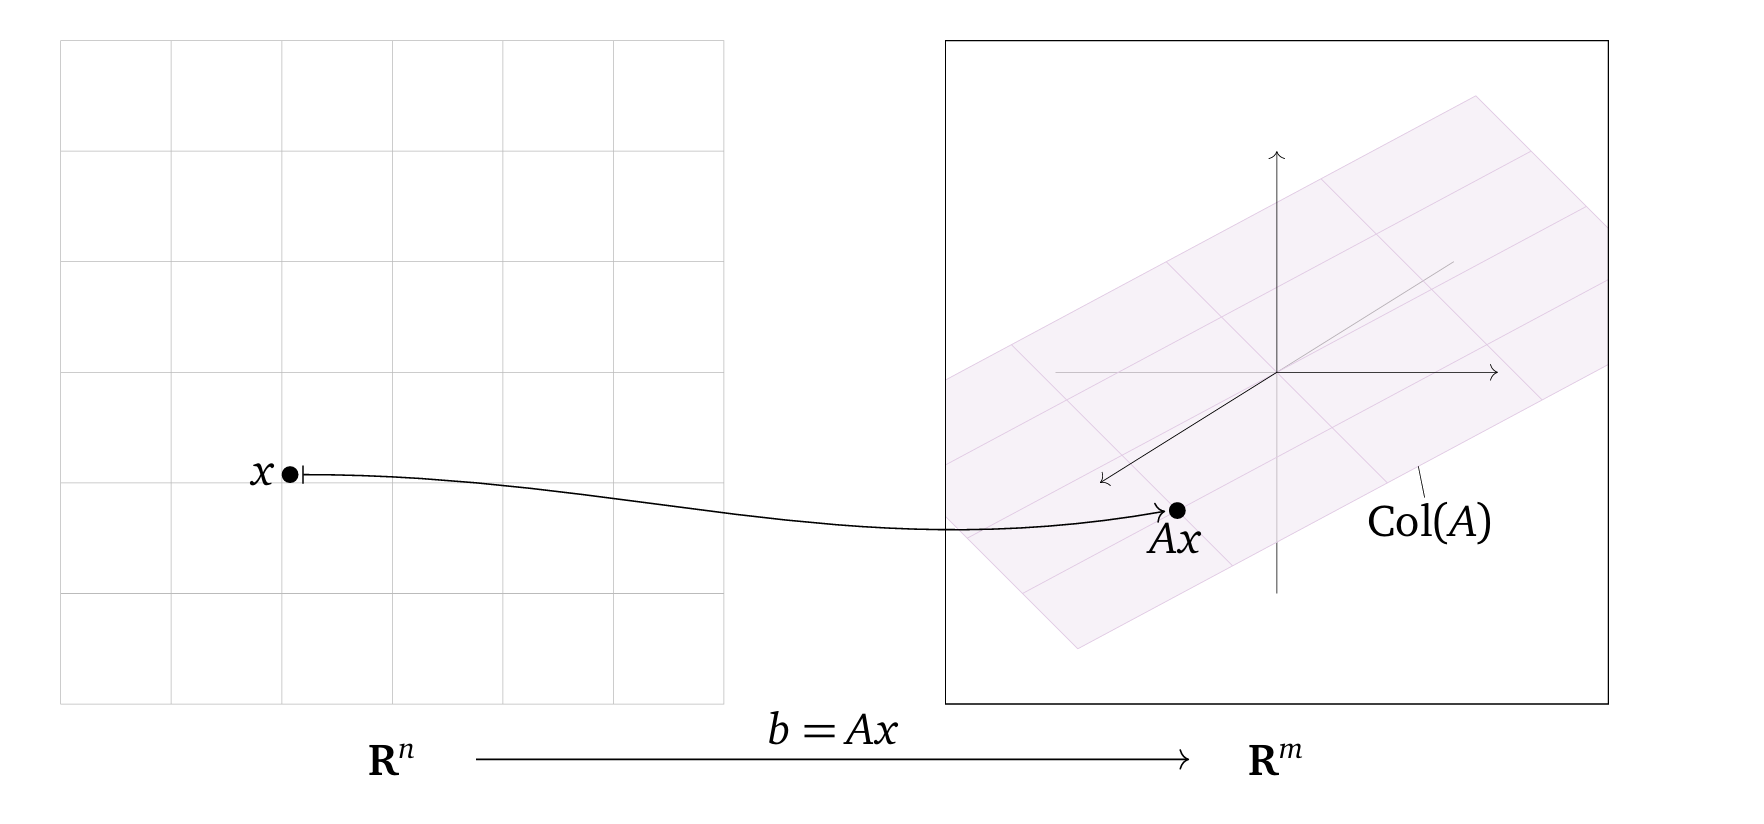
\includegraphics[width=1\linewidth]{function.png}
    \caption{Function \(b=Ax\)}
    \label{fig:enter-label}
\end{figure}

So what's the difference between normal function and matrix as function? Let see some examples.

\textbf{Example 1}. Let:

\[
    A = 
    \left( \begin{array}{cc}
    -1 & 0\\
    0 & 1
    \end{array} \right)
\]

Describe the function \(b=Ax\) geometrically.

\textbf{Solutions:} In the equation \(Ax=b\), the input vector x and the output vector b both in \(R^2\). First we multiply A by a vector to see what it does:
\[
    A
     \left( \begin{array}{c}
    x\\
    y
    \end{array} \right) 
    = 
    \left( \begin{array}{cc}
    -1 & 0\\
    0 & 1
    \end{array} \right)
    \left( \begin{array}{c}
    x\\
    y
    \end{array} \right)
    =
    \left( \begin{array}{c}
    -x\\
    y
    \end{array} \right)
\]

Multiplication with A negates the coordinate x: it \textit{ reflects on the y-axis}
\begin{figure}[H]
    \centering
    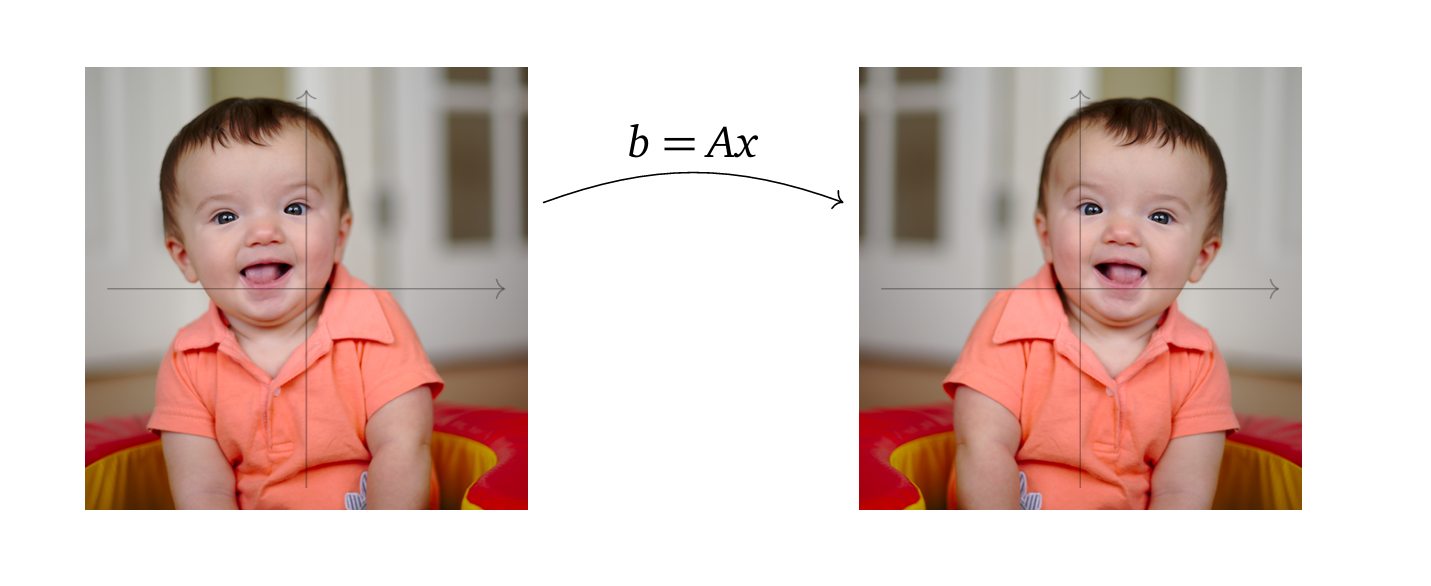
\includegraphics[width=0.75\linewidth]{reflect-Y.png}
    \label{fig:enter-label}
\end{figure}
\textbf{Example 2}. Let:
\[
    A = 
    \left( \begin{array}{cc}
    1.5 & 0\\
    0 & 1.5
    \end{array} \right)
\]

Describe the function \(b=Ax\) geometrically.

\textbf{Solutions:} In the equation \(Ax=b\), the input vector x and the output vector b both in \(R^2\). First we multiply A by a vector to see what it does:
\[
    A
     \left( \begin{array}{c}
    x\\
    y
    \end{array} \right) 
    = 
    \left( \begin{array}{cc}
    1.5 & 0\\
    0 & 1.5
    \end{array} \right)
    \left( \begin{array}{c}
    x\\
    y
    \end{array} \right)
    =
    \left( \begin{array}{c}
    1.5x\\
    1.5y
    \end{array} \right)
    =
    1.5
    \left( \begin{array}{c}
    x\\
    y
    \end{array} \right)
\]

Multiplication by A is the same as scalar multiplication by 1.5: it \textit{scales} or \textit{dilates the plane by a factor of 1.5}.
\begin{figure}[H]
    \centering
    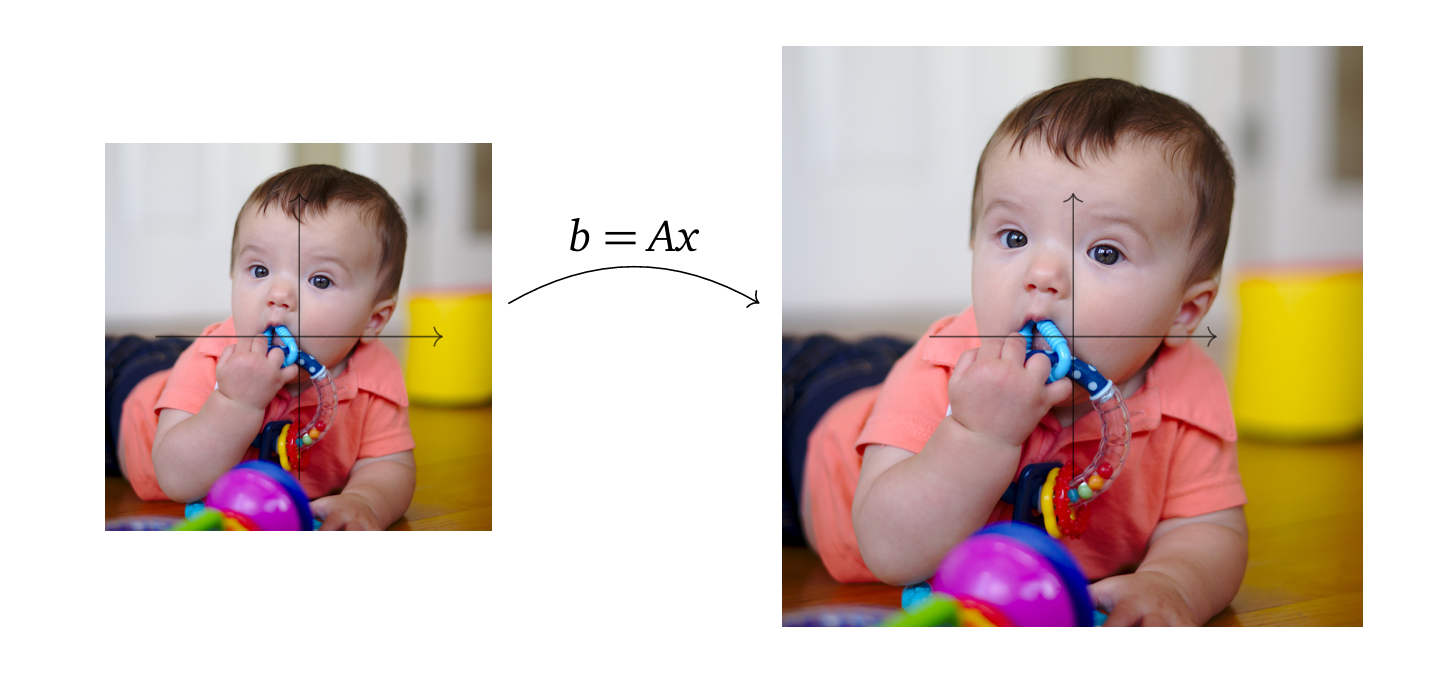
\includegraphics[width=1\linewidth]{1.5.png}
    \label{fig:enter-label}
\end{figure}

With the examples above, we have seen function matrices and how they work. In fact, function matrices are used in many research fields, and we will continue to explore them in the following sections. 

\subsubsection{Transformations}

\begin{tcolorbox}[title=Definition,colframe=blue!70!black, colback=blue!5!white]
A \textbf{\textit{transformation}} from \(\mathbb{R}^n\) to \(\mathbb{R}^m\) is a rule $T$ that assigns to each vector $x$ in \(\mathbb{R}^n\) a vector $T(x)$ in \(\mathbb{R}^m\). 
\end{tcolorbox}

\subparagraph{Example 1:}Most of the functions that you may have seen previously have a domain and a co-domain equal to
$\mathbb{R}$. For example,

\[
f: \mathbb{R} \to \mathbb{R}, \
\]
\[
\quad x \longmapsto \sin(x)
\]
Notice that we have defined $\sin$ by a rule: a function is defined by specifying what the output of the function is for any possible input.

You may be used to thinking of such functions in terms of their graphs:
\begin{center}
\begin{tikzpicture}
\begin{axis}[
    axis lines = middle,
    xlabel = {$x$},
    ylabel = {$y$},
]
% Plot sin(x)
\addplot[smooth, domain=-2*pi:2*pi, samples=100, color=blue] {sin(deg(x))};
\end{axis}
\end{tikzpicture}
\end{center}

In this case, the horizontal axis is the domain, and the vertical axis is the codomain. This is useful when the domain and codomain are $\mathbb{R}$, but it is hard to do when, for instance, the domain is $\mathbb{R}^2$ and the codomain is $\mathbb{R}^3$.
The graph of such a function is a subset of $\mathbb{R}^5$, which is difficult to visualize. For this reason, we will rarely graph a transformation.

\subparagraph{Example 2:}The definition of \textit{transformation} and its associated vocabulary may seem quite abstract, but transformations are extremely common in real life. Here is an example from the fields of robotics and computer graphics.
\begin{figure}[H]
    \centering
    \includegraphics[width=1\linewidth]{Images/roboticarm.png}
    \caption{$f:$ \(\mathbb{R}^3\) $\rightarrow$ \(\mathbb{R}^2\)\\
    \quad $f(\theta,\phi,\psi)$ $\longmapsto$ $(x,y)$
    }
    \label{fig:robotic-arm}
\end{figure}


Suppose you are building a robot arm with three joints that can move its hand around a plane, as in the following picture.

\subsubsection{Matrix Transformations}

\begin{tcolorbox}[title=Definition,colframe=blue!70!black, colback=blue!5!white]
Let $A$ be an $m \times n$ matrix. We have:
\begin{center}
T: \(\mathbb{R}^n\) \rightarrow \(\mathbb{R}^m\) \text{defined by} $T(x)=Ax$.
\end{center}
\end{tcolorbox}
If $A$ has $n$ columns, then it only makes sense to multiply $A$ by vectors with $n$ entries. This is why the domain of $T(x) = Ax$ is $\mathbb{R}^n$.  
If $A$ has $m$ rows, then $Ax$ has $m$ entries for any vector $x$ in $\mathbb{R}^n$; this is why the codomain of $T(x) = Ax$ is $\mathbb{R}^m$.

Suppose that \( A \) has columns \( \mathbf{v}_1, \mathbf{v}_2, \ldots, \mathbf{v}_n \). If we multiply \( A \) by a general vector \( \mathbf{x} \), we get
\[
A\mathbf{x} = A
\begin{pmatrix}
\mathbf{v}_1 & \mathbf{v}_2 & \cdots & \mathbf{v}_n
\end{pmatrix}
\begin{pmatrix}
x_1 \\
x_2 \\
\vdots \\
x_n
\end{pmatrix}
= x_1\mathbf{v}_1 + x_2\mathbf{v}_2 + \cdots + x_n\mathbf{v}_n.
\]
This is just a general linear combination of \( \mathbf{v}_1, \mathbf{v}_2, \ldots, \mathbf{v}_n \). The outputs of \( T(\mathbf{x}) = A\mathbf{x} \) are exactly the linear combinations of the columns of \( A \): the range of \( T \) is the column space of \( A \).

\paragraph{Properties:}Let \( A \) be an \( m \times n \) matrix, and let \( T(x) = Ax \) be the associated matrix transformation.

\begin{itemize}
    \item The domain of \( T \) is \( \mathbb{R}^n \), where \( n \) is the number of columns of \( A \).
    \item The codomain of \( T \) is \( \mathbb{R}^m \), where \( m \) is the number of rows of \( A \).
    \item The range of \( T \) is the column space of \( A \).
\end{itemize}

\subparagraph{Example 1:}Let 
\[
A = \begin{pmatrix} 1 & 0 & 0 \\ 0 & 1 & 0 \\ 0 & 0 & 0 \end{pmatrix}, \text{and let \( T(x) = Ax \).}
\]


\textbf{Domain, Codomain, and Range of \( T \):}

\begin{itemize}
    \item \textbf{Domain}: The domain of \( T \) is \( \mathbb{R}^3 \) because the input vector \( x \) has three entries.
    \item \textbf{Codomain}: The codomain of \( T \) is also \( \mathbb{R}^3 \) because the transformation maps vectors in \( \mathbb{R}^3 \) to vectors in \( \mathbb{R}^3 \).
    \item \textbf{Range}: The range of \( T \) consists of all vectors that lie on the \( xy \)-plane, because the transformation projects vectors directly onto the \( xy \)-plane. Every point on the \( xy \)-plane is an output of \( T \), with the last entry always being zero. Hence, the range of \( T \) is the \( xy \)-plane in \( \mathbb{R}^3 \).
\end{itemize}

\textbf{Geometrical Interpretation:}

The transformation \( T \) geometrically projects any vector in \( \mathbb{R}^3 \) onto the \( xy \)-plane by setting the \( z \)-coordinate to zero. This means:
\[
T \left( \begin{pmatrix} x_1 \\ x_2 \\ x_3 \end{pmatrix} \right) = \begin{pmatrix} x_1 \\ x_2 \\ 0 \end{pmatrix}.
\]

Thus, the outputs of \( T \) are always vectors of the form \( \begin{pmatrix} x_1 \\ x_2 \\ 0 \end{pmatrix} \), where \( x_1, x_2 \) are arbitrary real numbers, and the third component is always zero.

\subparagraph{Example 2:}

Let 
\[
A = \begin{pmatrix} 1 & 1 \\ 0 & 1 \\ 1 & 1 \end{pmatrix},
\]
and let \( T(x) = Ax \), so \( T: \mathbb{R}^2 \to \mathbb{R}^3 \) is a matrix transformation.

\textbf{Evaluate \( T(u) \) for \( u = \begin{pmatrix} 3 \\ 4 \end{pmatrix} \):}

We evaluate \( T(u) \) by performing matrix multiplication:
\[
T\left( \begin{pmatrix} 3 \\ 4 \end{pmatrix} \right) = A \begin{pmatrix} 3 \\ 4 \end{pmatrix} = \begin{pmatrix} 1 & 1 \\ 0 & 1 \\ 1 & 1 \end{pmatrix} \begin{pmatrix} 3 \\ 4 \end{pmatrix} = \begin{pmatrix} 7 \\ 4 \\ 7 \end{pmatrix}.
\]

\textbf{Find a vector \( v \) such that \( T(v) = b \), where \( b = \begin{pmatrix} 7 \\ 5 \\ 7 \end{pmatrix} \):}

We want to solve the equation \( Av = b \). This gives us the system of equations:
\[
\begin{pmatrix} 1 & 1 \\ 0 & 1 \\ 1 & 1 \end{pmatrix} \begin{pmatrix} x \\ y \end{pmatrix} = \begin{pmatrix} 7 \\ 5 \\ 7 \end{pmatrix}.
\]
This translates to the system:
\[
x + y = 7,
\]
\[
y = 5,
\]
\[
x + y = 7.
\]
Substitute \( y = 5 \) into the first and third equations:
\[
x + 5 = 7 \quad \Rightarrow \quad x = 2.
\]
Thus, \( v = \begin{pmatrix} 2 \\ 5 \end{pmatrix} \).

\textbf{Is there more than one solution?}

Since the system of equations has a unique solution, there is only one vector \( v \) such that \( T(v) = b \).

\textbf{Does there exist a vector \( w \) in \( \mathbb{R}^3 \) such that the solution set of \( Av = w \) has more than one vector in it?}

The solution set of \( Av = w \), if non-empty, is a translate of the solution set of \( Av = b \), which has one vector in it. Thus, the solution set of \( Av = w \) can have at most one vector.

\textbf{Find a vector \( w \) such that the matrix equation \( Av = w \) is not consistent.}

Notice that if we take
\[
w = \begin{pmatrix} 1 \\ 2 \\ 3 \end{pmatrix},
\]
then the matrix equation \( Av = w \) translates into the system of equations:
\[
x + y = 1,
\]
\[
y = 2,
\]
\[
x + y = 3,
\]
which is clearly inconsistent.

\subparagraph{Example 3:}

Define a transformation \( T: \mathbb{R}^2 \to \mathbb{R}^3 \) by the formula
\[
T\begin{pmatrix} x \\ y \end{pmatrix} = \begin{pmatrix} \ln(x) \\ \cos(y) \\ \ln(x) \end{pmatrix}.
\]

\textbf{Solution: evaluate \( T(u) \) for \( u = \begin{pmatrix} 1 \\ \pi \end{pmatrix} \):}

We evaluate \( T(u) \) using the defining formula:
\[
T\begin{pmatrix} 1 \\ \pi \end{pmatrix} = \begin{pmatrix} \ln(1) \\ \cos(\pi) \\ \ln(1) \end{pmatrix} = \begin{pmatrix} 0 \\ -1 \\ 0 \end{pmatrix}.
\]

\textbf{Let \( b = \begin{pmatrix} 7 \\ 17 \\ 7 \end{pmatrix} \). Find a vector \( v \) in \( \mathbb{R}^2 \) such that \( T(v) = b \). Is there more than one?}

We want to find \( v = \begin{pmatrix} x \\ y \end{pmatrix} \) such that:
\[
T\begin{pmatrix} x \\ y \end{pmatrix} = \begin{pmatrix} \ln(x) \\ \cos(y) \\ \ln(x) \end{pmatrix} = \begin{pmatrix} 7 \\ 17 \\ 7 \end{pmatrix}.
\]
This gives the system:
\[
\ln(x) = 7,
\]
\[
\cos(y) = 17,
\]
\[
\ln(x) = 7.
\]
Since \( \cos(y) = 17 \) is not possible (because \( \cos(y) \) must be between -1 and 1), there is no solution.

\textbf{Find a vector \( w \) in \( \mathbb{R}^3 \) which is not in the range of \( T \).}

Since \( \cos(y) \) is always between -1 and 1, any vector \( w = \begin{pmatrix} x \\ y \\ z \end{pmatrix} \) where \( y \notin [-1, 1] \) is not in the range of \( T \). For example:
\[
w = \begin{pmatrix} 0 \\ 2 \\ 0 \end{pmatrix}
\]
is not in the range of \( T \).
\subsection{One-to-one and Onto Transformations}
When studying transformations in linear algebra, two key questions we ask are whether the transformation is \textbf{\textit{one-to-one}} and whether it is \textbf{\textit{onto}}. These questions help us understand how the transformation works and how it maps elements between spaces.

To make these ideas clearer, think of a transformation as a process that takes inputs from one set (often a vector space) and produces outputs in another. A transformation is one-to-one (or injective) if each output corresponds to a unique input, meaning no two inputs map to the same output. On the other hand, a transformation is onto (or surjective) if every output has at least one corresponding input, meaning the transformation covers the entire output space.

\subsubsection{One-to-one Transformations} A \textit{one-to-one transformation} (or \textit{injection}) means that every input maps to a unique output---no two different inputs share the same output.

Imagine assigning people to seats at a concert. If it's one-to-one, each person sits in their own seat, and no two people share one.

For a matrix transformation \( T(x) = Ax \), it's one-to-one if different inputs always lead to different outputs, meaning the matrix \( A \) has linearly independent columns.

In short, a one-to-one transformation ensures that each input has its own unique output.

\begin{tcolorbox}[title=Definition (One-to-one transformations),colframe=blue!70!black, colback=blue!5!white]
A transformation:
\begin{center}
    $T$: \(\mathbb{R}^n\) $\rightarrow$ \(\mathbb{R}^m\)
\end{center}

is \textbf{\textit{one-to-one}} if, for every vector $b$ in \(\mathbb{R}^m\), the equation $T(x) = b$ has at most one solution $x$ in \(\mathbb{R}^n\). 
\end{tcolorbox}
Or in Calculus, we say:
\begin{center}
    $\forall x_1,x_2 \in X; x_1 \neq x_2 \Rightarrow{} T(x_1) \neq T(x_2)$
\end{center}

Here are some equivalent ways of saying that $T$ is \textbf{\textit{NOT}} one-to-one:
\begin{itemize}
    \item For every vector $b$ in \(\mathbb{R}^m\), the equation $T(x) = b$ has zero or one solution $x$ in \(\mathbb{R}^n\).
    \item There are two different inputs of $T$ with the same output.
    \item There exist vectors $u,v$ such that $u \neq v$, but $T(u)=T(v)$.
\end{itemize}
\begin{tcolorbox}[title=Theorem (One-to-one transformations),colframe=blue!70!black, colback=blue!5!white]
Let \( A \) be an \( m \times n \) matrix and \( T(x) = Ax \) the associated transformation. The following are equivalent:

\begin{enumerate}
    \item \( T \) is one-to-one.
    \item For every \( b \in \mathbb{R}^m \), the equation \( T(x) = b \) has at most one solution.
    \item For every \( b \in \mathbb{R}^m \), \( Ax = b \) has either a unique solution or no solution.
    \item The homogeneous system \( Ax = 0 \) has only the trivial solution.
    \item The columns of \( A \) are linearly independent.
    \item \( A \) has a pivot in every column.
    \item The range of \( T \) has dimension \( n \).
\end{enumerate}
\end{tcolorbox}
\subparagraph{Example 1: A matrix transformation that is one-to-one} Let \( A \) be the matrix

\[
A = \begin{pmatrix} 
1 & 0 \\
0 & 1 \\
0 & 0
\end{pmatrix}
\]

and define \( T: \mathbb{R}^2 \to \mathbb{R}^3 \) by \( T(x) = Ax \).

\textbf{Is \( T \) one-to-one?}

\textbf{Solution:}  
The reduced row echelon form of \( A \) is

\[
A = \begin{pmatrix} 
1 & 0 \\
0 & 1 \\
0 & 0
\end{pmatrix}
\]

Hence, \( A \) has a pivot in every column, so \( T \) is one-to-one.

\subparagraph{Example 2: A matrix transformation that is not one-to-one} Let \( A \) be the matrix

\[
A = \begin{pmatrix} 
1 & 1 & 0 \\
0 & 1 & 1
\end{pmatrix}
\]

and define \( T: \mathbb{R}^3 \to \mathbb{R}^2 \) by \( T(x) = Ax \).

\textbf{Is \( T \) one-to-one?} 

\textbf{Solution:}  
The reduced row echelon form of \( A \) is

\[
A = \begin{pmatrix} 
1 & 0 & -1 \\
0 & 1 & 1
\end{pmatrix}
\]

There is not a pivot in every column, so \( T \) is not one-to-one. Therefore, we know from the fact that \( Ax = 0 \) has nontrivial solutions. If \( v \) is a nontrivial (i.e., nonzero) solution of \( Av = 0 \), then \( T(v) = Av = 0 = A0 = T(0) \), so 0 and \( v \) are different vectors with the same output.

In order to find a nontrivial solution, we find the parametric form of the solutions of \( Ax = 0 \) using the reduced matrix above:

\[
\begin{aligned}
x - z &= 0 \\
y + z &= 0
\end{aligned}
\]

\[
\Rightarrow
\begin{pmatrix}
x \\
y \\
z
\end{pmatrix}
= 
\begin{pmatrix}
z \\
-z \\
z
\end{pmatrix}
\]

The free variable is \( z \). Taking \( z = 1 \) gives the nontrivial solution:

\[
\begin{pmatrix}
1 \\
-1 \\
1
\end{pmatrix}
\]

Thus, \( T\left( \begin{pmatrix} 1 \\ -1 \\ 1 \end{pmatrix} \right) = 
\begin{pmatrix}
    1 & 1 & 0\\
    0 & 1 & 1
\end{pmatrix}\begin{pmatrix}
    1\\-1\\1
\end{pmatrix}
= 0 = T\begin{pmatrix}
    0\\0\\0
\end{pmatrix} \).

\subsubsection{Onto Transformation}
An \textit{onto transformation} (or \textit{surjection}) means that every point in the target space has at least one corresponding point in the domain. In simpler terms, every possible output is covered by some input.

Imagine you're assigning people to seats at a concert. If it's "onto," every seat gets filled by at least one person, even if some people take multiple seats. No seat is left empty.

For a matrix transformation \( T(x) = Ax \), it's onto if every point in the target space can be reached from the domain. This usually means that the matrix \( A \) has enough coverage to map to the entire target space.

In short, an onto transformation ensures every possible output has a matching input.

\begin{tcolorbox}[title=Definition (Onto Transformation),colframe=blue!70!black, colback=blue!5!white]
A transformation \( T: \mathbb{R}^n \to \mathbb{R}^m \) is onto if for every vector \( b \) in the target space \( \mathbb{R}^m \), there exists at least one vector \( x \) in the domain \( \mathbb{R}^n \) such that 

\[T(x) = b.\]
\end{tcolorbox}
Or in calculus we say:
\[
    \forall y \in Y ,\exists x \in X : f(x) = y.\\
\]
Here are some equivalent ways of saying that $T$ is onto:
\begin{itemize}
    \item The range of $T$ is equal to the codomain of $T$.
    \item Every vector in the codomain is the output of some input vector.
\end{itemize}

Here are some equivalent ways of saying that $T$ is not onto:
\begin{itemize}
    \item The range of $T$ is smaller than the codomain of $T$.
    \item There exists a vector $b$ in \(\mathbb{R}^m\) such that the equation $T(x) = b$ does not have a solution.
    \item There is a vector in the codomain that is not the output of any input vector.
.
\end{itemize}
Suppose \( T(x) = Ax \) is a matrix transformation that is not onto. This means the range of \( T \), or \( \text{Col}(A) \), is a subspace of \( \mathbb{R}^m \) with dimension less than \( m \). The range is much smaller than the codomain, like a line in 2D or 3D space, or a plane in 3D. 

To find a vector not in the range of \( T \), you can pick any random nonzero vector \( b \in \mathbb{R}^m \). It's very unlikely that \( b \) will be in the range of \( T \). To check if \( b \) is in the range, solve the matrix equation \( Ax = b \) to see if it's consistent.


\begin{tcolorbox}[title=Attention!,colframe=blue!70!black, colback=blue!5!white]
Tall matrices do not have onto transformations. If \( T : \mathbb{R}^n \to \mathbb{R}^m \) is an onto matrix transformation, what can we say about the relative sizes of \( n \) and \( m \)?

The matrix associated with \( T \) has \( n \) columns and \( m \) rows. Each row and each column can only contain one pivot, so in order for \( A \) to have a pivot in every row, it must have at least as many columns as rows: \( m \leq n \).

This says that, for instance, \( \mathbb{R}^2 \) is “too small” to admit an onto linear transformation to \( \mathbb{R}^3 \).

Note that there exist wide matrices that are not onto.
\end{tcolorbox}
For example, 
\[
G = \begin{pmatrix} 
10 & 2 & 3 \\
1 & -1 & 4
\end{pmatrix}
\]
does not have a pivot in every row.

\subsubsection{Comparison between onto \& one-to-one}
We’ve provided a table here to help you compare two important types of transformations: one-to-one (injective) and onto (surjective). These concepts are key in understanding functions, and knowing the difference between them is essential. The table below makes it easier to see how these two types of transformations work.
\[
\begin{array}{|c|c|}
\hline
\textbf{T is one-to-one} & \textbf{T is onto} \\
\hline
T(x) = b \text{ has at most one solution for every } b. & T(x) = b \text{ has at least one solution for every } b. \\
\hline
\text{The columns of } A \text{ are linearly independent.} & \text{The columns of } A \text{ span } \mathbb{R}^m. \\
\hline
A \text{ has a pivot in every column.} & A \text{ has a pivot in every row.} \\
\hline
\text{The range of } T \text{ has dimension } n. & \text{The range of } T \text{ has dimension } m. \\
\hline
\end{array}
\]
By taking a closer look, you'll be able to clearly tell the difference: a one-to-one function ensures that every element in the domain is paired with a unique element in the codomain, while an onto function guarantees that every element in the codomain has at least one corresponding element in the domain.
\subsection{Linear Transformation}
In this section, we change our approach. Instead of thinking of matrices as functions, we focus on a transformation we want to understand. If we can show that the transformation is a matrix transformation, we can apply linear algebra to study it. This brings up two key questions:
\begin{enumerate}
    \item How can we determine if a transformation is a matrix transformation?
    \item If it is, how can we find the matrix that represents it?
\end{enumerate}

For example, consider the matrix transformation:

\[
T: \mathbb{R}^2 \to \mathbb{R}^2, \quad T(x) = \begin{pmatrix} 0 & -1 \\ 1 & 0 \end{pmatrix} x
\]

This represents a counterclockwise rotation of the plane by \(90^\circ\). However, we could describe \(T\) in a more abstract way:

\[
T: \mathbb{R}^2 \to \mathbb{R}^2, \quad T(x) = \text{the counterclockwise rotation of } x \text{ by } 90^\circ.
\]

In this form, it's not immediately clear that \(T\) is a matrix transformation, or what matrix it corresponds to.

\begin{tcolorbox}[title=Definition,colframe=blue!70!black, colback=blue!5!white]
A \textbf{\textit{linear transformation}} is a transformation $T:$ \(\mathbb{R}^n\) $\rightarrow$ \(\mathbb{R}^m\) satisfying:
\begin{itemize}
    \item $T(u+v) = T(u) + T(v)$. \quad ("additivity")
    \item $T(cu) = cT(u)$. \quad ("homogeneity")
\end{itemize}
for all vectors $u,v$ in \(\mathbb{R}^n\) and all scalars $c$.
\end{tcolorbox}

Let $T:\mathbb{R}^n \rightarrow \mathbb{R}^m$ be a matrix transformation $T(x)=Ax$ for an $m \times n$ matrix $A$. By this proposition in Section \ref{matrix-vector-product}, we have:
\[
T(u+v)=A(u+v)=Au+Av=T(u)+T(v)
T(cu)=A(cu)=cAu=cT(u)
\]

Since both properties hold, we can conclude that matrix transformations are indeed linear transformations.

\subparagraph{Key Insight}

In the next section, we’ll see that every linear transformation is, in fact, a matrix transformation. This means that for any linear transformation, there is always a matrix that represents it. We might not know the matrix right away, but it’s always possible to find one.

\subparagraph{Important Facts about Linear Transformations}

Let $T: \mathbb{R}^n \to \mathbb{R}^m$ be a linear transformation. Then the following facts hold:

\begin{enumerate}
    \item \textbf{Zero Vector Mapping}:
    \[
    T(0) = 0.
    \]
    This means that a linear transformation always maps the zero vector to the zero vector. This is a fundamental property of linear transformations.

    \item \textbf{Superposition Principle}: For any vectors $v_1, v_2, \dots, v_k$ in $\mathbb{R}^n$ and scalars $c_1, c_2, \dots, c_k$, we have:
    \[
    T(c_1v_1 + c_2v_2 + \dots + c_kv_k) = c_1T(v_1) + c_2T(v_2) + \dots + c_kT(v_k).
    \]
    This is known as the \textit{superposition principle} and reflects how linear transformations distribute over vector addition and scalar multiplication. For example, if we have vectors $u$ and $v$ and scalars $c$ and $d$, we can apply the transformation $T$ as follows:
    \[
    T(cu + dv) = cT(u) + dT(v).
    \]
    This ensures that linear transformations behave in a predictable and additive manner.
\end{enumerate}

\subsubsection{The Standard Coordinate Vectors}
\paragraph{Standard coordinate vectors}
he standard coordinate vectors in $\mathbb{R}^n$ are the $n$ vectors

\[
\mathbf{e}_1 = \begin{pmatrix} 1 \\ 0 \\ \vdots \\ 0 \end{pmatrix}, \quad 
\mathbf{e}_2 = \begin{pmatrix} 0 \\ 1 \\ \vdots \\ 0 \end{pmatrix}, \quad \dots, \quad
\mathbf{e}_{n-1} = \begin{pmatrix} 0 \\ \vdots \\ 1 \\ 0 \end{pmatrix}, \quad
\mathbf{e}_n = \begin{pmatrix} 0 \\ \vdots \\ 0 \\ 1 \end{pmatrix}.
\]

The $i$th entry of $\mathbf{e}_i$ is equal to 1, and the other entries are zero.

From now on, for the rest of the book, we will use the symbols $\mathbf{e}_1, \mathbf{e}_2, \dots$ to denote the standard coordinate vectors.

There is an inherent ambiguity in the notation of the standard coordinate vectors. Specifically, when we write $\mathbf{e}_1$, we must rely on the context to understand how many entries are in the vector. This means that the vector

\[
\mathbf{e}_1 = \begin{pmatrix} 1 \\ 0 \end{pmatrix}
\]

could be interpreted as a two-dimensional vector in $\mathbb{R}^2$, but it could also refer to

\[
\mathbf{e}_1 = \begin{pmatrix} 1 \\ 0 \\ 0 \end{pmatrix}
\]

in the case of $\mathbb{R}^3$, depending on the space we are working in. Both vectors are denoted by the same symbol, $\mathbf{e}_1$, but the number of entries—i.e., the dimension of the vector—differs depending on whether we are considering vectors in $\mathbb{R}^2$ or $\mathbb{R}^3$. This can lead to confusion unless the dimension of the space is explicitly stated or can be inferred from the context.

For example, in two-dimensional space, the standard coordinate vectors are:

\[
\mathbf{e}_1 = \begin{pmatrix} 1 \\ 0 \end{pmatrix}, \quad \mathbf{e}_2 = \begin{pmatrix} 0 \\ 1 \end{pmatrix}.
\]

These vectors have two entries each, corresponding to the $x$ and $y$ axes in the 2D plane. On the other hand, in three-dimensional space, the standard coordinate vectors are:

\[
\mathbf{e}_1 = \begin{pmatrix} 1 \\ 0 \\ 0 \end{pmatrix}, \quad \mathbf{e}_2 = \begin{pmatrix} 0 \\ 1 \\ 0 \end{pmatrix}, \quad \mathbf{e}_3 = \begin{pmatrix} 0 \\ 0 \\ 1 \end{pmatrix}.
\]

Here, each vector has three entries, corresponding to the $x$, $y$, and $z$ axes in 3D space. Notice that the notation $\mathbf{e}_1$ in both of these cases refers to different vectors—one with two entries and one with three. Therefore, it’s essential to keep in mind the dimensionality of the space when using or interpreting standard coordinate vectors. This will help avoid any confusion about the number of entries the vectors have.

The standard coordinate vectors in \(\mathbb{R}^2\) and \(\mathbb{R}^3\) are pictured below.
\begin{figure}[H]
    \centering
    \includegraphics[width=1\linewidth]{Images/thestandard.png}
    \caption{\centering These are the vectors of length 1 that point in the positive directions of each of the axes.}
    \label{fig:coordinate-vectors}
\end{figure}
\paragraph{Multiplying a matrix by the standard coordinate vectors} If $A$ is an $m \times n$ matrix with columns $v_1, v_2,\dots v_m$, then $Ae_i=v_i$ for each $i = 1,2,\dots,n$:
\[
\begin{pmatrix}
    | & | & \quad & |\\
    v_1 & v_2 & \dots & v_n\\
    | & | & \quad & |
\end{pmatrix} e_i = v_i
\]


\begin{tcolorbox}[title=Definition,colframe=blue!70!black, colback=blue!5!white]
The $n \times n$ \textit{\textbf{identity matrix}} is the matrix $I_n$ whose columns are the $n$ standard coordinate vectors in \(\mathbb{R}^n\)
\[
I_n = \begin{pmatrix}
    1 & 0 & \dots & 0 & 0 \\
    0 & 1 & \dots & 0 & 0 \\
    \vdots & \vdots & \ddots & \vdots & \vdots \\
    0 & 0 & \dots & 1 & 0 \\
    0 & 0 & \dots & 0 & 1
\end{pmatrix}.
\]
\end{tcolorbox}

\subsubsection{The Matrix of a Linear Transformation}

\begin{tcolorbox}[title=Theorem (The matrix of a linear transformation),colframe=blue!70!black, colback=blue!5!white]
Let $T:$ \(\mathbb{R}^n\) $\rightarrow$ \(\mathbb{R}^m\) be a linear transformation. Let $A$ be the $m \times n$ matrix.
\[
A = \begin{pmatrix}
    | & | & \quad & | \\
    T(e_1) & T(e_2) & \dots & T(e_n) \\
    | & | & \quad & |
\end{pmatrix}.
\]
$\Rightarrow$ Then $T$ is the \textit{\textbf{matrix transformation}} associated with $A$: that is, $T(x)=Ax$.
\end{tcolorbox}

\subparagraph{Proof:}We suppose for simplicity that \( T \) is a transformation from \( \mathbb{R}^3 \) to \( \mathbb{R}^2 \). Let \( A \) be the matrix given in the statement of the theorem. Then

\[
T\begin{pmatrix} x \\ y \\ z \end{pmatrix}
= T\begin{pmatrix} x \\ 0 \\ 0 \end{pmatrix} + T\begin{pmatrix} 0 \\ y \\ 0 \end{pmatrix} + T\begin{pmatrix} 0 \\ 0 \\ z \end{pmatrix}
\]
\[
= T\left( x e_1 + y e_2 + z e_3 \right)
= x T(e_1) + y T(e_2) + z T(e_3)
= \begin{pmatrix} T(e_1) & T(e_2) & T(e_3) \end{pmatrix} \begin{pmatrix} x \\ y \\ z \end{pmatrix}
= A \begin{pmatrix} x \\ y \\ z \end{pmatrix}.
\] 
The matrix \( A \) described in the above theorem is known as the \textit{standard matrix} for the linear transformation \( T \). Essentially, this matrix \( A \) represents the way \( T \) acts on vectors in \( \mathbb{R}^n \). The columns of \( A \) are the images of the standard coordinate vectors under the transformation \( T \). In other words, each column of the matrix corresponds to the vector that results from applying the transformation \( T \) to one of the standard basis vectors in \( \mathbb{R}^n \).

To summarize a key part of the theorem, we observe the following fundamental idea:

\[
\textbf{\text{Matrix transformations and linear transformations are, in fact, the same thing.}}
\]

This idea forms the core of the connection between linear transformations and matrices. We can think of a linear transformation as a specific type of matrix transformation, and every matrix represents a linear transformation. This relationship is summarized in a useful correspondence, which can be outlined in the following way:

\[
T: \mathbb{R}^n \to \mathbb{R}^m \quad \text{(Linear transformation)} \quad \longrightarrow \quad \text{an} \, m \times n \, \text{matrix}
\]

Here, the linear transformation \( T \) takes a vector from \( \mathbb{R}^n \) and maps it to \( \mathbb{R}^m \), and this transformation can be fully captured by an \( m \times n \) matrix.

Now, let’s consider the matrix \( A \). This matrix is formed by taking the images of the standard basis vectors of \( \mathbb{R}^n \) under the transformation \( T \). Specifically, the columns of \( A \) are the vectors \( T(e_1), T(e_2), \dots, T(e_n) \), where \( e_1, e_2, \dots, e_n \) are the standard basis vectors in \( \mathbb{R}^n \). Thus, the matrix \( A \) is given by:

\[
A = \begin{pmatrix} T(e_1) & T(e_2) & \cdots & T(e_n) \end{pmatrix}
\]

Finally, we can express the action of the linear transformation \( T \) in terms of matrix multiplication. Given a vector \( x \in \mathbb{R}^n \), the transformation \( T \) acts on \( x \) by multiplying it with the matrix \( A \), as follows:

\[
T: \mathbb{R}^n \to \mathbb{R}^m \quad T(x) = Ax \longleftarrow \text{This is the matrix corresponding to linear transformation } A.
\]
 Every linear transformation can be represented by a matrix, and every matrix transformation is a linear transformation. The matrix captures all the information about the action of the transformation on the vector space.

\subparagraph{Question:}
Verify that the identity transformation \( \text{Id}_{\mathbb{R}^n}: \mathbb{R}^n \to \mathbb{R}^n \) is linear, and compute its standard matrix.
\subparagraph{Solution:} To verify that the identity transformation \( \text{Id}_{\mathbb{R}^n} : \mathbb{R}^n \to \mathbb{R}^n \) is linear, we need to check the two properties of linearity:

1. Additivity: For any two vectors \( \mathbf{u}, \mathbf{v} \in \mathbb{R}^n \), we have:
   \[
   \text{Id}_{\mathbb{R}^n}(\mathbf{u} + \mathbf{v}) = \mathbf{u} + \mathbf{v} = \text{Id}_{\mathbb{R}^n}(\mathbf{u}) + \text{Id}_{\mathbb{R}^n}(\mathbf{v}).
   \]
   So, additivity holds.

2. Homogeneity: For any scalar \( c \) and vector \( \mathbf{u} \in \mathbb{R}^n \), we get:
   \[
   \text{Id}_{\mathbb{R}^n}(c \mathbf{u}) = c \mathbf{u} = c \, \text{Id}_{\mathbb{R}^n}(\mathbf{u}).
   \]
   Therefore, homogeneity also holds.

Since both properties are satisfied, \( \text{Id}_{\mathbb{R}^n} \) is a linear transformation.


The standard matrix of a linear transformation is determined by how it acts on the standard basis vectors. The identity transformation maps each basis vector \( e_1, e_2, \dots, e_n \) to itself:
\[
\text{Id}_{\mathbb{R}^n}(e_1) = e_1, \quad \text{Id}_{\mathbb{R}^n}(e_2) = e_2, \quad \dots, \quad \text{Id}_{\mathbb{R}^n}(e_n) = e_n.
\]
Thus, the standard matrix of \( \text{Id}_{\mathbb{R}^n} \) is the identity matrix:
\[
\Rightarrow A = I_n.
\]
\subsection{Matrix Multiplication}In this section, we explore compositions of transformations. Composition allows us to chain multiple transformations together, where the result of one transformation becomes the input for the next. Interestingly, the composition of matrix transformations is equivalent to multiplying the corresponding matrices.

We will also discuss how transformations and matrices can be added together and how they interact with scalar multiplication.
\subsubsection{Composition of linear transformations}Composition in linear algebra follows the same idea as in calculus. The definition is as follows:

\begin{tcolorbox}[title=Definition,colframe=blue!70!black, colback=blue!5!white]
Let \( T : \mathbb{R}^n \to \mathbb{R}^m \) and \( U : \mathbb{R}^p \to \mathbb{R}^n \) be transformations. Their composition is the transformation \( T \circ U : \mathbb{R}^p \to \mathbb{R}^m \), defined by:
\[
(T \circ U)(x) = T(U(x)).
\]
\end{tcolorbox}

Composing two transformations means chaining them together. The composition \( T \circ U \) is the transformation that first applies \( U \), and then applies \( T \) (note the order of operations). More precisely, to evaluate \( T \circ U \) on an input vector \( \mathbf{x} \), you first apply \( U(\mathbf{x}) \), then take this output vector of \( U \) and use it as the input for \( T \):
\[
(T \circ U)(\mathbf{x}) = T(U(\mathbf{x})).
\]
This composition is valid only when the outputs of \( U \) are valid inputs for \( T \), meaning the range of \( U \) must be contained within the domain of \( T \).

\begin{figure}[H]
    \centering
    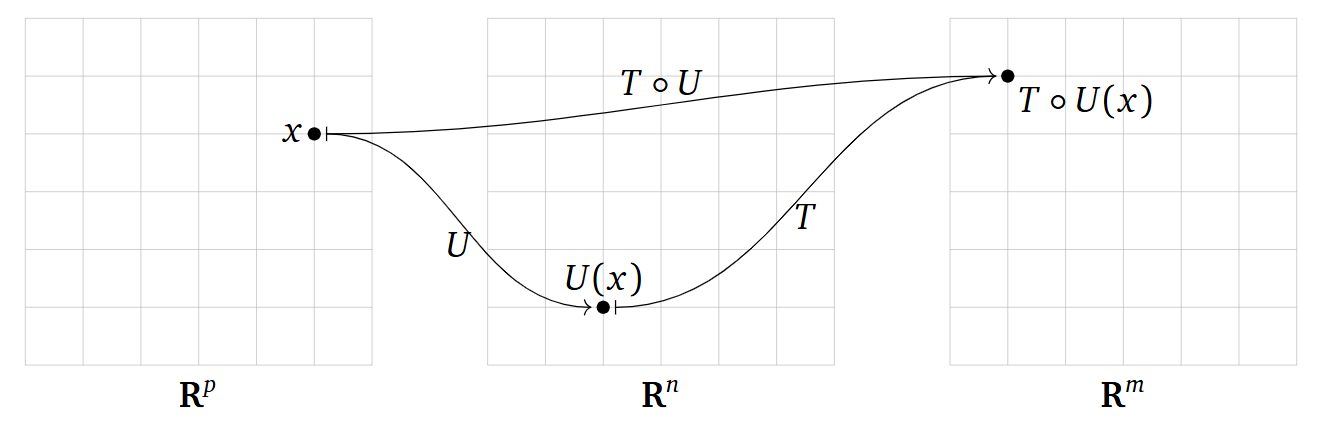
\includegraphics[width=1\linewidth]{CompositionofLT.png}
    \caption{Composition \(T \circ U\)}
    \label{fig:colt}
\end{figure}
\begin{figure}[H]
    \centering
    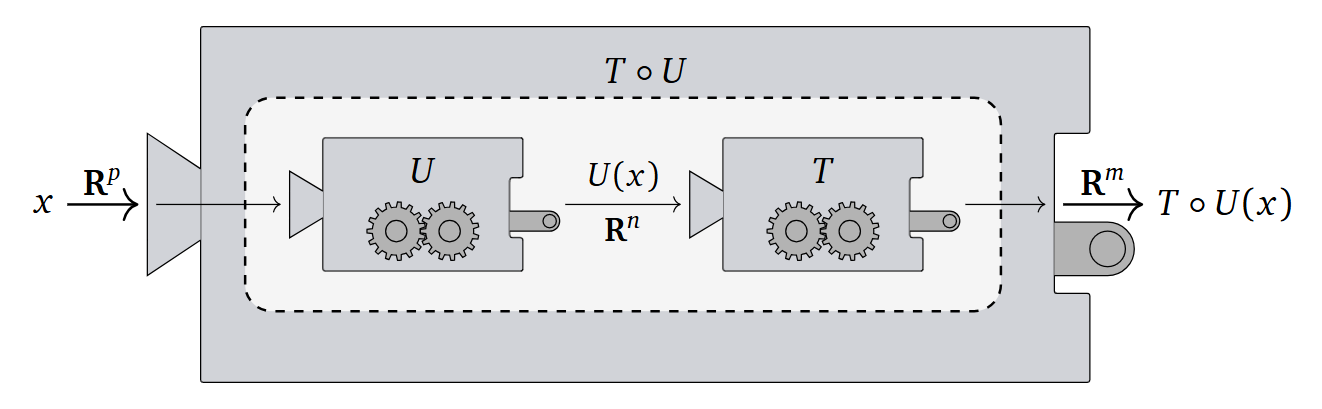
\includegraphics[width=1\linewidth]{coltasmachine.png}
    \caption{Composition \(T \circ U\)}
    \label{fig:colt-as-machine}
\end{figure}

\subparagraph{Domain and codomain of a composition}
\begin{itemize}
    \item In order for \(T \circ U\) to be defined, the codomain of $U$ must equal to the domain of $T$.
    \item The domain of \(T \circ U\) is the domain of $U$.
    \item The codomain of  \(T \circ U\) is the codomain of $T$.
\end{itemize}

\subparagraph{Example 1:}Define $f:\mathbb{R} \rightarrow \mathbb{R}$ by $f(x)=x^2$ and $g:\mathbb{R} \rightarrow \mathbb{R}$ by $g(x)=x^3$. The composition $f \circ g:\mathbb{R} \rightarrow \mathbb{R}$ is the transformation defined by the rule:
\[
(f \circ g)(x) = f(g(x)) = f(x^3) = (x^3)^2 = x^6.
\]

\subparagraph{Example 2:}Define $T:\mathbb{R}^3 \rightarrow \mathbb{R}^2$ and $U:\mathbb{R}^2 \rightarrow \mathbb{R}^3$ by 
\[
T(x) = \begin{pmatrix}
    1 & 1 & 0\\
    0 & 1 & 0
\end{pmatrix}x \quad \text{and} \quad U(x) = \begin{pmatrix}
    1 & 0 \\
    0 & 1 \\ 
    1 & 0
\end{pmatrix}x. 
\]
Their composition is a transformation $T \circ U: \mathbb{R}^2 \rightarrow \mathbb{R}^2$
$\Rightarrow$ The matrix transformation associated to the matrix $\begin{pmatrix}
    1 & 1\\
    1 & 1
\end{pmatrix}$.
\subsubsection{Matrix multiplication}\textbf{\textit{Matrix multiplication }}corresponds precisely to the \textbf{composition} of the corresponding linear transformations.
\paragraph{Terminology}Let \( A \) be an \( m \times n \) matrix. We will generally use \( a_{ij} \) to denote the entry in the \( i \)-th row and the \( j \)-th column of the matrix. This is referred to as the \textit{entry} in the \( i, j \) position of the matrix.
\begin{figure}[H]
    \centering
    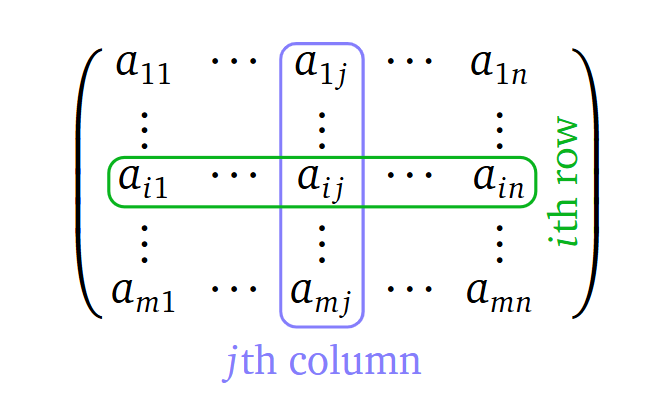
\includegraphics[width=1\linewidth]{matrixMultiplication.png}
    \label{fig:matrix-multiplication-notation}
\end{figure}
Here, \( a_{11} \) refers to the element in the first row and first column, \( a_{12} \) refers to the element in the first row and second column, and so on.\\
\begin{tcolorbox}[title=Definition (Matrix multiplication),colframe=blue!70!black, colback=blue!5!white]
Consider two matrices: \( A \), which is an \( m \times n \) matrix, and \( B \), which is an \( n \times p \) matrix. Notice that the number of columns in \( A \) must match the number of rows in \( B \) for the multiplication to be defined. The matrix product \( AB \) will result in a new matrix, which we’ll call \( C \), and \( C \) will have dimensions \( m \times p \) (i.e., the number of rows from \( A \) and the number of columns from \( B \)).

To understand this, think of the matrix \( B \) as being made up of column vectors, like this:

\[
B = \begin{pmatrix} 
| & | & | \\
v_1 & v_2 & \cdots & v_p \\
| & | & |
\end{pmatrix}
\]
\end{tcolorbox}
Here, each \( v_j \) represents the \( j \)-th column of matrix \( B \). Now, the product \( AB \) is calculated by multiplying matrix \( A \) with each of the column vectors \( v_1, v_2, \ldots, v_p \), which results in a new matrix:

\[
AB = \begin{pmatrix}
Av_1 & Av_2 & \cdots & Av_p
\end{pmatrix}
\]

In simpler terms, matrix multiplication is computed column-by-column. Each column of the resulting matrix \( AB \) is obtained by multiplying \( A \) with the corresponding column from matrix \( B \).

\paragraph{Matrix Dimensions and Multiplication Rules}

One important thing to keep in mind is the dimensional compatibility required for matrix multiplication. To perform the multiplication \( AB \), the number of columns of matrix \( A \) must equal the number of rows of matrix \( B \). Specifically:

- If \( A \) is an \( m \times n \) matrix and \( B \) is an \( n \times p \) matrix, the resulting matrix \( AB \) will have dimensions \( m \times p \).
- If matrix \( B \) has only one column, then the resulting matrix \( AB \) will also have one column. This is similar to a matrix-vector multiplication where matrix \( A \) acts on a vector (i.e., a column matrix).

Furthermore, if \( A \) is a square matrix (i.e., the number of rows equals the number of columns), then it’s possible to multiply it by itself, and we define its powers as:

\[
A^2 = A \cdot A, \quad A^3 = A \cdot A \cdot A, \quad \text{and so on.}
\]

\paragraph{Row-Column Rule for Matrix Multiplication}

To make matrix multiplication more concrete, let’s look at the row-column rule, which describes how to compute each entry of the resulting matrix.

Recall that the product of a row vector and a column vector is simply a scalar (a number). For instance, the product of the row vector \( \begin{pmatrix} a_1 & a_2 & \cdots & a_n \end{pmatrix} \) and the column vector \( \begin{pmatrix} x_1 \\ x_2 \\ \vdots \\ x_n \end{pmatrix} \) results in the scalar:

\[
a_1x_1 + a_2x_2 + \cdots + a_nx_n
\]

In matrix multiplication, the rule is similar: to find the entry \( c_{ij} \) of the product matrix \( C \), we compute the dot product of the \( i \)-th row of \( A \) and the \( j \)-th column of \( B \). This is expressed as:

\[
c_{ij} = a_{i1}b_{1j} + a_{i2}b_{2j} + \cdots + a_{in}b_{nj}
\]

This procedure is known as the \textit{row-column rule}, and it gives us an easy way to compute matrix products one entry at a time.

\[
C = AB = \begin{pmatrix} 
c_{11} & c_{12} & \cdots & c_{1p} \\
c_{21} & c_{22} & \cdots & c_{2p} \\
\vdots & \vdots & \ddots & \vdots \\
c_{m1} & c_{m2} & \cdots & c_{mp}
\end{pmatrix}
\]

For example, let’s say you want to compute the first entry \( c_{11} \) of the resulting matrix \( C \). You would multiply the first row of \( A \) by the first column of \( B \) and sum the products:

\[
c_{11} = a_{11}b_{11} + a_{12}b_{21} + \cdots + a_{1n}b_{n1}
\]

This process is repeated for each entry in the matrix.
\subparagraph{Proof:} 
\begin{equation}
A x = 
\begin{pmatrix}
r_1 \\
r_2 \\
\vdots \\
r_m
\end{pmatrix}
x = 
\begin{pmatrix}
r_1 x \\
r_2 x \\
\vdots \\
r_m x
\end{pmatrix}.
\end{equation}

The matrix multiplication is:

\[
A 
\begin{pmatrix}
c_1 \\
c_2 \\
\vdots \\
c_p
\end{pmatrix}
= 
\begin{pmatrix}
A c_1 \\
A c_2 \\
\vdots \\
A c_p
\end{pmatrix}.
\]

It follows that:

\[
\begin{pmatrix}
r_1 \\
r_2 \\
\vdots \\
r_m
\end{pmatrix}
\begin{pmatrix}
c_1 & c_2 & \cdots & c_p
\end{pmatrix}
=
\begin{pmatrix}
r_1 c_1 & r_1 c_2 & \cdots & r_1 c_p \\
r_2 c_1 & r_2 c_2 & \cdots & r_2 c_p \\
\vdots & \vdots & \ddots & \vdots \\
r_m c_1 & r_m c_2 & \cdots & r_m c_p
\end{pmatrix}.
\]
\paragraph{Properties and Caveats of Matrix Multiplication}

Matrix multiplication behaves in many ways as one would expect from regular multiplication, but there are some important caveats to keep in mind:

\begin{itemize}
    \item Non-commutativity: In general, matrix multiplication is \textit{not} commutative. This means that \( AB \neq BA \) in most cases, even when both products are defined. For instance, multiplying matrix \( A \) by matrix \( B \) may not yield the same result as multiplying \( B \) by \( A \).
    \item Cancellation law does not hold: The cancellation law, which states that if \( AB = AC \) then \( B = C \), does not always hold. This is an important property to be aware of when working with matrix equations.
    \item Zero product: It is possible for \( AB = 0 \) even if neither \( A \) nor \( B \) is the zero matrix. This can happen due to the structure of the matrices involved.
\end{itemize}

Although matrix multiplication is not commutative in general, there are some special cases where \( AB = BA \). For example, if \( A \) is the zero matrix or if \( A = B \), the multiplication will be commutative.

\paragraph{Matrix Multiplication as Composition of Transformations}

Now, let’s relate matrix multiplication to linear transformations. Let \( T: \mathbb{R}^n \to \mathbb{R}^m \) and \( U: \mathbb{R}^p \to \mathbb{R}^n \) be linear transformations, and let \( A \) and \( B \) represent their corresponding standard matrices, respectively. Recall that the composition of these transformations, \( T \circ U \), applies \( U \) to a vector \( x \) and then applies \( T \) to the result:

\[
(T \circ U)(x) = T(U(x))
\]

On the matrix side, the standard matrix for the composition \( T \circ U \) is the matrix product \( AB \), so:

\[
(T \circ U)(x) = (AB)x
\]

By associativity of matrix multiplication, we can rewrite this as:

\[
(AB)x = A(Bx)
\]

This shows that to compute the result of the composition of two transformations, we first apply \( B \) to \( x \), and then apply \( A \) to the result.

Thus, matrix multiplication directly mirrors the process of composing linear transformations. It is important to note that matrices and transformations are written in opposite order: the matrix for \( T \circ U \) is \( AB \), but the transformations are applied in the order \( U \) first, then \( T \).

\subsubsection{Composition and Matrix Multiplication}The main idea of this subsection is to demonstrate that matrix multiplication is directly related to the composition of linear transformations. In simpler terms, the standard matrix for \( T \circ U \) (the composition of transformations \( T \) and \( U \)) is simply the product of the standard matrices for \( T \) and \( U \). At first, it may seem hard to believe that the seemingly complex formula for matrix multiplication actually represents something as intuitive as "chaining two transformations together." But once we understand this connection, it becomes a powerful and insightful concept!

\begin{tcolorbox}[title=Theorem,colframe=blue!70!black, colback=blue!5!white]
Let \( T: \mathbb{R}^n \to \mathbb{R}^m \) and \( U: \mathbb{R}^p \to \mathbb{R}^n \) be linear transformations, and let \( A \) and \( B \) be their standard matrices, respectively, so \( A \) is an \( m \times n \) matrix and \( B \) is an \( n \times p \) matrix. Then \( T \circ U: \mathbb{R}^p \to \mathbb{R}^m \) is a linear transformation, and its standard matrix is the product \( AB \).
\end{tcolorbox}

\subparagraph{Proof:}First, we verify that \( T \circ U \) is linear. Let \( u, v \) be vectors in \( \mathbb{R}^p \). Then

\[
(T \circ U)(u + v) = T (U (u + v)) = T (U (u) + U (v)) = T (U (u)) + T (U (v)) = (T \circ U)(u) + T \circ U (v).
\]

If \( c \) is a scalar, then

\[
(T \circ U )(cv) = T (U (cv)) = T (c U (v)) = c T (U (v)) = c( T \circ U )(v).
\]

Since \( T \circ U \) satisfies the two properties, it is a linear transformation.

Now that we know that \( T \circ U \) is linear, it makes sense to compute its standard matrix. Let \( C \) be the standard matrix of \( T \circ U \), so \( T(x) = A x \), \( U(x) = B x \), and \( T \circ U(x) = C x \). By this definition, the first column of \( C \) is \( C e_1 \), and the first column of \( B \) is \( B e_1 \).

We have

\[
(T \circ U)(e_1) = T (U (e_1)) = T (B e_1) = A (B e_1).
\]

By definition, the first column of the product \( AB \) is the product of \( A \) with the first column of \( B \), which is \( B e_1 \), so

\[
C e_1 = (T \circ U )(e_1) = A (B e_1) = (AB) e_1.
\]

It follows that \( C \) has the same first column as \( AB \). The same argument, applied to the \( i \)-th standard coordinate vector \( e_i \), shows that \( C \) and \( AB \) have the same \( i \)-th column; since they have the same columns, they are the same matrix.

\textbf{Products and compositions:} The matrix of the composition of two linear transformations is the product of the matrices of the transformations.

\subsubsection{The algebra of transformations and matrices}In this subsection, we explore two additional operations that can be performed on transformations: \textit{addition} and \textit{scalar multiplication}. We then translate these operations into the language of matrices, providing a direct analogy to how we handled the composition of linear transformations earlier. However, these operations are somewhat less subtle than composition.

\begin{tcolorbox}[title=Definition,colframe=blue!70!black, colback=blue!5!white]
Consider two transformations \( T, U: \mathbb{R}^n \to \mathbb{R}^m \). The \textit{sum} of these two transformations, denoted \( T + U \), is another transformation that also maps from \( \mathbb{R}^n \) to \( \mathbb{R}^m \). For any vector \( x \in \mathbb{R}^n \), the value of the transformation \( (T + U)(x) \) is simply the sum of the values of \( T(x) \) and \( U(x) \):
\[
(T + U)(x) = T(x) + U(x).
\]
This operation of addition is only valid when both transformations \( T \) and \( U \) have the same domain and codomain, meaning they map from the same input space and to the same output space.
\end{tcolorbox}
\paragraph{Scalar Multiplication of a Transformation}
Next, we define the operation of scalar multiplication for a transformation. Let \( T: \mathbb{R}^n \to \mathbb{R}^m \) be a transformation, and let \( c \) be a scalar. The \textit{scalar product} of \( c \) with \( T \) is a new transformation, denoted \( cT \), which also maps from \( \mathbb{R}^n \) to \( \mathbb{R}^m \). For any vector \( x \in \mathbb{R}^n \), the value of the transformation \( (cT)(x) \) is simply the scalar multiple of \( T(x) \):
\[
(cT)(x) = c \cdot T(x).
\]
Thus, multiplying a transformation by a scalar scales the output of the transformation by that scalar.

\paragraph{Properties of Addition and Scalar Multiplication for Transformations}

Now that we have defined these operations, let us explore some of their properties. Let \( T, U, S: \mathbb{R}^n \to \mathbb{R}^m \) be transformations, and let \( c, d \) be scalars. The following properties of addition and scalar multiplication hold for transformations:

\begin{enumerate}
    \item \textbf{Commutativity of Addition:} The sum of two transformations is commutative, meaning that:
    \[
    T + U = U + T.
    \]
    This property states that the order in which we add transformations does not matter.

    \item \textbf{Associativity of Addition:} Addition of transformations is associative, which means:
    \[
    (T + U) + S = T + (U + S).
    \]
    In other words, when adding more than two transformations, the grouping of terms does not affect the result.

    \item \textbf{Distributivity of Scalar Multiplication over Addition:} Scalar multiplication distributes over the addition of transformations:
    \[
    c(T + U) = cT + cU.
    \]
    This property tells us that multiplying the sum of two transformations by a scalar is the same as multiplying each transformation by the scalar and then adding the results.

    \item \textbf{Distributivity of Scalar Addition over Scalar Multiplication:} Scalar addition distributes over scalar multiplication of transformations:
    \[
    (c + d)T = cT + dT.
    \]
    This means that the sum of two scalars, when multiplied by a transformation, is the same as multiplying each scalar by the transformation and adding the results.

    \item \textbf{Multiplying by a Scalar:} If we multiply a transformation \( T \) by a scalar \( d \), this can be written as:
    \[
    dT = (cd)T.
    \]
    In other words, multiplying the transformation \( T \) by a scalar \( d \) is the same as multiplying the transformation by the scalar product of \( c \) and \( d \).

    \item \textbf{Identity Element:} The zero transformation, denoted \( 0 \), is the additive identity for transformations. That is, for any transformation \( T \), we have:
    \[
    T + 0 = T.
    \]
    The zero transformation maps every vector \( x \) to the zero vector, i.e., \( 0(x) = 0 \) for all \( x \in \mathbb{R}^n \).

\end{enumerate}

\paragraph{Matrix Analog of Addition and Scalar Multiplication}

Next, we translate the operations of addition and scalar multiplication into the language of matrices. If we have two matrices \( A \) and \( B \) of size \( m \times n \), their sum is the matrix obtained by adding their corresponding entries:
\[
A + B = \begin{pmatrix}
a_{11} + b_{11} & a_{12} + b_{12} & \cdots & a_{1n} + b_{1n} \\
a_{21} + b_{21} & a_{22} + b_{22} & \cdots & a_{2n} + b_{2n} \\
\vdots & \vdots & \ddots & \vdots \\
a_{m1} + b_{m1} & a_{m2} + b_{m2} & \cdots & a_{mn} + b_{mn}
\end{pmatrix}.
\]
In other words, the \( (i,j) \)-entry of \( A + B \) is the sum of the \( (i,j) \)-entries of \( A \) and \( B \).

Similarly, the scalar product of a scalar \( c \) with a matrix \( A \) is obtained by multiplying each entry of \( A \) by \( c \):
\[
cA = \begin{pmatrix}
c \cdot a_{11} & c \cdot a_{12} & \cdots & c \cdot a_{1n} \\
c \cdot a_{21} & c \cdot a_{22} & \cdots & c \cdot a_{2n} \\
\vdots & \vdots & \ddots & \vdots \\
c \cdot a_{m1} & c \cdot a_{m2} & \cdots & c \cdot a_{mn}
\end{pmatrix}.
\]
The scalar \( c \) is multiplied by each entry of the matrix \( A \), scaling the entire matrix by \( c \).

\paragraph{Properties of Addition and Scalar Multiplication for Matrices}

For matrices, we have a similar set of properties for addition and scalar multiplication. Let \( A, B, C \) be \( m \times n \) matrices, and let \( c, d \) be scalars. Then, the following properties hold for matrices:

\begin{enumerate}
    \item \textbf{Commutativity of Matrix Addition:} 
    \[
    A + B = B + A.
    \]
    
    \item \textbf{Associativity of Matrix Addition:}
    \[
    (A + B) + C = A + (B + C).
    \]
    
    \item \textbf{Distributivity of Scalar Multiplication over Matrix Addition:}
    \[
    c(A + B) = cA + cB.
    \]
    
    \item \textbf{Distributivity of Scalar Addition over Scalar Multiplication:}
    \[
    (c + d)A = cA + dA.
    \]
    
    \item \textbf{Multiplying by a Scalar:}
    \[
    dA = (cd)A.
    \]
    
    \item \textbf{Identity Element:} The zero matrix, denoted \( 0 \), is the additive identity for matrices. That is,
    \[
    A + 0 = A.
    \]
    The zero matrix is the matrix whose entries are all zero.
\end{enumerate}

\paragraph{Matrix Multiplication and Its Properties}

Finally, we can combine these operations with matrix multiplication. Matrix multiplication corresponds to the composition of linear transformations. Thus, the following properties of matrix multiplication can be derived from the corresponding properties of transformation composition:

For matrices \( A, B, C \) and scalar \( c \), the following identities hold:

\begin{enumerate}
    \item \textbf{Distributivity of Matrix Multiplication over Addition:}
    \[
    C(A + B) = CA + CB.
    \]
    
    \item \textbf{Distributivity of Scalar Multiplication over Matrix Multiplication:}
    \[
    c(AB) = (cA)B = A(cB).
    \]
    
    \item \textbf{Associativity of Matrix Multiplication:} 
    \[
    (AB)C = A(BC).
    \]
    
    \item \textbf{Multiplying by the Identity Matrix:}
    \[
    AI_n = A, \quad A I_m = A.
    \]
    
    \item \textbf{Matrix Multiplication is Not Commutative:} In general, matrix multiplication is not commutative. That is,
    \[
    AB \neq BA.
    \]
\end{enumerate}

The associativity property \( (AB)C = A(BC) \) is generally easier to prove using the composition of transformations, as composition of transformations is associative. However, the commutativity of matrix multiplication does not hold in general, and this is something to keep in mind when working with matrices.

\subsection{Matrix Inverses}In section \ref{bigsection:matrix-transformation}, we learned how to multiply matrices. Now, in this section, we explore how to "divide" by a matrix. This concept allows us to solve matrix equations more elegantly. For example, given the equation
\[
A \mathbf{x} = \mathbf{b},
\]
we can solve for \( \mathbf{x} \) using the matrix inverse:
\[
\mathbf{x} = A^{-1} \mathbf{b}.
\]
However, it's important to remember that not every matrix has an inverse, and the order of multiplication must be carefully considered when dealing with matrices.

\subsubsection{Invertible Matrices}The reciprocal or inverse of a nonzero number \(a\) is the number \(b\) which is characterized by the property that \(a b = 1\). For instance, the inverse of \(7\) is \(\frac{1}{7}\). We use this formulation to define the inverse of a matrix.

\begin{tcolorbox}[title=Definition,colframe=blue!70!black, colback=blue!5!white]
Let \( A \) be an \( n \times n \) (square) matrix. We say that \( A \) is invertible if there exists an \( n \times n \) matrix \( B \) such that
\[
A B = I_n \quad \text{and} \quad B A = I_n.
\]
In this case, \( B \) is called the inverse of \( A \), and we write \( B = A^{-1} \).
\end{tcolorbox}
\paragraph{Facts about Invertible Matrices:}Let \( A \) and \( B \) be invertible \( n \times n \) matrices. 

\begin{itemize}
    \item \( A^{-1} \) is invertible, and its inverse is \( (A^{-1})^{-1} = A \).
    \item \( AB \) is invertible, and its inverse is \( (AB)^{-1} = B^{-1} A^{-1} \) (note the order).
\end{itemize}

\textbf{Proof:} The equations \( A A^{-1} = I_n \) and \( A^{-1} A = I_n \) show that \( A^{-1} \) is the inverse of \( A \), and \( A \) is the inverse of \( A^{-1} \).

We compute:
\[
(B^{-1} A^{-1}) (AB) = B^{-1} (A^{-1} A) B = B^{-1} I_n B = B^{-1} B = I_n.
\]
This shows that \( B^{-1} A^{-1} \) is the inverse of \( AB \).

\textbf{Why is \( (AB)^{-1} \neq A^{-1} B^{-1} \)?} 

If it were, then:
\[
I_n = (AB)(A^{-1} B^{-1}) = A B A^{-1} B^{-1}.
\]
However, there's no reason for \( A B A^{-1} B^{-1} \) to equal the identity matrix, because the order of multiplication matters. In fact, \( (AB)^{-1} = A^{-1} B^{-1} \) if and only if \( AB = BA \).

In general, the inverse of a product of several invertible matrices is the product of the inverses, in the opposite order. For example:
\[
(ABC)^{-1} = C^{-1} B^{-1} A^{-1}.
\]

\begin{tcolorbox}[title=Definition,colframe=blue!70!black, colback=blue!5!white]
The determinant of a \( 2 \times 2 \) matrix is:
\[
\det\begin{pmatrix} a & b \\ c & d \end{pmatrix} = ad - bc.
\]
\end{tcolorbox}
\textbf{Proposition:} Let \( A = \begin{pmatrix} a & b \\ c & d \end{pmatrix} \). If \( \det(A) \neq 0 \), then \( A \) is invertible, and:
\[
A^{-1} = \frac{1}{\det(A)} \begin{pmatrix} d & -b \\ -c & a \end{pmatrix}.
\]
If \( \det(A) = 0 \), then \( A \) is not invertible.

\textbf{Proof:}
If \( \det(A) \neq 0 \), define:
\[
B = \frac{1}{\det(A)} \begin{pmatrix} d & -b \\ -c & a \end{pmatrix}.
\]
We compute:
\[
AB = \begin{pmatrix} a & b \\ c & d \end{pmatrix} \begin{pmatrix} d & -b \\ -c & a \end{pmatrix} = \frac{1}{\det(A)} \begin{pmatrix} ad - bc & -ab + ab \\ -cd + cd & ac - bd \end{pmatrix} = \begin{pmatrix} 1 & 0 \\ 0 & 1 \end{pmatrix} = I_2.
\]
Thus, \( AB = I_2 \), and similarly, \( BA = I_2 \), so \( B = A^{-1} \).\\
\paragraph{Computing the Inverse of Larger Matrices}

The formula for the inverse of a \( 2 \times 2 \) matrix can be extended to larger matrices, but it is more complex and computationally intensive. One way to compute the inverse of an \( n \times n \) matrix is by augmenting the matrix \( A \) with the identity matrix and performing row reduction to obtain the inverse.
\begin{tcolorbox}[title=Theorem,colframe=blue!70!black, colback=blue!5!white]
Let \( A \) be an \( n \times n \) matrix. Form the augmented matrix \( (A | I_n) \). If the reduced row echelon form of \( (A | I_n) \) is \( (I_n | B) \), then \( A \) is invertible, and \( B = A^{-1} \). If the reduced row echelon form does not have this form, \( A \) is not invertible.
\end{tcolorbox}


\subparagraph{Example} Let:
\[
A = \begin{pmatrix} 1 & 0 & 4 \\ 0 & 1 & 2 \\ -3 & -4 & 0 \end{pmatrix}.
\]
We augment \( A \) with the identity matrix:
\[
(A | I_3) = \begin{pmatrix} 1 & 0 & 4 & 1 & 0 & 0 \\ 0 & 1 & 2 & 0 & 1 & 0 \\ -3 & -4 & 0 & 0 & 0 & 1 \end{pmatrix}.
\]
After performing row reduction, we obtain:
\[
(I_3|A^{-1}) = \begin{pmatrix} 1 & 0 & 0& \frac{2}{5} & \frac{-4}{5} & \frac{-1}{5} \\
0&1&0& \frac{-3}{10} & \frac{3}{5} & \frac{-1}{10} \\
0&0&1&\frac{3}{20} & \frac{1}{5} & \frac{1}{20} 
\end{pmatrix}.
\]

\textbf{Example of a Non-Invertible Matrix:} Let:
\[
A = \begin{pmatrix} 5 & 0 & 9 \\ 0 & 5 & 0 \\ 0 & -4 & 0 \end{pmatrix}.
\]
We augment \( A \) with the identity matrix:
\[
(A | I_3) = \begin{pmatrix} 5 & 0 & 9 & 1 & 0 & 0 \\ 0 & 5 & 0 & 0 & 1 & 0 \\ 0 & -4 & 0 & 0 & 0 & 1 \end{pmatrix}.
\]
After row reduction, we see that the reduced row echelon form will have a row of zeros, indicating that \( A \) is not invertible.
We also see that:
\[
det(A) = 0
\]

\subsubsection{Solving Linear Systems using Inverses}

\begin{tcolorbox}[title=Theorem,colframe=blue!70!black, colback=blue!5!white]
Let \( A \) be an invertible \( n \times n \) matrix, and let \( b \) be a vector in \( \mathbb{R}^n \). Then the matrix equation \( Ax = b \) has exactly one solution:
\[
x = A^{-1} b.
\]
\end{tcolorbox}

\subparagraph{Proof:}We start with the equation \( Ax = b \). Multiply both sides by \( A^{-1} \):
\[
A^{-1} (Ax) = A^{-1} b.
\]
By associativity of matrix multiplication, this becomes:
\[
(A^{-1} A) x = A^{-1} b.
\]
Since \( A^{-1} A = I_n \), the identity matrix, we have:
\[
I_n x = A^{-1} b.
\]
Finally, \( I_n x = x \) for any vector \( x \), so:
\[
x = A^{-1} b.
\]
Thus, the matrix equation \( Ax = b \) has the unique solution \( x = A^{-1} b \).

\subsubsection{Invertible Linear Transformations}
\begin{tcolorbox}[title=Definition,colframe=blue!70!black, colback=blue!5!white]
 A transformation \( T: \mathbb{R}^n \to \mathbb{R}^n \) is invertible if there exists a transformation \( U: \mathbb{R}^n \to \mathbb{R}^n \) such that
\[
(T \circ U)= \text{Id}_{\mathbb{R}^n} \quad \text{and} \quad (U \circ T) = \text{Id}_{\mathbb{R}^n}.
\]
\end{tcolorbox}

In this case, the transformation \( U \) is called the inverse of \( T \), and we write \( U = T^{-1} \).

The inverse \( U \) of \( T \) "undoes" whatever \( T \) did. We have:
\[
(T \circ U)(x) = x \quad \text{and} \quad (U \circ T)(x) = x \quad \text{for all vectors } x.
\]
This means that if you apply \( T \) to \( x \), and then apply \( U \), you get the vector \( x \) back, and likewise in the other order.
\subsubsection{The Invertible Matrix Theorem}

\begin{tcolorbox}[title=Definition,colframe=blue!70!black, colback=blue!5!white]
Let \( A \) be an \( n \times n \) matrix, and let \( T: \mathbb{R}^n \to \mathbb{R}^n \) be the matrix transformation \( T(x) = Ax \). The following statements are equivalent:

\begin{enumerate}
    \item \( A \) is invertible.
    \item \( A \) has \( n \) pivots.
    \item \( \text{Nul}(A) = \{0\} \).
    \item The columns of \( A \) are linearly independent.
    \item The columns of \( A \) span \( \mathbb{R}^n \).
    \item \( Ax = b \) has a unique solution for each \( b \in \mathbb{R}^n \).
    \item \( T \) is invertible.
    \item \( T \) is one-to-one.
    \item \( T \) is onto.
\end{enumerate}
\end{tcolorbox}
\paragraph{Proof:}We will prove that the following statements are equivalent:

\begin{enumerate}
    \item \( A \) is invertible.
    \item \( A \) has \( n \) pivots.
    \item \( \text{Nul}(A) = \{0\} \).
    \item The columns of \( A \) are linearly independent.
    \item The columns of \( A \) span \( \mathbb{R}^n \).
    \item \( Ax = b \) has a unique solution for each \( b \in \mathbb{R}^n \).
    \item \( T \) is invertible.
    \item \( T \) is one-to-one.
    \item \( T \) is onto.
\end{enumerate}

We prove this by showing that each statement implies the next in the list:

\begin{enumerate}
    \item \textbf{(1) implies (2):} If \( A \) is invertible, then it has full rank, meaning that it has \( n \) pivots in its row echelon form.
    \item \textbf{(2) implies (3):} If \( A \) has \( n \) pivots, then the homogeneous system \( Ax = 0 \) only has the trivial solution, meaning that \( \text{Nul}(A) = \{0\} \).
    \item \textbf{(3) implies (4):} If \( \text{Nul}(A) = \{0\} \), then the columns of \( A \) are linearly independent because there is no nontrivial solution to \( Ax = 0 \).
    \item \textbf{(4) implies (5):} If the columns of \( A \) are linearly independent, they span \( \mathbb{R}^n \), because a set of \( n \) linearly independent vectors in \( \mathbb{R}^n \) must span the entire space.
    \item \textbf{(5) implies (6):} If the columns of \( A \) span \( \mathbb{R}^n \), then for each \( b \in \mathbb{R}^n \), the system \( Ax = b \) has at least one solution. Since the columns are linearly independent (as shown in step (4)), the solution must be unique.
    \item \textbf{(6) implies (7):} If \( Ax = b \) has a unique solution for each \( b \in \mathbb{R}^n \), then the transformation \( T \) is invertible because for every \( x \), there is a unique \( T(x) \), and the inverse transformation exists.
    \item \textbf{(7) implies (8):} If \( T \) is invertible, it is one-to-one, because if \( T(x_1) = T(x_2) \), we can apply the inverse to get \( x_1 = x_2 \).
    \item \textbf{(8) implies (9):} If \( T \) is one-to-one, then it is onto because for every \( b \in \mathbb{R}^n \), there is a unique \( x \in \mathbb{R}^n \) such that \( T(x) = b \), implying that the transformation covers the entire space.
    \item \textbf{(9) implies (1):} If \( T \) is onto, then every vector in \( \mathbb{R}^n \) is in the image of \( T \), meaning that the matrix \( A \) has full column rank and is invertible.
\end{enumerate}

Thus, we have shown that all the statements are equivalent.
\newpage
\Large \section{Determinant}

\small

\small

\subsection{Determinants: Definition}
\subsubsection*{4.1.1 The Definition of the Determinant}

The determinant of a square matrix \( A \) is a real number \(\det(A)\). It is defined via its behavior with respect to row operations; this means we can use row reduction to compute it. We will give a recursive formula for the determinant in \textbf{Section 4.2}. We will also show in this subsection that the determinant is related to invertibility, and in \textbf{Section 4.3} that it is related to volumes.
\begin{tcolorbox}[title=Definition,colframe=blue!70!black, colback=blue!5!white]\label{def:4propertiesofdeterminant}
The determinant is a function

\[
\text{det}: \{\text{square matrices}\} \to \mathbb{R}
\]

satisfying the following properties:

\begin{enumerate}
    \item Doing a row replacement on \( A \) does not change \(\det(A)\).
    \item Scaling a row of \( A \) by a scalar \( c \) multiplies the determinant by \( c \).
    \item Swapping two rows of a matrix multiplies the determinant by \(-1\).
    \item The determinant of the identity matrix \( I_n \) is equal to 1.
\end{enumerate}
\end{tcolorbox}
In other words, to every square matrix \( A \) we assign a number \(\det(A)\) in a way that satisfies the above properties.

In each of the first three cases, doing a row operation on a matrix scales the determinant by a \textbf{nonzero number}. (Multiplying a row by zero is not a row operation.) Therefore, doing row operations on a square matrix \( A \) does not change whether or not the determinant is zero.

The main motivation behind using these particular defining properties is geometric; see \textbf{Section 4.3}. Another motivation for this definition is that it tells us how to compute the determinant: we row reduce and keep track of the changes.
\subsubsection*{Example 1:}
\noindent Let us compute \(\det\left(\begin{pmatrix} 2 & 1 \\ 1 & 4 \end{pmatrix}\right)\). First we row reduce, then we compute the determinant in the opposite order:
\[
\begin{aligned}
&\begin{pmatrix} 2 & 1 \\ 1 & 4 \end{pmatrix} \quad &\text{det} = 7 \\[1em]
&\xrightarrow{R_2 \to R_2 - \frac{1}{2}R_1} \quad \begin{pmatrix} 2 & 1 \\ 0 & \frac{7}{2} \end{pmatrix} \quad &\text{det} = 7 \\[1em]
&\xrightarrow{R_2 \to \frac{2}{7}R_2} \quad \begin{pmatrix} 2 & 1 \\ 0 & 1 \end{pmatrix} \quad &\text{det} = 2 \\[1em]
&\xrightarrow{R_1 \to R_1 - R_2} \quad \begin{pmatrix} 2 & 0 \\ 0 & 1 \end{pmatrix} \quad &\text{det} = 2 \\[1em]
&\xrightarrow{R_1 \to \frac{1}{2}R_1} \quad \begin{pmatrix} 1 & 0 \\ 0 & 1 \end{pmatrix} \quad &\text{det} = 1.
\end{aligned}
\]


\noindent Note that our answer agrees with this \textbf{\textit{definition}} of the determinant.

\subsubsection*{Example 2:}
\noindent Compute \(\det\left(\begin{pmatrix} 1 & 0 \\ 0 & 3 \end{pmatrix}\right)\).

\textbf{Solution.} Let \(A = \begin{pmatrix} 1 & 0 \\ 0 & 3 \end{pmatrix}\). Since \(A\) is obtained from the identity matrix \(I_2\) by multiplying the second row by the constant \(3\), the determinant is:
\[
\det(A) = 3 \det(I_2) = 3 \cdot 1 = 3.
\]
Thus, the determinant of \(A\) is \(3\), which aligns with the definition of the determinant.

\noindent\textbf{Note:} Our answer agrees with the properties of the determinant.

\paragraph*{Example 3:}
\noindent Compute \(\det\left(\begin{pmatrix} 1 & 0 & 0 \\ 0 & 0 & 1 \\ 5 & 1 & 0 \end{pmatrix}\right)\).

\textbf{Solution.} To find the determinant, we row reduce the matrix step by step and compute the determinant in reverse order:

\[
\begin{aligned}
&\begin{pmatrix} 1 & 0 & 0 \\ 0 & 0 & 1 \\ 5 & 1 & 0 \end{pmatrix} \quad &\text{det} = -1 \\
&\xrightarrow{R_3 \to R_3 - 5R_1} \quad \begin{pmatrix} 1 & 0 & 0 \\ 0 & 0 & 1 \\ 0 & 1 & 0 \end{pmatrix} \quad &\text{det} = 1 \\
&\xrightarrow{R_2 \leftrightarrow R_3} \quad \begin{pmatrix} 1 & 0 & 0 \\ 0 & 1 & 0 \\ 0 & 0 & 1 \end{pmatrix} \quad &\text{det} = 1.
\end{aligned}
\]

\noindent After performing the row operations, the reduced row echelon form of the matrix is \(I_3\), which has a determinant of \(1\). Working backward:

1. Swapping rows introduces a factor of \(-1\).
2. The remaining steps involve row replacements, which do not change the determinant value.

Thus, the determinant of the original matrix is \(-1\), confirming our calculations.

\subsubsection*{General Method for Determinants via Row Reduction}
\noindent Here is a general method for computing determinants through row reduction:

\begin{tcolorbox}[title=Recipe: Computing Determinants by Row Reducing, colframe=blue!70!black, colback=blue!5!white]
\small
Let \(A\) be a square matrix. Suppose you perform a series of row operations to reduce \(A\) to a row echelon form \(B\). Then:

\[
\det(A) = (-1)^r \cdot \left(\text{product of diagonal entries of } B\right) \cdot \left(\text{product of scaling factors}\right),
\]
where \(r\) is the number of row swaps.
\end{tcolorbox}

This method systematically reduces any square matrix and provides a straightforward way to compute the determinant. Row swaps, scaling, and row replacements are all factored into the calculation.


\subsubsection*{Diagonal Entries and Triangular Matrices}

\begin{tcolorbox}[title=Definition, colframe=blue!70!black, colback=blue!5!white]
\begin{itemize}
    \item The \textbf{diagonal} entries of a matrix \(A\) are the entries \(a_{11}, a_{22}, \dots\):
\end{itemize}

\[
\begin{pmatrix}
\textcolor{blue}{a_{11}} & a_{12} & a_{13} & a_{14} \\
a_{21} & \textcolor{blue}{a_{22}} & a_{23} & a_{24} \\
a_{31} & a_{32} & \textcolor{blue}{a_{33}} & a_{34} \\
a_{41} & a_{42} & a_{43} & \textcolor{blue}{a_{44}}
\end{pmatrix}
\quad
\begin{pmatrix}
\textcolor{blue}{a_{11}} & a_{12} & a_{13} \\
a_{21} & \textcolor{blue}{a_{22}} & a_{23} \\
a_{31} & a_{32} & \textcolor{blue}{a_{33}}
\end{pmatrix}
\quad
\begin{pmatrix}
\textcolor{blue}{a_{11}} & a_{12} \\
a_{21} & \textcolor{blue}{a_{22}}
\end{pmatrix}.
\]

\noindent A square matrix is called \textbf{upper-triangular} if its nonzero entries all lie above the diagonal, and it is called \textbf{lower-triangular} if its nonzero entries all lie below the diagonal. It is called \textbf{diagonal} if all of its nonzero entries lie on the diagonal, i.e., if it is both upper-triangular and lower-triangular.
\end{tcolorbox}

\[
\text{upper-triangular} \quad \quad \quad \quad \quad \text{lower-triangular} \quad \quad \quad \quad \quad \text{diagonal}
\]

\[
\begin{pmatrix}
* & * & * & * \\
0 & * & * & * \\
0 & 0 & * & * \\
0 & 0 & 0 & *
\end{pmatrix}
\quad
\begin{pmatrix}
* & 0 & 0 & 0 \\
* & * & 0 & 0 \\
* & * & * & 0 \\
* & * & * & *
\end{pmatrix}
\quad
\begin{pmatrix}
* & 0 & 0 & 0 \\
0 & * & 0 & 0 \\
0 & 0 & * & 0 \\
0 & 0 & 0 & *
\end{pmatrix}.
\]

\subsubsection*{Proposition.} Let \(A\) be an \(n \times n\) matrix.
\begin{enumerate}
    \item If \(A\) has a zero row or column, then \(\det(A) = 0\).
    \item If \(A\) is upper-triangular or lower-triangular, then \(\det(A)\) is the product of its diagonal entries.
\end{enumerate}

\subsubsection*{Example. Compute the determinants of these matrices:}

\[
\begin{pmatrix}
1 & 2 & 3 \\
0 & 4 & 5 \\
0 & 0 & 6
\end{pmatrix}
\quad
\begin{pmatrix}
-20 & 0 & 0 \\
\pi & 0 & 0 \\
0 & 0 & 6
\end{pmatrix}
\quad
\begin{pmatrix}
17 & -3 & 4 \\
0 & 0 & 0 \\
11/2 & 1 & 0
\end{pmatrix}.
\]

\noindent \textbf{Solution.} The first matrix is upper-triangular, the second is lower-triangular, and the third has a zero row:

\[
\det
\begin{pmatrix}
1 & 2 & 3 \\
0 & 4 & 5 \\
0 & 0 & 6
\end{pmatrix}
= 1 \cdot 4 \cdot 6 = 24
\]

\[
\det
\begin{pmatrix}
-20 & 0 & 0 \\
\pi & 0 & 0 \\
0 & 0 & -7
\end{pmatrix}
= -20 \cdot 0 \cdot -7 = 0
\]

\[
\det
\begin{pmatrix}
17 & -3 & 4 \\
0 & 0 & 0 \\
11/2 & 1 & e
\end{pmatrix}
= 0.
\]

\noindent A matrix can always be transformed into row echelon form by a series of row operations, and a matrix in row echelon form is upper-triangular. Therefore, we have completely justified the recipe for computing the determinant.

\noindent The determinant is characterized by its defining properties, since we can compute the determinant of any matrix using row reduction, as in the above recipe. However, we have not yet proved the existence of a function satisfying the defining properties! Row reducing will compute the determinant \textit{if it exists}, but we cannot use row reduction to prove existence, because we do not yet know that you compute the same number by row reducing in two different ways.

\noindent \textbf{Theorem} (Existence of the determinant). \textit{There exists one and only one function from the set of square matrices to the real numbers, that satisfies the four defining properties.}

\noindent We will prove the existence theorem in Section 4.2, by exhibiting a recursive formula for the determinant. Again, the real content of the existence theorem is:

\begin{tcolorbox}[colframe=blue!70!black, colback=blue!5!white]
\noindent \textit{No matter which row operations you do, you will always compute the same value for the determinant.}
\end{tcolorbox}

\subsubsection*{4.1.2 Magical Properties of the Determinant}

The determinant of a square matrix possesses several elegant and powerful properties, which are summarized as follows:

\begin{enumerate}
    \item \textbf{Existence and Uniqueness:}  
    There exists one and only one function:  
    \[
    \det: \{n \times n \text{ matrices}\} \to \mathbb{R}
    \]
    that satisfies the four defining properties of the determinant.

    \item \textbf{Determinant of Triangular Matrices:}  
    For an upper-triangular, lower-triangular, or diagonal matrix \( A \), the determinant is the product of its diagonal entries:  
    \[
    \det(A) = a_{11} \cdot a_{22} \cdot \dots \cdot a_{nn}.
    \]

    \item \textbf{Invertibility Condition:}  
    A square matrix \( A \) is invertible if and only if \( \det(A) \neq 0 \). In that case, the determinant of the inverse matrix \( A^{-1} \) is given by:  
    \[
    \det(A^{-1}) = \frac{1}{\det(A)}.
    \]

    \item \textbf{Multiplicative Property:}  
    For any two square matrices \( A \) and \( B \) of size \( n \times n \):  
    \[
    \det(AB) = \det(A) \cdot \det(B).
    \]

    \item \textbf{Determinant of the Transpose:}  
    The determinant of a square matrix \( A \) is equal to the determinant of its transpose:  
    \[
    \det(A^T) = \det(A).
    \]

    \item \textbf{Row and Column Operations:}  
    The determinant can be computed by performing row or column operations. These operations affect the determinant as follows:
    \begin{itemize}
        \item Swapping two rows (or columns) changes the sign of the determinant.
        \item Multiplying a row (or column) by a scalar \( k \) multiplies the determinant by \( k \).
        \item Adding a multiple of one row (or column) to another leaves the determinant unchanged.
    \end{itemize}
\end{enumerate}

These properties demonstrate the remarkable utility of the determinant in linear algebra. Not only does the determinant provide key insights into matrix invertibility and transformations, but it also serves as a powerful computational tool for solving systems of linear equations and analyzing geometric transformations.

\subsection{Cofactor Expansions}
In this subsection, we will learn about the cofactor expansions (Laplace expansion) and Cramer's rule to help us solving problems.
\subsubsection{Cofactor Expansions}A recursive formula must have a starting point. For example:
\[
det(a) = a.
\]

\begin{tcolorbox}[title=Definition,colframe=blue!70!black, colback=blue!5!white]
Let \( A \) be an \( n \times n \) matrix. The \( (i,j) \) minor, denoted \( A_{ij} \), is the \( (n-1) \times (n-1) \) matrix obtained from \( A \) by deleting the \( i \)-th row and the \( j \)-th column. The \( (i,j) \) cofactor \( C_{ij} \) is defined in terms of the minor by:

\[
C_{ij} = (-1)^{i+j} \det(A_{ij}).
\]
\end{tcolorbox}

\paragraph{Example:}For \( A = \begin{pmatrix} 1 & 2 & 3 \\ 4 & 5 & 6 \\ 7 & 8 & 9 \end{pmatrix} \), compute \( A_{23} \) and \( C_{23} \).
\subparagraph{Solution:}The minor \( A_{23} \) is obtained by deleting the 2nd row and 3rd column from \( A \):

\[
A_{23} = \begin{pmatrix} 1 & 2 \\ 7 & 8 \end{pmatrix}.
\]

Next, the cofactor \( C_{23} \) is given by:

\[
C_{23} = (-1)^{2+3} \det \begin{pmatrix} 1 & 2 \\ 7 & 8 \end{pmatrix}.
\]

Calculating the determinant:

\[
\det \begin{pmatrix} 1 & 2 \\ 7 & 8 \end{pmatrix} = (1)(8) - (2)(7) = 8 - 14 = -6.
\]

Thus,

\[
C_{23} = (-1)^{5} (-6) = 6.
\]

\textbf{Theorem (Cofactor expansion)}: Let \( A \) be an \( n \times n \) matrix with entries \( a_{ij} \). For any \( i = 1, 2, \dots, n \), we have
\[
\det(A) = \sum_{j=1}^{n} a_{ij} C_{ij} = a_{i1} C_{i1} + a_{i2} C_{i2} + \dots + a_{in} C_{in}.
\]
This is called cofactor expansion along the \( i \)-th row. For any \( j = 1, 2, \dots, n \), we have
\[
\det(A) = \sum_{i=1}^{n} a_{ij} C_{ij} = a_{1j} C_{1j} + a_{2j} C_{2j} + \dots + a_{nj} C_{nj}.
\]
This is called cofactor expansion along the \( j \)-th column.
\begin{tcolorbox}[title=Recipe: Computing the Determinant of a \( 3 \times 3 \) Matrix,colframe=blue!70!black, colback=blue!5!white]
To compute the determinant of a \( 3 \times 3 \) matrix, first draw a larger matrix with the first two columns repeated on the right. Then add the products of the downward diagonals together, and subtract the products of the upward diagonals:
\begin{figure}[H]
    \centering
    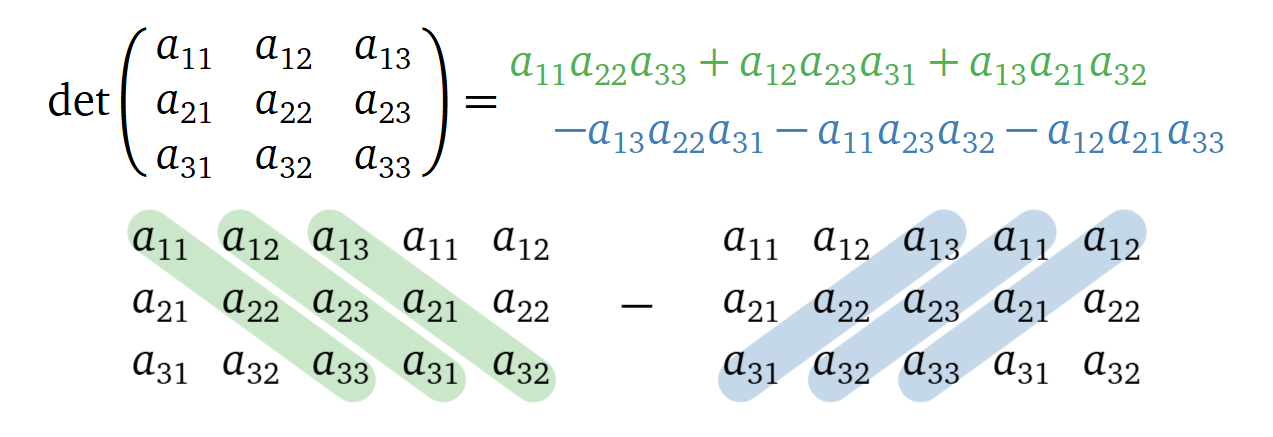
\includegraphics[width=1\linewidth]{detOfA3x3Matrix.png}
    
    \label{fig:det3}
\end{figure}
\end{tcolorbox}

\subsubsection{Cramer’s Rule and Matrix Inverses}

Recall that one can compute the determinant of a \( 2 \times 2 \) matrix using the rule:

\[
A = \begin{pmatrix} a & b \\ c & d \end{pmatrix} \quad \Rightarrow \quad A^{-1} = \frac{1}{\det(A)} \begin{pmatrix} d & -b \\ -c & a \end{pmatrix}.
\]

We computed the cofactors of a \( 2 \times 2 \) matrix as follows: \( C_{11} = d, C_{12} = -c, C_{21} = -b, C_{22} = a \). We can rewrite the formula as:

\[
A^{-1} = \frac{1}{\det(A)} \begin{pmatrix} C_{11} & C_{21} \\ C_{12} & C_{22} \end{pmatrix}.
\]

It turns out that this formula generalizes to \( n \times n \) matrices.

\textbf{Theorem}: Let \( A \) be an invertible \( n \times n \) matrix, with cofactors \( C_{ij} \). Then

\[
A^{-1} = \frac{1}{\det(A)} \begin{pmatrix} 
C_{11} & C_{21} & \cdots & C_{n-1,1} & C_{n1} \\
C_{12} & C_{22} & \cdots & C_{n-1,2} & C_{n2} \\
\vdots & \vdots & \ddots & \vdots & \vdots \\
C_{1,n-1} & C_{2,n-1} & \cdots & C_{n-1,n-1} & C_{n,n-1} \\
C_{1n} & C_{2n} & \cdots & C_{n-1,n} & C_{nn}
\end{pmatrix}.
\]

The matrix of cofactors is sometimes called the adjugate matrix of \( A \), and is denoted \( \text{adj}(A) \):

\[
\text{adj}(A) = \begin{pmatrix} 
C_{11} & C_{21} & \cdots & C_{n-1,1} & C_{n1} \\
C_{12} & C_{22} & \cdots & C_{n-1,2} & C_{n2} \\
\vdots & \vdots & \ddots & \vdots & \vdots \\
C_{1,n-1} & C_{2,n-1} & \cdots & C_{n-1,n-1} & C_{n,n-1} \\
C_{1n} & C_{2n} & \cdots & C_{n-1,n} & C_{nn}
\end{pmatrix}.
\]

Note that the \( (i,j) \)-cofactor \( C_{ij} \) goes in the \( (j,i) \)-entry of the adjugate matrix, not the \( (i,j) \)-entry. Thus, the adjugate matrix is the transpose of the cofactor matrix.

In fact, one always has:

\[
A \cdot \text{adj}(A) = \text{adj}(A) \cdot A = \det(A) I_n,
\]

whether or not \( A \) is invertible.

\paragraph{Example 1:} Compute determinant of \( A^{-1} \)?

Let \( A = \begin{pmatrix} 1 & 0 & 1 \\ 0 & 1 & 1 \\ 1 & 1 & 0 \end{pmatrix} \).

The minors are:

\[
A_{11} = \det \begin{pmatrix} 1 & 1 \\ 1 & 0 \end{pmatrix} = -1, \quad A_{12} = \det \begin{pmatrix} 0 & 1 \\ 1 & 0 \end{pmatrix} = -1, \quad A_{13} = \det \begin{pmatrix} 0 & 1 \\ 1 & 1 \end{pmatrix} = -1,
\]

\[
A_{21} = \det \begin{pmatrix} 0 & 1 \\ 1 & 0 \end{pmatrix} = -1, \quad A_{22} = \det \begin{pmatrix} 1 & 1 \\ 1 & 0 \end{pmatrix} = -1, \quad A_{23} = \det \begin{pmatrix} 1 & 1 \\ 1 & 0 \end{pmatrix} = -1,
\]

\[
A_{31} = \det \begin{pmatrix} 0 & 1 \\ 1 & 1 \end{pmatrix} = -1, \quad A_{32} = \det \begin{pmatrix} 1 & 1 \\ 1 & 0 \end{pmatrix} = -1, \quad A_{33} = \det \begin{pmatrix} 1 & 0 \\ 1 & 1 \end{pmatrix} = -1.
\]

The cofactors are:

\[
C_{11} = -1, \quad C_{12} = 1, \quad C_{13} = -1, \quad C_{21} = 1, \quad C_{22} = -1, \quad C_{23} = -1,
\]

\[
C_{31} = -1, \quad C_{32} = -1, \quad C_{33} = 1.
\]

Expanding along the first row, we compute the determinant:

\[
\det(A) = 1 \cdot C_{11} + 0 \cdot C_{12} + 1 \cdot C_{13} = -2.
\]

Therefore, the inverse is:

\[
A^{-1} = \frac{1}{\det(A)} \begin{pmatrix} C_{11} & C_{21} & C_{31} \\ C_{12} & C_{22} & C_{32} \\ C_{13} & C_{23} & C_{33} \end{pmatrix} = \frac{-1}{2} \begin{pmatrix} -1 & 1 & -1 \\ 1 & -1 & -1 \\ -1 & -1 & 1 \end{pmatrix}.
\]

Thus, the inverse is:

\[
A^{-1} = \begin{pmatrix} 1/2 & -1/2 & 1/2 \\ -1/2 & 1/2 & 1/2 \\ 1/2 & 1/2 & -1/2 \end{pmatrix}.
\]
\begin{tcolorbox}[title=Theorem: Cramer's rule,colframe=blue!70!black, colback=blue!5!white]
Let \( \mathbf{x} = (x_1, x_2, \dots, x_n) \) be the solution of \( A \mathbf{x} = \mathbf{b} \), where \( A \) is an invertible \( n \times n \) matrix and \( \mathbf{b} \) is a vector in \( \mathbb{R}^n \). Let \( A_i \) be the matrix obtained from \( A \) by replacing the \( i \)-th column by \( \mathbf{b} \). Then

\[
x_i = \frac{\det(A_i)}{\det(A)}.
\]

\end{tcolorbox}
\subsubsection{Summary: Methods for Computing Determinants}

There are several methods to compute determinants:

\begin{itemize}
    \item Special formulas for \( 2 \times 2 \) and \( 3 \times 3 \) matrices. This is best for small matrices, except when a \( 3 \times 3 \) matrix has many zeros.
    \item Cofactor expansion. Most efficient when a row or column has zeros, or if the matrix has unknown entries.
    \item Row and column operations. Fastest for large matrices without many zeros.
\end{itemize}

Any combination of these methods can be used. Cofactor expansion is recursive, but the minors can be computed using any convenient method. Row and column operations can also simplify matrices before expanding cofactors.
\begin{tcolorbox}[title=Attention,colframe=blue!70!black, colback=blue!5!white]
$\Rightarrow$ Remember, all methods give the same result for the determinant.
\end{tcolorbox}

\newpage

\subsection{Determinants and Volumes}In this section we give a geometric interpretation of determinants, in terms of volumes.
\subsubsection{Parallelograms and Paralellepipeds}The determinant computes the volume of the following kind of geometric object.

\begin{tcolorbox}[title=Definition,colframe=blue!70!black, colback=blue!5!white]
The parallelepiped determined by \( n \) vectors \( v_1, v_2, \dots, v_n \) in \( \mathbb{R}^n \) is the subset
\[
P = \left\{ a_1 v_1 + a_2 v_2 + \dots + a_n v_n \mid 0 \leq a_1, a_2, \dots, a_n \leq 1 \right\}.
\]

\end{tcolorbox}
In other words, a parallelepiped is the set of all linear combinations of \( n \) vectors with coefficients in \( [0, 1] \). We can draw parallelepipeds using the parallelogram law for vector addition.

\paragraph{Example 1 (The unit cube):}The parallelepiped determined by the standard coordinate vectors \( e_1, e_2, \dots, e_n \) is the unit \( n \)-dimensional cube.

\begin{figure}[H]
    \centering
    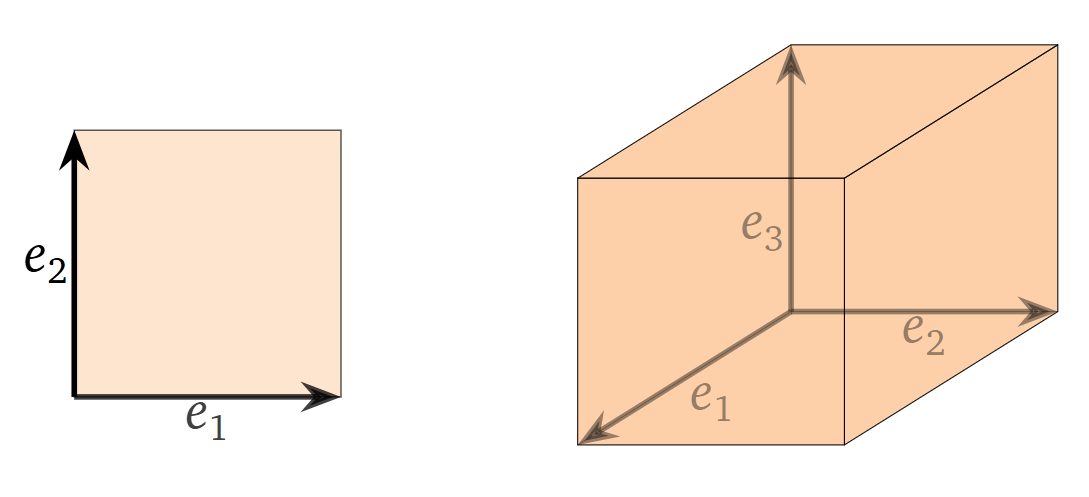
\includegraphics[width=0.5\linewidth]{cubedetage.png}
\end{figure}

\paragraph{Example 2 (Parallelograms):}When \( n = 2 \), a parallelepiped is just a parallelogram in \( \mathbb{R}^2 \). Note that the edges come in parallel pairs.
\begin{figure}[H]
    \centering
    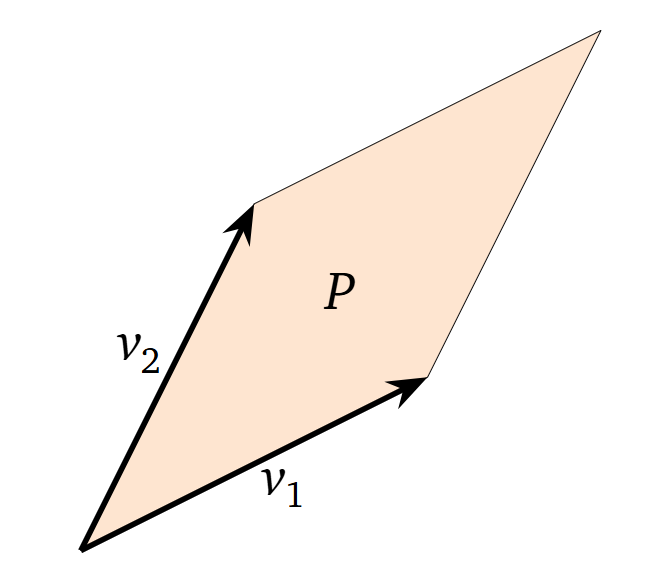
\includegraphics[width=0.5\linewidth]{example2paralellogram.png}
\end{figure}

\paragraph{Example 3 (Parallelepiped):}When \( n = 3 \), a parallelepiped is a kind of skewed cube. Note that the faces come in parallel pairs.
\begin{figure}[H]
    \centering
    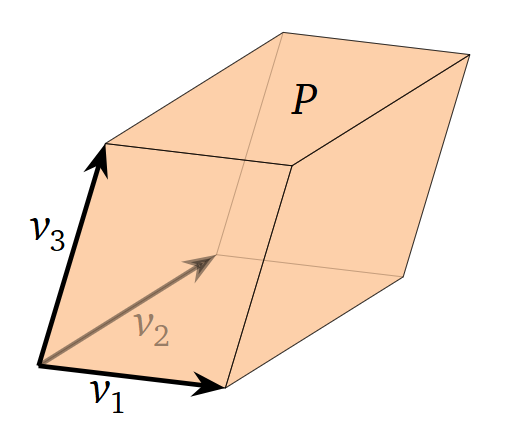
\includegraphics[width=0.5\linewidth]{parallelepiped .png}
\end{figure}
When does a parallelepiped have zero volume? This can happen only if the parallelepiped is flat, i.e., it is squashed into a lower dimension.
\begin{figure}[H]
    \centering
    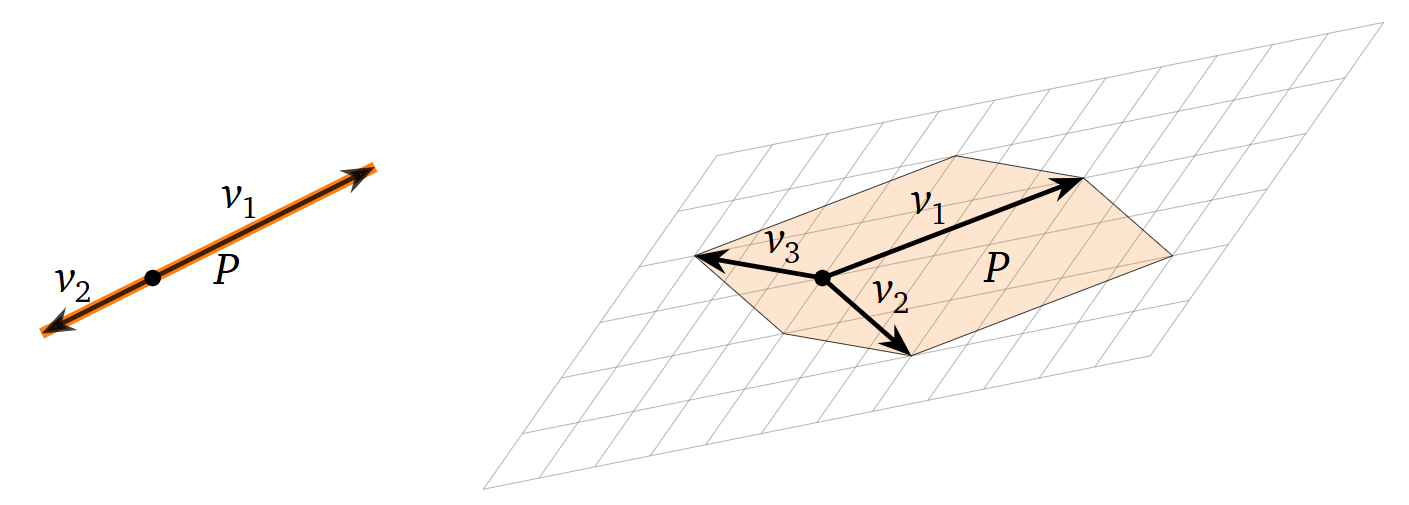
\includegraphics[width=0.75\linewidth]{flat.png}
\end{figure}
This means exactly that \( \{ v_1, v_2, \dots, v_n \} \) is linearly dependent, which by this means that the matrix with rows \( v_1, v_2, \dots, v_n \) has determinant zero. To summarize:

\begin{tcolorbox}[title=Key Observation,colframe=blue!70!black, colback=blue!5!white]
The parallelepiped defined by \( v_1, v_2, \dots, v_n \) has zero volume if and only if the matrix with rows \( v_1, v_2, \dots, v_n \) has zero determinant.
\end{tcolorbox}
\subsubsection{Determinants and Volumes}The key observation above is only the beginning of the story: the volume of a parallelepiped is always a determinant.

\begin{tcolorbox}[title=Theorem(Determinants and volumes),colframe=blue!70!black, colback=blue!5!white]
Let \( v_1, v_2, \dots, v_n \) be vectors in \( \mathbb{R}^n \), let \( P \) be the parallelepiped determined by these vectors, and let \( A \) be the matrix with rows \( v_1, v_2, \dots, v_n \). Then the absolute value of the determinant of \( A \) is the volume of \( P \):
\[
| \det(A) | = \text{vol}(P)
\]
\end{tcolorbox}
\paragraph{Proof:} Since the properties of \ref{def:4propertiesofdeterminant} characterize the determinant, they also characterize the absolute value of the determinant. Explicitly, \( |\det| \) is a function on square matrices that satisfies the following properties:
\begin{itemize}
    \item Doing a row replacement on \( A \) does not change \( |\det(A)| \).
    \item Scaling a row of \( A \) by a scalar \( c \) multiplies \( |\det(A)| \) by \( |c| \).
    \item Swapping two rows of a matrix does not change \( |\det(A)| \).
    \item The determinant of the identity matrix \( I_n \) is equal to \( 1 \).
\end{itemize}

The absolute value of the determinant is the only such function: indeed, by this \ref{def:4propertiesofdeterminant}, if you do some number of row operations on \( A \) to obtain a matrix \( B \) in row echelon form, then
\[
| \det(A) | = \left( \text{product of the diagonal entries of } B \right) \times \left( \text{product of the scaling factors used} \right).
\]
For a square matrix \( A \), we abuse notation and let \( \text{vol}(A) \) denote the volume of the parallelepiped determined by the rows of \( A \). Then we can regard \( \text{vol} \) as a function from the set of square matrices to the real numbers. We will show that \( \text{vol} \) also satisfies the above four properties.


\subsubsection{Volumes of Regions}
\begin{tcolorbox}[title=Definition,colframe=blue!70!black, colback=blue!5!white]
Let \( A \) be an \( n \times n \) matrix with columns \( v_1, v_2, \ldots, v_n \), and let \( T : \mathbb{R}^n \to \mathbb{R}^n \) be the associated matrix transformation \( T(x) = Ax \). Then \( T(e_1) = v_1 \) and \( T(e_2) = v_2 \), so \( T \) takes the unit cube \( C \) to the parallelepiped \( P \) determined by \( v_1, v_2, \ldots, v_n \).
\end{tcolorbox}
\[
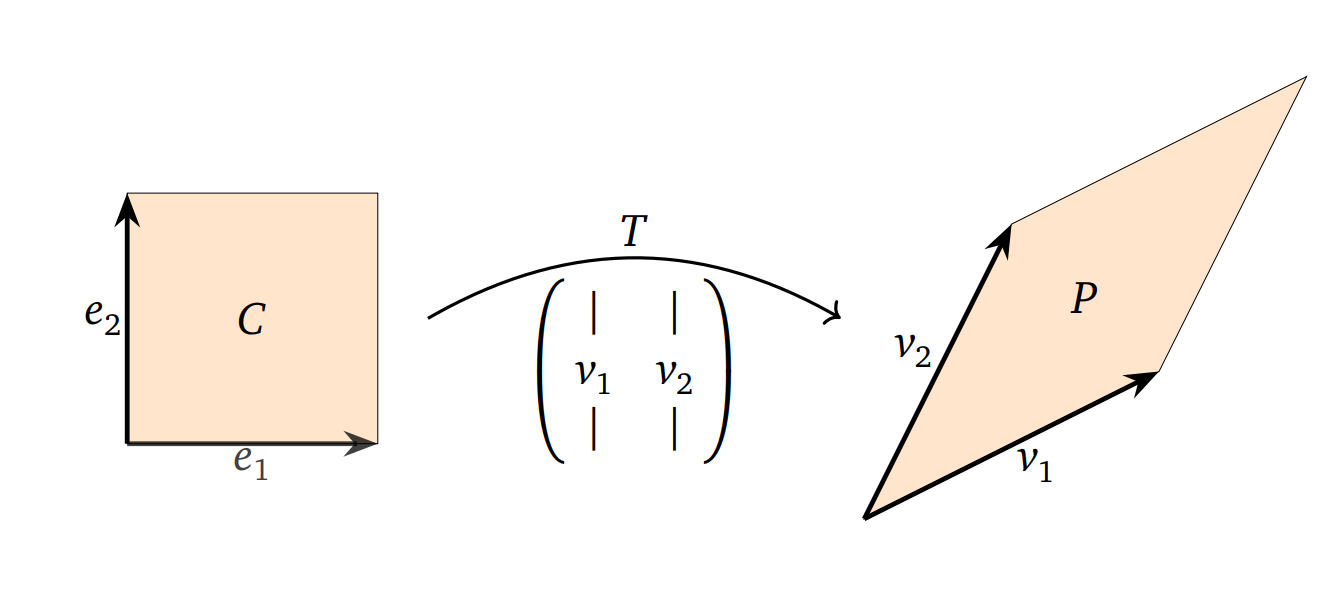
\includegraphics[width=0.8\textwidth]{CtoP.png}
\] 

Since the unit cube has volume 1 and its image has volume \( |\det(A)| \), the transformation \( T \) scaled the volume of the cube by a factor of \( |\det(A)| \). To rephrase:

\begin{tcolorbox}[colback=blue!10, colframe=blue!50, sharp corners=southwest, sharp corners=northeast]
If \( A \) is an \( n \times n \) matrix with corresponding matrix transformation \( T : \mathbb{R}^n \to \mathbb{R}^n \), and if \( C \) is the unit cube in \( \mathbb{R}^n \), then the volume of \( T(C) \) is \( |\det(A)| \).
\end{tcolorbox}

The notation \( T(S) \) means the image of the region \( S \) under the transformation \( T \). In set builder notation, this is the subset

\[
T(S) = \{ T(x) \mid x \in S \}.
\]

In fact, \( T \) scales the volume of \emph{any} region in \( \mathbb{R}^n \) by the same factor, even for curvy regions.

\begin{tcolorbox}[title=Theorem,colframe=blue!70!black, colback=blue!5!white]
Let \( A \) be an \( n \times n \) matrix, and let \( T : \mathbb{R}^n \to \mathbb{R}^n \) be the associated matrix transformation \( T(x) = Ax \). If \( S \) is any region in \( \mathbb{R}^n \), then

\[
\operatorname{vol}(T(S)) = |\det(A)| \cdot \operatorname{vol}(S).
\]
\end{tcolorbox}
\subparagraph{Proof.} Let \( C \) be the unit cube, let \( v_1, v_2, \ldots, v_n \) be the columns of \( A \), and let \( P \) be the parallelepiped determined by these vectors, so \( T(C) = P \) and \( \operatorname{vol}(P) = |\det(A)| \). For \( \varepsilon > 0 \), let \( \varepsilon C \) be the cube with side lengths \( \varepsilon \), i.e., the parallelepiped determined by the vectors \( \varepsilon e_1, \varepsilon e_2, \ldots, \varepsilon e_n \), and we define \( \varepsilon P \) similarly. By the second derivative property, \( T \) takes \( \varepsilon C \) to \( \varepsilon P \). The volume of \( \varepsilon S \) (we've scaled each of the \( n \) standard vectors by a factor of \( \varepsilon \)) and the volume of \( \varepsilon P \) is \( |\det(A)| \cdot \varepsilon^n \) (for the same reason), so we have shown that \( T \) scales the volume of \( \varepsilon C \) by \( |\det(A)| \).

By the first \textit{defining property}, the image of a translation of \( \varepsilon C \) is simply a translation of \( \varepsilon P \):

\[
T(x + \varepsilon C) = T(x) + \varepsilon T(C) = T(x) + \varepsilon P.
\]

Since translations don't affect volume, this shows that \( T \) scales the volume of \( \varepsilon C \) by \( |\det(A)| \).

At this point, we rely on multivariable calculus for the rest of the argument. The idea is that any region \( S \) can be closely approximated by small cubes of the form \( x + \varepsilon C \). The image \( T(S) \) can then be approximated by the collection of images of these cubes, each of which takes the form \( T(x) + \varepsilon P \).

\[
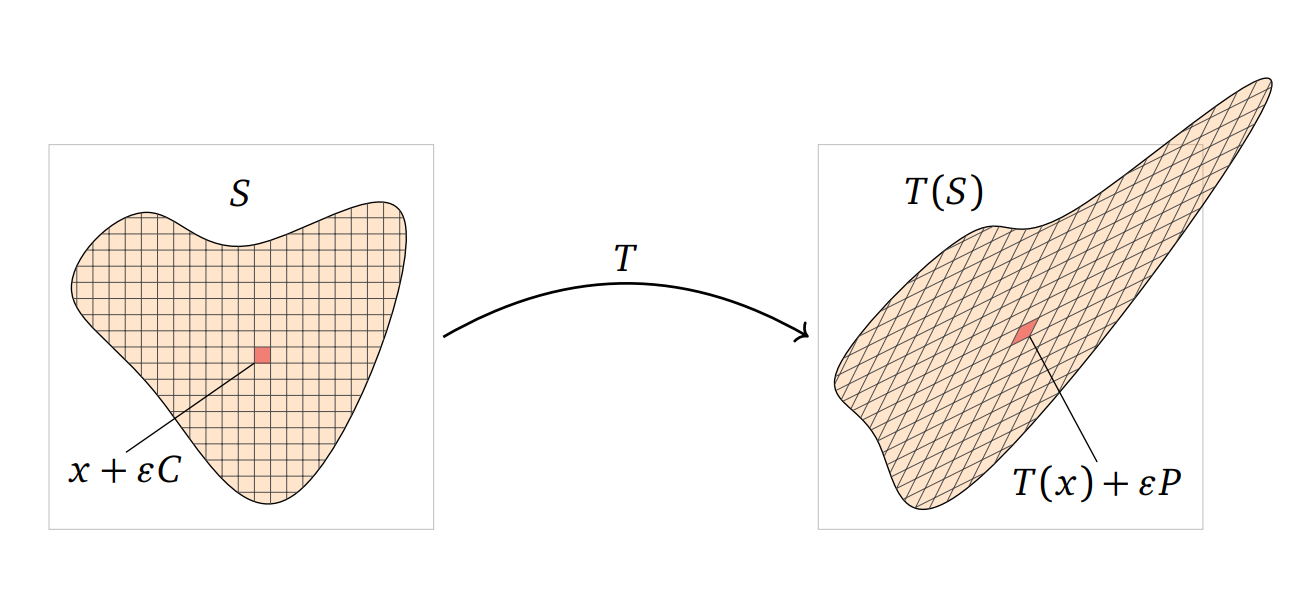
\includegraphics[width=0.9\textwidth]{StoT.png}
\]

The volume of \( S \) is roughly the sum of the volumes of these cubes. When \( \varepsilon \) approaches zero, this approximation becomes exact. Therefore, the volume of \( T(S) \) can be calculated as the sum of the volumes of the parallelepipeds, taking the limit as \( \varepsilon \to 0 \).

The key point here is that the volume of each small cube gets scaled by \( |\det(A)| \). So, the total volume of the parallelepipeds is \( |\det(A)| \) times the total volume of the cubes. This leads to the conclusion:

\[
\operatorname{vol}(T(S)) = |\det(A)| \cdot \operatorname{vol}(S).
\]

\paragraph{Example (Area of an ellipse):}Find the are of the interior $E$ of the ellipse defined by the equation

\paragraph{Example.} Let \( S \) be a half-circle of radius 1, and let

\[
A = \begin{pmatrix} 1 & 2 \\ 2 & 1 \end{pmatrix}.
\]

We define a linear transformation \( T: \mathbb{R}^2 \to \mathbb{R}^2 \) by \( T(x) = Ax \). The question is: what is the area of \( T(S) \)?

\[
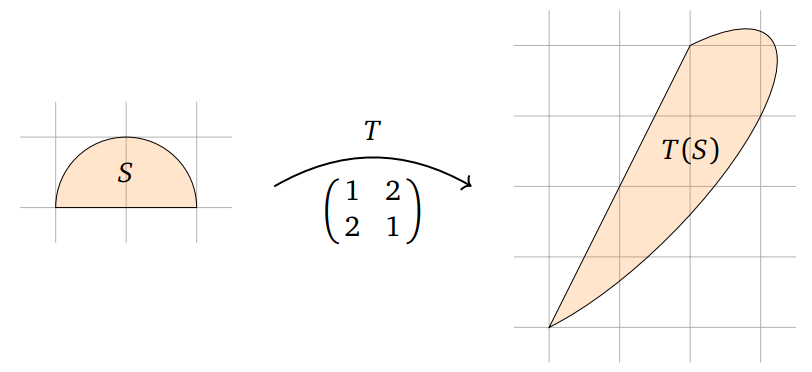
\includegraphics[width=0.9\textwidth]{lineartrans.png}
\]

\textbf{Solution.} The area of the original unit half-circle \( S \) is \( \pi/2 \). The transformation \( T \) scales the area by a factor of \( |\det(A)| \). Since

\[
\det(A) = \det\begin{pmatrix} 1 & 2 \\ 2 & 1 \end{pmatrix} = 1 \cdot 1 - 2 \cdot 2 = -3,
\]

we have \( |\det(A)| = 3 \). Therefore, the area of \( T(S) \) is:

\[
\operatorname{vol}(T(S)) = 3 \cdot \frac{\pi}{2} = \frac{3\pi}{2}.
\]

\paragraph{Example (Area of an ellipse).} Find the area of the interior \( E \) of the ellipse defined by the equation:

\[
\left(\frac{x - y}{2}\right)^2 + \left(\frac{x + 3y}{3}\right)^2 = 1.
\]

\textbf{Solution.} This ellipse can be obtained from the unit circle \( x^2 + y^2 = 1 \) by applying the following linear transformation:

\[
A = \frac{2x - y}{2}, \quad B = \frac{y + 3x}{3}.
\]

Alternatively, in matrix form, we can express this transformation as:

\[
T\left(\begin{pmatrix} A \\ B \end{pmatrix}\right) = \begin{pmatrix} \frac{2x - y}{2} \\ \frac{y + 3x}{3} \end{pmatrix}.
\]

This means \( T(z, y) \) lies on the unit circle if and only if \( (z, y) \) lies on the ellipse \( E \).

\[
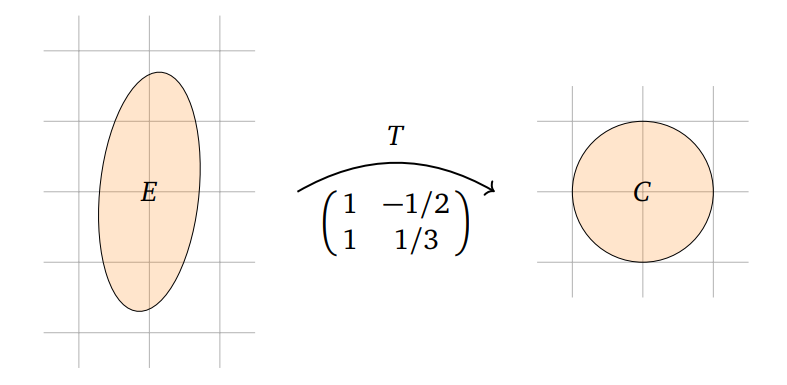
\includegraphics[width=0.9\textwidth]{EtoC.png}
\]

The transformation \( T \) scales the area by \( |\det(A)| \), where \( A \) is the corresponding matrix. This gives us the area of the ellipse \( E \) as the scaled area of the unit circle.

Alternatively, in matrix form, we express the transformation \( T \) as:

\[
T\left(\begin{pmatrix} x \\ y \end{pmatrix}\right) = \begin{pmatrix} \frac{2x - y}{2} \\ \frac{x + 3y}{3} \end{pmatrix}.
\]

This means \( T(A, B) \) lies on the unit circle if and only if \( (A, B) \) lies on the ellipse \( E \).

The transformation \( T \) scales the area by a factor of \( |\det(A)| \), where \( A \) is the corresponding matrix for \( T \). We write \( A \) explicitly as:

\[
\ A = 
\begin{pmatrix}
1 & -\frac{1}{2} \\
1 & \frac{1}{3}
\end{pmatrix}
\]

The determinant of \( A \) is:

\[
\det(A) = \begin{vmatrix} 1 & -\frac{1}{2} \\
1 & \frac{1}{3} \end{vmatrix} = \frac{5}{6}.
\]

Since the area of the unit circle is \( \pi \), the area of the ellipse \( E \) is scaled by \( |\det(A)| \):

\[
\text{Area of } E = |\det(A)| \cdot \text{Area of unit circle} = \frac{6}{5} \cdot \pi = \frac{6\pi}{5}.
\]

Thus, the area of the ellipse \( E \) is:

\[
\boxed{\frac{6\pi}{5}.}
\]

---

\paragraph{Remark (Multiplicativity of \( |\det| \)).} The above result highlights an important property of determinants: their multiplicative nature. Suppose \( A \) and \( B \) are \( n \times n \) matrices, and \( T, U: \mathbb{R}^n \to \mathbb{R}^n \) are the corresponding linear transformations. If \( C \) represents the unit cube, then the volume transformation follows this logic:

\[
\text{vol}(T \circ U(C)) = \text{vol}(T(U(C))) = |\det(A)| \cdot \text{vol}(U(C)).
\]

We know that \( \text{vol}(U(C)) \) itself scales by \( |\det(B)| \), so:

\[
\text{vol}(T \circ U(C)) = |\det(A)| \cdot |\det(B)| \cdot \text{vol}(C).
\]

On the other hand, the matrix of the composition \( T \circ U \) is precisely the product \( AB \), which also scales the volume. Thus:

\[
\text{vol}(T \circ U(C)) = |\det(AB)| \cdot \text{vol}(C).
\]

Combining these results, we obtain the key property:

\[
|\det(AB)| = |\det(A)| \cdot |\det(B)|.
\]

This property ensures that determinants are multiplicative, reinforcing their fundamental role in linear transformations and volume scaling.


\newpage
\Large \section{Eigenvalue and Eigenvector}
\large \subsection{The definitions of Eigenvalue and Eigenvector}
\small \subsubsection{Eigenvalues and Eigenvector}
\begin{frame}
    

\small


\small At this part, we will answer the question: What is \textbf{eigenvalue} and \textbf{eigenvector}?

Firstly, we need to remember that definition:


\begin{tcolorbox}[title=Definition,colframe=blue!70!black, colback=blue!5!white]
Let \(A\) be an \(n \times n\) matrix:
\begin{itemize}
    \item An \textbf{eigenvalue} of \(A\) is a \textit{nonzero} vector v in \(R^n\) such that \(Av=\lambda v\), for some scalar \(\lambda\).
    \item An \textbf{eigenvector} of \(A\) is a scalar \(\lambda\) such that the equation \(Ax =  \lambda x\)  has \textit{nontrivial} solution.
\end{itemize}

    If \(Av = \lambda v\), \(v \neq 0\), we say that \(\lambda\) is the \textbf{eigenvalue} for \(v\), and \(v\) is an \textbf{eigenvector} for \(\lambda\).
\end{tcolorbox}
\paragraph{Note:}
    With the equation \(Av = \lambda v\)
    \begin{itemize}
        \item \(A\) is an \(n \times n\) matrix
        \item \(v\) is an \(1 \times n\) matrix
        \item \(\lambda\) is an scalar
    \end{itemize}

    For the multiplication \(Av\) to make sense, \(A\) must be a square matrix, as it maps the vector \(v\) from space \(R^n\) back to same space \(R^n\).

    An eigenvector is always nonzero, but an eigenvalue can be zero. In the equation \(A\mathbf{v} = \lambda \mathbf{v}\), \(\lambda\) can be zero for some nonzero \(\mathbf{v}\). However, if \(\mathbf{v} = 0\), any \(\lambda \in \mathbb{R}\) would satisfy the equation, making the case trivial and thus excluded.

    \paragraph{} So, how to find the eigenvalue with eigenvector \(v\)? The solution is so simple, just multiply the matrix \(A\) with vector \(v\), and check that answer is a multiplication of \(v\) or not. If it's true, we can find \(\lambda\) easily. Let see it in example. 

\paragraph{Example} Find the eigenvalue with:
\[       
    A = 
    \left(
    \begin{array}{cc}
    2 & 2 \\
    -4 & 8
    \end{array}
    \right)
    ; v =
    \left(
    \begin{array}{c}
    1 \\
    1
    \end{array}
    \right)
    ; w = 
    \left(
    \begin{array}{c}
    2 \\
    1
    \end{array}
    \right)
\]

What are eigenvectors? What are their eigenvalues?
\paragraph{Solution} We have:
\[       
    Av = 
    \left(
    \begin{array}{cc}
    2 & 2 \\
    -4 & 8
    \end{array}
    \right)
    \left(
    \begin{array}{c}
    1 \\
    1
    \end{array}
    \right)
    = 
    \left(
    \begin{array}{c}
    4 \\
    4
    \end{array}
    \right)
    = 4v
\]

Hence, \(v\) is an eigenvector of A, with eigenvalue \(\lambda=4\). On the other hand,

\[       
    Av = 
    \left(
    \begin{array}{cc}
    2 & 2 \\
    -4 & 8
    \end{array}
    \right)
    \left(
    \begin{array}{c}
    2 \\
    1
    \end{array}
    \right)
    = 
    \left(
    \begin{array}{c}
    6 \\
    0
    \end{array}
    \right)
\]

which is not a scalar multiple of \(w\). Hence, \(w\) is not an eigenvector of A.
\newpage

Geometrically, we can understand that Eigenvectors are vectors that, when transformed by \( A \), remain on the same straight line through the origin. On the other hand, Eigenvalues are scalars that represent the degree of stretching or rotation of the Eigenvectors. This is particularly useful for certain fixed vectors, as instead of storing the complex matrix \( A \), we only need to store the simple \( \lambda \), which saves memory.
\paragraph{Properties}
\begin{itemize}
    \item Eigenvectors corresponding to different eigenvalues are always \textit{linearly independent}.
    
    Let A be an \(n \times n\) matrix, \(v_1, v_2, v_3,..., v_n\) linear combination of eigenvectors \(v_1, v_2, v_3,..., v_n\) and coefficients \(c_1, c_2, c_3,...,c_n\) that:
    \[v_1c_1 + v_2c_2+...+v_nc_n=0\]
    Multiply both sides by matrix A:
    \[\Longleftrightarrow A(v_1c_1 + v_2c_2+...+v_nc_n)=0\]
    \(Av_i = \lambda_iv_i\) with \(\lambda_i\) is the eigenvalue with eigenvector \(v_i\) 
    \[\Longleftrightarrow \lambda_1v_1c_1 + \lambda_2v_2c_2+...+\lambda_nv_nc_n=0\]
    Because the eigenvectors are distinct, the coefficients \(c_1, c_2, ..., c_n\) must be all zero, proving that the eigenvectors are linearly independent.  
    \item A matrix of size \(n \times n\) can have at most \(n\) eigenvalues.

    For a matrix belonging to the space \(\mathbb{R}^n\), we can think of that matrix as being similar to a vector in the same space. The eigenvectors in this space can be seen as the axes of a coordinate system, and we can represent the matrix in a manner similar to representing a vector in a coordinate system using eigenvalues. Since the space is \(\mathbb{R}^n\), we can have at most \(n\) eigenvalues.

\end{itemize}
\end{frame}
\small \subsubsection{Eigenspaces}
\begin{frame}
\small

\small We already know how to determine the eigenvalue from a given eigenvector. Our next goal is, given a matrix \(A\) and an eigenvalue \(\lambda\), to find the eigenvector that satisfies the equation \(Ax = \lambda x\).

Let's see the equation:

\[
Ax=\lambda v
\]
\[
\Longleftrightarrow
Ax - \lambda v = 0
\]
\[
\Longleftrightarrow
Ax - \lambda I_n v = 0
\]
\[
\Longleftrightarrow
(A - \lambda I_n)v = 0
\]
\newpage
Therefore, the eigenvector with eigenvalue \(\lambda\), if any, are the nontrivial solution of the equation \((A-\lambda I_n)v=0\). If the equation has no nontrivial solution, \(\lambda\) is not an eigenvalue of \(A\).



\begin{tcolorbox}[title=Definition,colframe=blue!70!black, colback=blue!5!white]
Let \( A \) be an \( n \times n \) matrix, and let \( \lambda \) be an eigenvalue of \( A \). The eigenspace of \( A \) is the solution set of \( (A - \lambda I)v = 0 \), i.e., the subspace \( \text{Nul}(A - \lambda I) \).
\end{tcolorbox}
\paragraph{Example}. (Computing eigenspaces): 

For each of the numbers \( \lambda = 2, 1, 3 \), decide if \( \lambda \) is an eigenvalue of the matrix

\[
A = \begin{pmatrix}
2 & -4 \\
-1 & -1
\end{pmatrix}
\]

and if so, compute a basis for the \( \lambda \)-eigenspace.

\paragraph{Solution}: 

The number \( 3 \) is an eigenvalue of \( A \) if and only if \( \text{Nul}(A - 3I_2) \) is nonzero. Hence, we have to solve the matrix equation \( (A - 3I_2)v = 0 \). We compute \( A - 3I_2 \):

\[
A - 3I_2 = \begin{pmatrix}
2 & -4 \\
-1 & -1
\end{pmatrix} - \begin{pmatrix}
3 & 0 \\
0 & 3
\end{pmatrix}
= \begin{pmatrix}
-1 & -4 \\
-1 & -4
\end{pmatrix}
\]

Next, we reduce this matrix to row echelon form:

\[
\begin{pmatrix}
1 & 4 \\
0 & 0
\end{pmatrix}
\]

From this, we can write the system of equations:

\[
x = -4y, \quad y = y
\]

In parametric vector form, we have:

\[
\begin{pmatrix}
x \\
y
\end{pmatrix} = y \begin{pmatrix} 4 \\ 1 \end{pmatrix}
\]

Since \( y \) is a free variable, the null space of \( A - 3I_2 \) is nonzero, so \( 3 \) is an eigenvalue. A basis for the \( 3 \)-eigenspace is:

\[
\left\{ \begin{pmatrix} -4 \\ 1 \end{pmatrix} \right\}
\]

Concretely, we have shown that the eigenvectors of \( A \) with eigenvalue \( 3 \) are exactly the nonzero multiples of \( \begin{pmatrix} -4 \\ 1 \end{pmatrix} \). In particular, \( \begin{pmatrix} -4 \\ 1 \end{pmatrix} \) is an eigenvector, which we can verify:

\[
A \begin{pmatrix} -4 \\ 1 \end{pmatrix} = \begin{pmatrix} 2 & -4 \\ -1 & -1 \end{pmatrix} \begin{pmatrix} -4 \\ 1 \end{pmatrix} = \begin{pmatrix} -12 \\ 3 \end{pmatrix} = 3 \begin{pmatrix} -4 \\ 1 \end{pmatrix}
\]

The number \( 1 \) is an eigenvalue of \( A \) if and only if \( \text{Nul}(A - I_2) \) is nonzero. Hence, we have to solve the matrix equation \( (A - I_2)v = 0 \). We compute \( A - I_2 \):

\[
A - I_2 = \begin{pmatrix}
2 & -4 \\
-1 & -1
\end{pmatrix} - \begin{pmatrix}
1 & 0 \\
0 & 1
\end{pmatrix}
= \begin{pmatrix}
1 & 4 \\
1 & 0
\end{pmatrix}
\]

The determinant of this matrix is \( 6 \), so it is invertible. By the invertible matrix theorem, we have \( \text{Nul}(A - I_2) = 0 \), so \( 1 \) is not an eigenvalue.

The eigenvectors of \( A \) with eigenvalue \( 2 \), if any, are the nonzero solutions of the matrix equation \( (A + 2I_2)v = 0 \). We have:

\[
A + 2I_2 = \begin{pmatrix}
2 & 4 \\
1 & 1
\end{pmatrix} + \begin{pmatrix}
2 & 0 \\
0 & 2
\end{pmatrix}
= \begin{pmatrix}
4 & -4 \\
-1 & 1
\end{pmatrix}
\]

We reduce this matrix to row echelon form:

\[
\begin{pmatrix}
1 & -1 \\
0 & 0
\end{pmatrix}
\]

In parametric form, we have:

\[
x = y, \quad y = y
\]

In parametric vector form:

\[
\begin{pmatrix}
x \\
y
\end{pmatrix} = y \begin{pmatrix} 1 \\ 1 \end{pmatrix}
\]

Hence, there exist eigenvectors with eigenvalue \( 2 \), namely, any nonzero multiple of \( \begin{pmatrix} 1 \\ 1 \end{pmatrix} \). A basis for the \( 2 \)-eigenspace is:

\[
\left\{ \begin{pmatrix} 1 \\ 1 \end{pmatrix} \right\}
\]
\paragraph{Properties}
\begin{itemize}
    \item If \(\lambda\) is an eigenvalue, its eigenspace contains infinitely many eigenvectors (every vector is a scalar multiple of the original eigenvector).
    \item The dimension of the eigenspace is equal to the number of free variables in the system of equations\((A - \lambda I_n)v = 0.\).(Easily prove by the properties of eigenvector).
\end{itemize}

\paragraph{Recipes}

Let \( A \) be an \( n \times n \) matrix and let \( \lambda \) be a number.

\begin{enumerate}
    \item \( \lambda \) is an eigenvalue of \( A \) if and only if \( (A - \lambda I_n)v = 0 \) has a nontrivial solution, which is equivalent to \( \text{Nul}(A - \lambda I_n) \neq \{0\} \).
    
    \item In this case, finding a basis for the \( \lambda \)-eigenspace of \( A \) means finding a basis for \( \text{Nul}(A - \lambda I_n) \). This can be done by solving \( (A - \lambda I_n)v = 0 \) and expressing the solutions in parametric vector form.
    
    \item The dimension of the \( \lambda \)-eigenspace of \( A \) is equal to the number of free variables in the system of equations \( (A - \lambda I_n)v = 0 \), which corresponds to the number of columns of \( A - \lambda I_n \) without pivots.
    
    \item The eigenvectors with eigenvalue \( \lambda \) are the nonzero vectors in \( \text{Nul}(A - \lambda I_n) \), or equivalently, the nontrivial solutions of \( (A - \lambda I_n)v = 0 \).
\end{enumerate}

\end{frame}

\small \subsubsection{The Inverible Matrix Theorem: Addenda}
\begin{frame}
    \small

    \small We now have two new ways of saying that a matrix is invertible, so we add them to the invertible matrix theorem.

\textbf{Invertible Matrix Theorem.} Let \( A \) be an \( n \times n \) matrix, and let \( T: \mathbb{R}^n \to \mathbb{R}^n \) be the matrix transformation \( T(x) = Ax \). The following statements are equivalent:

\begin{enumerate}
    \item \( A \) is invertible.
    \item \( A \) has \( n \) pivots.
    \item \( \text{Nul}(A) = \{0\} \).
    \item The columns of \( A \) are linearly independent.
    \item The columns of \( A \) span \( \mathbb{R}^n \).
    \item \( Ax = b \) has a unique solution for each \( b \) in \( \mathbb{R}^n \).
    \item \( T \) is invertible.
    \item \( T \) is one-to-one.
    \item \( T \) is onto.
    \item \( \det(A) \neq 0 \).
    \item \( 0 \) is not an eigenvalue of \( A \).
\end{enumerate}
\end{frame}

\Large \subsection{The Characteristic Polynomial}
\begin{frame}
\small

\small In the previous subsection, we learned how to find the eigenvector for a given eigenvalue. Now, the question is: how do we find the eigenvalues?

\begin{tcolorbox}[title=Definition,colframe=blue!70!black, colback=blue!5!white]
Let \( A \) be an \( n \times n \) matrix.
\begin{enumerate}
    \item The \textbf{characteristic polynomial} of \( A \) is the function \( f(\lambda) \) defined as:
    \[
    f(\lambda) = \det(A - \lambda I_n)
    \]
    \item A number \( \lambda \) is called an \textit{eigenvalue} of \( A \) if \( f(\lambda) = 0 \).
\end{enumerate}
\end{tcolorbox}
Now, we prove it.

\[
\begin{array}{lcl}
    \lambda \text{ is an eigenvalue of A} & \implies & Ax = \lambda x \text{ has a nontrivial solution,} \\
    &\implies &(A - \lambda I_n)x = 0 \text{ has a nontrivial solution.} \\
    &\implies &A - \lambda I_n \text{ is not invertible.} \\
    &\implies & \det(A - \lambda I_n) = 0.               \\
    &\implies & f(\lambda) = 0.               \\
\end{array}
\]

\newpage
\paragraph{Example: Finding Eigenvalues and Eigenvectors}

Let 
\[
A = \begin{pmatrix} 3 & 2 \\ 4 & 1 \end{pmatrix}.
\]
\paragraph{Solution} 

\[\]

\textbf{Characteristic Polynomial}

\small

The characteristic polynomial is:
\[
f(\lambda) = \det(A - \lambda I_2) = \det\begin{pmatrix} 3-\lambda & 2 \\ 4 & 1-\lambda \end{pmatrix}.
\]

Expanding the determinant:
\[
f(\lambda) = (3-\lambda)(1-\lambda) - (4)(2),
\]
\[
f(\lambda) = \lambda^2 - 4\lambda - 5.
\]

\textbf{Finding Eigenvalues}

To find the eigenvalues, solve \( f(\lambda) = 0 \):
\[
\lambda^2 - 4\lambda - 5 = (\lambda - 5)(\lambda + 1) = 0.
\]

Thus, the eigenvalues are:
\[
\lambda_1 = 5 \quad \text{and} \quad \lambda_2 = -1.
\]

\textbf{Finding Eigenvectors}

Solve \( (A - \lambda I_2)v = 0 \) for each eigenvalue.

\textbf{For \( \lambda_1 = 5 \):}
\[
A - 5I_2 = \begin{pmatrix} 3-5 & 2 \\ 4 & 1-5 \end{pmatrix} = \begin{pmatrix} -2 & 2 \\ 4 & -4 \end{pmatrix}.
\]

The system of equations is:
\[
-2x + 2y = 0, \quad 4x - 4y = 0.
\]

Simplifying:
\[
x = y.
\]

Thus, the eigenvector corresponding to \( \lambda_1 = 5 \) is:

\[
v_1 = \begin{pmatrix} 1 \\ 1 \end{pmatrix}.
\]

\textbf{}{For \( \lambda_2 = -1 \):}
\[
A - (-1)I_2 = A + I_2 = \begin{pmatrix} 3+1 & 2 \\ 4 & 1+1 \end{pmatrix} = \begin{pmatrix} 4 & 2 \\ 4 & 2 \end{pmatrix}.
\]

The system of equations is:

\[
4x + 2y = 0, \quad 4x + 2y = 0.
\]

Simplifying:

\[
2x + y = 0 \quad \Rightarrow \quad y = -2x.
\]

Thus, the eigenvector corresponding to \( \lambda_2 = -1 \) is:

\[
v_2 = \begin{pmatrix} 1 \\ -2 \end{pmatrix}.
\]

\textbf{Final Results}
\begin{itemize}
    \item \textbf{Eigenvalues:} \( \lambda_1 = 5 \), \( \lambda_2 = -1 \).
    \item \textbf{Eigenvectors:}
    \begin{itemize}
        \item For \( \lambda_1 = 5 \): \( v_1 = \begin{pmatrix} 1 \\ 1 \end{pmatrix} \).
        \item For \( \lambda_2 = -1 \): \( v_2 = \begin{pmatrix} 1 \\ -2 \end{pmatrix} \).
    \end{itemize}
\end{itemize}
\
\end{frame}


\Large \subsection{Similarity}\label{sec:Similarity}
\small

\small

Some matrices are easy to understand. For instance, a diagonal matrix 
\[
D = \begin{pmatrix} 2 & 0 \\ 0 & \frac{1}{2} \end{pmatrix}
\]
just scales the coordinates of a vector:
\[
D \begin{pmatrix} x \\ y \end{pmatrix} = \begin{pmatrix} 2x \\ \frac{y}{2} \end{pmatrix}.
\]
The purpose of most of the rest of this chapter is to understand complicated-looking matrices by analyzing to what extent they “behave like” simple matrices. For instance, the matrix
\[
A = \begin{pmatrix} 1 & 1 \\ 6 & 9 \end{pmatrix}
\]
has eigenvalues \(2\) and \(\frac{1}{2}\), with corresponding eigenvectors 
\[
v_1 = \begin{pmatrix} \frac{2}{3} \\ 1 \end{pmatrix}, \quad v_2 = \begin{pmatrix} -1 \\ 1 \end{pmatrix}.
\]
Notice that
\[
D(xe_1 + ye_2) = xDe_1 + yDe_2 = \begin{pmatrix} 2x \\ -\frac{1}{2}y \end{pmatrix},
\]
and
\[
A(xv_1 + yv_2) = xAv_1 + yAv_2 = \begin{pmatrix} 2x \\ -\frac{1}{2}y \end{pmatrix}.
\]
Using \(v_1, v_2\) instead of the usual coordinates makes \(A\) “behave” like a diagonal matrix.

In this section, we study in detail the situation when two matrices behave similarly with respect to different coordinate systems.

\subsubsection{Similar Matrices}
        \begin{tcolorbox}[title=Definition,colframe=blue!70!black, colback=blue!5!white]
    Two \(n \times n\) matrices \(A\) and \(B\) are \textit{similar} if there exists an invertible \(n \times n\) matrix \(C\) such that 
\[
A = C B C^{-1}.
\]

        \end{tcolorbox}

\paragraph{Proposition:}Let \(A\), \(B\), and \(C\) be \(n \times n\) matrices. The following properties hold:
\subparagraph{Proof:}Taking \(C = I_n = I_n^{-1}\), we have 
\[
A = I_n A I_n^{-1}.
\]

Suppose that \(A = C B C^{-1}\). Multiplying both sides on the left by \(C^{-1}\) and on the right by \(C\) gives
\[
C^{-1} A C = C^{-1} (C B C^{-1}) C = B.
\]

Since \((C^{-1})^{-1} = C\), we have 
\[
B = C^{-1} A (C^{-1})^{-1},
\]
so that \(B\) is similar to \(A\).

Suppose that \(A = D B D^{-1}\) and \(B = E C E^{-1}\). Substituting for \(B\) and remembering that \((DE)^{-1} = E^{-1} D^{-1}\), we have
\[
A = D (E C E^{-1}) D^{-1} = (DE) C (DE)^{-1},
\]
which shows that \(A\) is similar to \(C\).

\paragraph{Fact:}Let \(A = C B C^{-1}\). Then, for any \(n \geq 1\), we have
\[
A^n = C B^n C^{-1}.
\]

\subparagraph{Proof:}First, note that 
\[
A^2 = A A = (C B C^{-1})(C B C^{-1}) = C B (C^{-1} C) B C^{-1} = C B I_n B C^{-1} = C B^2 C^{-1}.
\]

Next, we have
\[
A^3 = A^2 A = (C B^2 C^{-1})(C B C^{-1}) = C B^2 (C^{-1} C) B C^{-1} = C B^3 C^{-1}.
\]

The pattern is clear.
\subsubsection{Eigenvalues of Similar Matrices}Since similar matrices behave in the same way with respect to different coordinate systems, we should expect their eigenvalues and eigenvectors to be closely related.
\begin{tcolorbox}[title=Fact,colframe=blue!70!black, colback=blue!5!white]
\textit{Similar matrices have the same characteristic polynomial.}
\end{tcolorbox}
\subparagraph{Proof:}Suppose that \( A = CBC^{-1} \), where \( A \), \( B \), and \( C \) are \( n \times n \) matrices. We calculate
\[
A - \lambda I_n = CBC^{-1} - \lambda I_n = C(B - \lambda I_n)C^{-1}.
\]
Therefore, 
\[
\det(A - \lambda I_n) = \det(C(B - \lambda I_n)C^{-1}) = \det(C) \det(B - \lambda I_n) \det(C^{-1}) = \det(B - \lambda I_n).
\]

\newpage
\subsection{Diagonalization}Diagonal matrices are the easiest kind of matrices to understand: they just scale the coordinate directions by their diagonal entries. In \ref{sec:Similarity}, we saw that similar matrices behave in the same way, with respect to different coordinate systems. Therefore, if a matrix is similar to a diagonal matrix, it is also relatively easy to understand. This section is devoted to the question: “When is a matrix similar to a diagonal matrix?”

\begin{tcolorbox}[title=Definition,colframe=blue!70!black, colback=blue!5!white]
An \(n \times n\) matrix \(A\) is \textit{diagonalizable} if it is similar to a diagonal matrix: that is, if there exists an invertible \(n \times n\) matrix \(C\) and a diagonal matrix \(D\) such that
\[
A = C D C^{-1}.
\]

\end{tcolorbox}

\paragraph{Powers of diagonalizable matrices}Multiplying diagonal matrices together just multiplies their diagonal entries:

\[
\begin{pmatrix}
    x_1 & 0 & 0\\
    0 & x_2 & 0\\
    0 & 0 & x_3
\end{pmatrix}
\begin{pmatrix}
    y_1 & 0 & 0\\
    0 & y_2 & 0\\
    0 & 0 & y_3
\end{pmatrix} = 
\begin{pmatrix}
    x_1y_1 & 0 & 0\\
    0 & x_2y_2 & 0\\
    0 & 0 & x_3y_3
\end{pmatrix}
\]
Therefore, it is easy to take powers of a diagonal matrix:
\[
\begin{pmatrix}
    x & 0 & 0\\
    0 & y & 0\\
    0 & 0 & z
\end{pmatrix}^n = \begin{pmatrix}
    x^n & 0 & 0\\
    0 & y^n & 0\\
    0 & 0 & z^n
\end{pmatrix}
\]

\begin{tcolorbox}[title=Recipe: Compute powers of a diagonalizable matrix,colframe=blue!70!black, colback=blue!5!white]
If \( A = C D C^{-1} \), where \(D\) is a diagonal matrix, then
\[
A^n = C D^n C^{-1}.
\]
Specifically, for the matrix \(A\),
\[
A = C \begin{pmatrix} x & 0 & 0 \\ 0 & y & 0 \\ 0 & 0 & z \end{pmatrix} C^{-1}
\quad \Rightarrow \quad
A^n = C \begin{pmatrix} x^n & 0 & 0 \\ 0 & y^n & 0 \\ 0 & 0 & z^n \end{pmatrix} C^{-1}.
\]
\end{tcolorbox}
A fundamental question about a matrix is whether or not it is diagonalizable. The following is the primary criterion for diagonalizability. It shows that diagonalizability is an eigenvalue problem.

\begin{tcolorbox}[title=Diagonalization Theorem,colframe=blue!70!black, colback=blue!5!white]
An \(n \times n\) matrix \(A\) is diagonalizable if and only if \(A\) has \(n\) linearly independent eigenvectors. In this case, 
\[
A = C D C^{-1}
\]
for 
\[
C = \begin{pmatrix} | & | & & | \\ v_1 & v_2 & \cdots & v_n \\ | & | & & | \end{pmatrix}, \quad 
D = \begin{pmatrix} 
\lambda_1 & 0 & \cdots & 0 \\ 
0 & \lambda_2 & \cdots & 0 \\ 
\vdots & \vdots & \ddots & \vdots \\ 
0 & 0 & \cdots & \lambda_n 
\end{pmatrix},
\]
where \(v_1, v_2, \dots, v_n\) are linearly independent eigenvectors, and \(\lambda_1, \lambda_2, \dots, \lambda_n\) are the corresponding eigenvalues, in the same order.
\end{tcolorbox}

\paragraph{Non-Uniqueness of Diagonalization:} We saw in the above example that changing the order of the eigenvalues and eigenvectors produces a different diagonalization of the same matrix. There are generally many different ways to diagonalize a matrix, corresponding to different orderings of the eigenvalues of that matrix. The important thing is that the eigenvalues and eigenvectors have to be listed in the same order.

For example:
\[
A = C \begin{pmatrix} | & | & | \\ v_1 & v_2 & v_3 \\ | & | & | \end{pmatrix} D C^{-1}
= C \begin{pmatrix} \lambda_1 & 0 & 0 \\ 0 & \lambda_2 & 0 \\ 0 & 0 & \lambda_3 \end{pmatrix} C^{-1}
= C \begin{pmatrix} | & | & | \\ v_1 & v_2 & v_3 \\ | & | & | \end{pmatrix} D C^{-1},
\]
but we can also have a different ordering of the eigenvectors and eigenvalues:
\[
A = C \begin{pmatrix} | & | & | \\ v_3 & v_2 & v_1 \\ | & | & | \end{pmatrix} D C^{-1}
= C \begin{pmatrix} \lambda_3 & 0 & 0 \\ 0 & \lambda_2 & 0 \\ 0 & 0 & \lambda_1 \end{pmatrix} C^{-1}
= C \begin{pmatrix} | & | & | \\ v_3 & v_2 & v_1 \\ | & | & | \end{pmatrix} D C^{-1}.
\]

There are other ways of finding different diagonalizations of the same matrix. For instance, you can scale one of the eigenvectors by a constant \(c\):
\[
A = C \begin{pmatrix} | & | & | \\ v_1 & v_2 & v_3 \\ | & | & | \end{pmatrix} D C^{-1}
= C \begin{pmatrix} \lambda_1 & 0 & 0 \\ 0 & \lambda_2 & 0 \\ 0 & 0 & \lambda_3 \end{pmatrix} C^{-1}
= C \begin{pmatrix} | & | & | \\ v_1 & v_2 & v_3 \\ | & | & | \end{pmatrix} D C^{-1},
\]
but we can also scale the first eigenvector by a constant \(c\):
\[
A = C \begin{pmatrix} | & | & | \\ c v_1 & v_2 & v_3 \\ | & | & | \end{pmatrix} D C^{-1}
= C \begin{pmatrix} \lambda_1 & 0 & 0 \\ 0 & \lambda_2 & 0 \\ 0 & 0 & \lambda_3 \end{pmatrix} C^{-1}.
\]
You can also find a different basis entirely for an eigenspace of dimension at least 2, etc.


\subparagraph{Example 1:}Diagonalize the matrix:
\[
A = \begin{pmatrix}
\frac{1}{2} & \frac{3}{2} \\
\frac{3}{2} & \frac{1}{2}
\end{pmatrix}.
\]

\textbf{Solution:} We need to find the eigenvalues and eigenvectors of \(A\).

First, we compute the characteristic polynomial:

\[
f(\lambda) = \lambda^2 - \text{Tr}(A) \lambda + \det(A) = \lambda^2 - \lambda - 2 = (\lambda + 1)(\lambda - 2).
\]

Therefore, the eigenvalues are \( \lambda_1 = -1 \) and \( \lambda_2 = 2 \).

We need to compute eigenvectors for each eigenvalue. We start with \( \lambda_1 = -1 \):

\[
(A + I_2) v = 0 \quad \Rightarrow \quad \begin{pmatrix} \frac{3}{2} & \frac{3}{2} \\ \frac{3}{2} & \frac{3}{2} \end{pmatrix} v = 0.
\]

Performing row reduction (RREF):

\[
\begin{pmatrix} 1 & 1 \\ 0 & 0 \end{pmatrix} v = 0.
\]

The parametric form is \( x = -y \), so \( v_1 = \begin{pmatrix} -1 \\ 1 \end{pmatrix} \) is an eigenvector with eigenvalue \( \lambda_1 = -1 \).

Now we find an eigenvector with eigenvalue \( \lambda_2 = 2 \):

\[
(A - 2I_2) v = 0 \quad \Rightarrow \quad \begin{pmatrix} -\frac{3}{2} & \frac{3}{2} \\ \frac{3}{2} & -\frac{3}{2} \end{pmatrix} v = 0.
\]

Performing row reduction (RREF):

\[
\begin{pmatrix} 1 & -1 \\ 0 & 0 \end{pmatrix} v = 0.
\]

The parametric form is \( x = y \), so \( v_2 = \begin{pmatrix} 1 \\ 1 \end{pmatrix} \) is an eigenvector with eigenvalue \( \lambda_2 = 2 \).

The eigenvectors \( v_1 \) and \( v_2 \) are linearly independent, so the diagonalization theorem says that

\[
A = C D C^{-1} \quad \text{for} \quad C = \begin{pmatrix} -1 & 1 \\ 1 & 1 \end{pmatrix}, \quad D = \begin{pmatrix} -1 & 0 \\ 0 & 2 \end{pmatrix}.
\]

Alternatively, if we choose \( 2 \) as our first eigenvalue, then

\[
A = C_A D_A C_A^{-1} \quad \text{for} \quad C_A = \begin{pmatrix} 1 & -1 \\ 1 & 1 \end{pmatrix}, \quad D_A = \begin{pmatrix} 2 & 0 \\ 0 & -1 \end{pmatrix}.
\]

\subparagraph{Example 2:}Diagonalize the matrix:
\[
A = \begin{pmatrix}
\frac{2}{3} & -\frac{4}{3} \\
-\frac{2}{3} & \frac{4}{3}
\end{pmatrix}.
\]

\textbf{Solution:} We need to find the eigenvalues and eigenvectors of \( A \).

First, we compute the characteristic polynomial:

\[
f(\lambda) = \lambda^2 - \text{Tr}(A) \lambda + \det(A) = \lambda^2 - 2\lambda = \lambda (\lambda - 2).
\]

Therefore, the eigenvalues are \( \lambda_1 = 0 \) and \( \lambda_2 = 2 \).

We need to compute eigenvectors for each eigenvalue. We start with \( \lambda_1 = 0 \):

\[
(A - 0I_2) v = 0 \quad \Rightarrow \quad \begin{pmatrix} \frac{2}{3} & -\frac{4}{3} \\ -\frac{2}{3} & \frac{4}{3} \end{pmatrix} v = 0.
\]

Performing row reduction (RREF):

\[
\begin{pmatrix} 1 & -2 \\ 0 & 0 \end{pmatrix} v = 0.
\]

The parametric form is \( x = 2y \), so \( v_1 = \begin{pmatrix} 2 \\ 1 \end{pmatrix} \) is an eigenvector with eigenvalue \( \lambda_1 = 0 \).

Now we find an eigenvector with eigenvalue \( \lambda_2 = 2 \):

\[
(A - 2I_2) v = 0 \quad \Rightarrow \quad \begin{pmatrix} -\frac{4}{3} & -\frac{4}{3} \\ -\frac{2}{3} & -\frac{2}{3} \end{pmatrix} v = 0.
\]

Performing row reduction (RREF or Gaussian elimination):

\[
\begin{pmatrix} 1 & 1 \\ 0 & 0 \end{pmatrix} v = 0.
\]

The parametric form is \( x = -y \), so \( v_2 = \begin{pmatrix} 1 \\ -1 \end{pmatrix} \) is an eigenvector with eigenvalue \( \lambda_2 = 2 \).

The eigenvectors \( v_1 \) and \( v_2 \) are linearly independent, so the diagonalization theorem says that

\[
A = C D C^{-1} \quad \text{for} \quad C = \begin{pmatrix} 2 & 1 \\ 1 & -1 \end{pmatrix}, \quad D = \begin{pmatrix} 0 & 0 \\ 0 & 2 \end{pmatrix}.
\]

Alternatively, if we choose \( 2 \) as our first eigenvalue, then

\[
A = C_A D_A C_A^{-1} \quad \text{for} \quad C_A = \begin{pmatrix} 1 & 2 \\ -1 & 1 \end{pmatrix}, \quad D_A = \begin{pmatrix} 2 & 0 \\ 0 & 0 \end{pmatrix}.
\]

\subparagraph{Example 3:}Diagonalize the matrix:
\[
A = \begin{pmatrix}
4 & -3 & 2 \\
-2 & -1 & 1 \\
-1 & -1 & 1
\end{pmatrix}.
\]

\textbf{Solution:} We need to find the eigenvalues and eigenvectors of \( A \).

First, we compute the characteristic polynomial by expanding cofactors along the third column:

\[
f(\lambda) = \det(A - \lambda I_3) = (1 - \lambda) \det\left(\begin{pmatrix} 4 & -3 & -1 \\ -2 & -1 & 1 \\ -1 & -1 & 1 \end{pmatrix} - \lambda I_2\right) = (1 - \lambda)(\lambda^2 - 3\lambda + 2) = - (\lambda - 1)^2 (\lambda - 2).
\]

Therefore, the eigenvalues are \( \lambda_1 = 1 \) and \( \lambda_2 = 2 \).

We need to compute eigenvectors for each eigenvalue. We start with \( \lambda_1 = 1 \):

\[
(A - I_3) v = 0 \quad \Rightarrow \quad \begin{pmatrix} 3 & -3 & 2 \\ -2 & -2 & 1 \\ -1 & -1 & 0 \end{pmatrix} v = 0.
\]

Performing row reduction (RREF):

\[
\begin{pmatrix} 1 & -1 & 0 \\ 0 & 0 & 1 \\ 0 & 0 & 0 \end{pmatrix} v = 0.
\]

The parametric vector form is:

\[
x = y, \quad z = z \quad \Rightarrow \quad v = y \begin{pmatrix} 1 \\ 1 \\ 0 \end{pmatrix} + z \begin{pmatrix} 0 \\ 0 \\ 1 \end{pmatrix}.
\]

Hence, a basis for the 1-eigenspace is:

\[
B_1 = \left\{ \begin{pmatrix} 1 \\ 1 \\ 0 \end{pmatrix}, \begin{pmatrix} 0 \\ 0 \\ 1 \end{pmatrix} \right\}.
\]

Now, we compute the eigenspace for \( \lambda_2 = 2 \):

\[
(A - 2I_3) v = 0 \quad \Rightarrow \quad \begin{pmatrix} 2 & -3 & 2 \\ -2 & -3 & 1 \\ -1 & -1 & -1 \end{pmatrix} v = 0.
\]

Performing row reduction (RREF):

\[
\begin{pmatrix} 1 & 0 & -3 \\ 0 & 1 & -2 \\ 0 & 0 & 0 \end{pmatrix} v = 0.
\]

The parametric form is:

\[
x = 3z, \quad y = 2z, \quad \Rightarrow \quad v = z \begin{pmatrix} 3 \\ 2 \\ 1 \end{pmatrix}.
\]

So, an eigenvector with eigenvalue \( 2 \) is:

\[
v_3 = \begin{pmatrix} 3 \\ 2 \\ 1 \end{pmatrix}.
\]

The eigenvectors \( v_1, v_2, v_3 \) are linearly independent: \( v_1 \) and \( v_2 \) form a basis for the 1-eigenspace, and \( v_3 \) is not contained in the 1-eigenspace because its eigenvalue is \( 2 \). Therefore, the diagonalization theorem says that

\[
A = C D C^{-1}, \quad \text{for} \quad C = \begin{pmatrix} 1 & 0 & 3 \\ 1 & 0 & 2 \\ 0 & 1 & 1 \end{pmatrix}, \quad D = \begin{pmatrix} 1 & 0 & 0 \\ 0 & 1 & 0 \\ 0 & 0 & 2 \end{pmatrix}.
\]

\begin{tcolorbox}[title=Recipe: Diagonalization,colframe=blue!70!black, colback=blue!5!white]
Let \( A \) be an \( n \times n \) matrix. To diagonalize \( A \):

\begin{enumerate}
    \item Find the eigenvalues of \( A \) using the characteristic polynomial.
    \item For each eigenvalue \( \lambda \) of \( A \), compute a basis \( B_{\lambda} \) for the \( \lambda \)-eigenspace.
    \item If there are fewer than \( n \) total vectors in all of the eigenspace bases \( B_{\lambda} \), then the matrix is not diagonalizable.
    \item Otherwise, the \( n \) vectors \( v_1, v_2, \dots, v_n \) in the eigenspace bases are linearly independent, and 
    \[
    A = C D C^{-1}
    \]
    where 
    \[
    C = \begin{pmatrix} v_1 & v_2 & \dots & v_n \end{pmatrix}
    \quad \text{and} \quad
    D = \begin{pmatrix}
    \lambda_1 & 0 & \dots & 0 \\
    0 & \lambda_2 & \dots & 0 \\
    \vdots & \vdots & \ddots & \vdots \\
    0 & 0 & \dots & \lambda_n
    \end{pmatrix},
    \]
    where \( \lambda_i \) is the eigenvalue for \( v_i \).
\end{enumerate}

\end{tcolorbox}

\subsubsection{Algebraic and Geometric Multiplicity}
In algebra, the multiplicity of a root \( \lambda_0 \) of a polynomial \( f(\lambda) \) refers to the number of times the factor \( \lambda - \lambda_0 \) appears in the factorization of \( f(\lambda) \). 

For example, consider the polynomial
\[
f(\lambda) = -\lambda^3 + 4\lambda^2 - 5\lambda + 2 = -(\lambda - 1)^2 (\lambda - 2),
\]
where the root \( \lambda_0 = 2 \) has multiplicity 1, and the root \( \lambda_0 = 1 \) has multiplicity 2.
\begin{tcolorbox}[title=Definition,colframe=blue!70!black, colback=blue!5!white]

Let \( A \) be an \( n \times n \) matrix, and let \( \lambda \) be an eigenvalue of \( A \). 

\begin{itemize}
    \item The \textit{algebraic multiplicity} of \( \lambda \) is its multiplicity as a root of the characteristic polynomial of \( A \).
    \item The \textit{geometric multiplicity} of \( \lambda \) is the dimension of the \( \lambda \)-eigenspace.
\end{itemize}
\end{tcolorbox}

Since the \( \lambda \)-eigenspace of \( A \) is \( \text{Nul}(A - \lambda I_n) \), its dimension is the number of free variables in the system of equations 
\[
(A - \lambda I_n) x = 0,
\]
i.e., the number of columns without pivots in the matrix \( A - \lambda I_n \).
\begin{tcolorbox}[title=Theorem (Algebraic and Geometric Multiplicity):,colframe=blue!70!black, colback=blue!5!white]
Let \( A \) be a square matrix and let \( \lambda \) be an eigenvalue of \( A \). Then,
\[
1 \leq \text{(the geometric multiplicity of } \lambda \text{)} \leq \text{(the algebraic multiplicity of } \lambda \text{)}.
\]
\end{tcolorbox}

\begin{tcolorbox}[title=Diagonalization Theorem-Variant,colframe=blue!70!black, colback=blue!5!white]
Let \( A \) be an \( n \times n \) matrix. The following are equivalent:
\begin{enumerate}
    \item \( A \) is diagonalizable.
    \item The sum of the geometric multiplicities of the eigenvalues of \( A \) is equal to \( n \).
    \item The sum of the algebraic multiplicities of the eigenvalues of \( A \) is equal to \( n \), and for each eigenvalue, the geometric multiplicity equals the algebraic multiplicity.
\end{enumerate}

\end{tcolorbox}

The first part of the third statement simply says that the characteristic polynomial of \( A \) factors completely into linear polynomials over the real numbers: in other words, there are no complex (non-real) roots. The second part of the third statement says, in particular, that for any diagonalizable matrix, the algebraic and geometric multiplicities coincide.

\subparagraph{Proof:}We will show \( 1 \Rightarrow 2 \Rightarrow 3 \Rightarrow 1 \).

First suppose that \( A \) is diagonalizable. Then \( A \) has \( n \) linearly independent eigenvectors \( v_1, v_2, \dots, v_n \). This implies that the sum of the geometric multiplicities is at least \( n \): for instance, if \( v_1, v_2, v_3 \) have the same eigenvalue \( \lambda \), then the geometric multiplicity of \( \lambda \) is at least 3 (as the \( \lambda \)-eigenspace contains three linearly independent vectors), and so on. But the sum of the algebraic multiplicities is greater than or equal to the sum of the geometric multiplicities by the \textit{Algebraic and Geometric Multiplicity Theorem}, and the sum of the algebraic multiplicities is at most \( n \) because the characteristic polynomial has degree \( n \). Therefore, the sum of the geometric multiplicities equals \( n \).

Now suppose that the sum of the geometric multiplicities equals \( n \). As above, this forces the sum of the algebraic multiplicities to equal \( n \) as well. As the algebraic multiplicities are all greater than or equal to the geometric multiplicities in any case, this implies that they are in fact equal.

Finally, suppose that the third condition is satisfied. Then the sum of the geometric multiplicities equals \( n \). Suppose that the distinct eigenvalues are \( \lambda_1, \lambda_2, \dots, \lambda_k \), and that \( B_i \) is a basis for the \( \lambda_i \)-eigenspace, which we call \( V_i \). We claim that the collection \( B = \{ v_1, v_2, \dots, v_n \} \) of all vectors in all of the eigenspace bases \( B_i \) is linearly independent. Consider the vector equation
\[
0 = c_1 v_1 + c_2 v_2 + \dots + c_n v_n.
\]
Grouping the eigenvectors with the same eigenvalues, this sum has the form
\[
0 = (\text{something in } V_1) + (\text{something in } V_2) + \dots + (\text{something in } V_k).
\]
Since each "something in \( V_i \)" is equal to zero. But this implies that all coefficients \( c_1, c_2, \dots, c_n \) are equal to zero, since the vectors in each \( B_i \) are linearly independent. Therefore, \( A \) has \( n \) linearly independent eigenvectors, so it is diagonalizable.


\subparagraph{Important consequence}
Let \( A \) be a square matrix and let \( \lambda \) be an eigenvalue of \( A \). If the algebraic multiplicity of \( \lambda \) does not equal the geometric multiplicity, then \( A \) is not diagonalizable.

The examples at the beginning of this subsection illustrate the theorem. Here we give some general consequences for diagonalizability of \( 2 \times 2 \) and \( 3 \times 3 \) matrices.

\subparagraph{Example 1:}\textbf{Diagonalizability of \( 2 \times 2 \) Matrices} 

Let \( A \) be a \( 2 \times 2 \) matrix. There are four cases:

\begin{enumerate}
    \item \( A \) has two different eigenvalues. In this case, each eigenvalue has algebraic and geometric multiplicity equal to one. This implies \( A \) is diagonalizable. For example:
    \[
    A = \begin{pmatrix} 1 & 7 \\ 0 & 2 \end{pmatrix}.
    \]
    \item \( A \) has one eigenvalue \( \lambda \) of algebraic and geometric multiplicity 2. To say that the geometric multiplicity is 2 means that \( \text{Nul}(A - \lambda I_2) = \mathbb{R}^2 \), i.e., that every vector in \( \mathbb{R}^2 \) is in the null space of \( A - \lambda I_2 \). This implies that \( A - \lambda I_2 \) is the zero matrix, so that \( A \) is the diagonal matrix \( \lambda I_2 \). In particular, \( A \) is diagonalizable. For example:
    \[
    A = \begin{pmatrix} 1 & 0 \\ 0 & 1 \end{pmatrix}.
    \]
    \item \( A \) has one eigenvalue \( \lambda \) of algebraic multiplicity 2 and geometric multiplicity 1. In this case, \( A \) is not diagonalizable, by part 3 of the Diagonalization Theorem. For example:
    \[
    A = \begin{pmatrix} 1 & 1 \\ 0 & 1 \end{pmatrix}.
    \]
    \item \( A \) has no eigenvalues. This happens when the characteristic polynomial has no real roots. In particular, \( A \) is not diagonalizable. For example:
    \[
    A = \begin{pmatrix} 1 & -1 \\ 1 & 1 \end{pmatrix}.
    \]
\end{enumerate}

\subparagraph{Example 2:}\textbf{Diagonalizability of \( 3 \times 3 \) Matrices}

Let \( A \) be a \( 3 \times 3 \) matrix. We can analyze the diagonalizability of \( A \) on a case-by-case basis, as in the previous cases.

\begin{enumerate}
    \item \( A \) has three different eigenvalues. In this case, each eigenvalue has algebraic and geometric multiplicity equal to one. This implies \( A \) is diagonalizable. For example:
    \[
    A = \begin{pmatrix} 1 & 7 & 4 \\ 0 & 2 & 3 \\ -1 & 0 & 2 \end{pmatrix}.
    \]
    \item \( A \) has two distinct eigenvalues \( \lambda_1, \lambda_2 \). In this case, one has algebraic multiplicity one and the other has algebraic multiplicity two; after reordering, we can assume \( \lambda_1 \) has multiplicity 1 and \( \lambda_2 \) has multiplicity 2. This implies that \( \lambda_1 \) has geometric multiplicity 1, so \( A \) is diagonalizable if and only if the \( \lambda_2 \)-eigenspace is a plane. For example:
    \[
    A = \begin{pmatrix} 1 & 7 & 4 \\ 0 & 2 & 0 \\ 0 & 0 & 2 \end{pmatrix}.
    \]
    On the other hand, if the geometric multiplicity of \( \lambda_2 \) is 1, then \( A \) is not diagonalizable. For example:
    \[
    A = \begin{pmatrix} 1 & 7 & 4 \\ 0 & 2 & 0 \\ 1 & 0 & 2 \end{pmatrix}.
    \]
    \item \( A \) has only one eigenvalue \( \lambda \). If the algebraic multiplicity of \( \lambda \) is 1, then \( A \) is not diagonalizable. This happens when the characteristic polynomial has two complex (non-real) roots. For example:
    \[
    A = \begin{pmatrix} 1 & -1 & 1 \\ 0 & 1 & 0 \\ 0 & 0 & 2 \end{pmatrix}.
    \]
    Otherwise, the algebraic multiplicity of \( \lambda \) is equal to 3. In this case, if the geometric multiplicity is 1:
    \[
    A = \begin{pmatrix} 1 & 1 & 0 \\ 0 & 1 & 0 \\ 0 & 0 & 1 \end{pmatrix}
    \]
    or 2:
    \[
    A = \begin{pmatrix} 1 & 0 & 0 \\ 0 & 1 & 1 \\ 0 & 0 & 1 \end{pmatrix},
    \]
    then \( A \) is not diagonalizable. If the geometric multiplicity is 3, then \( \text{Nul}(A - \lambda I_3) = \mathbb{R}^3 \), so that \( A - \lambda I_3 \) is the zero matrix, and hence \( A = \lambda I_3 \). Therefore, in this case, \( A \) is necessarily diagonal, as in:
    \[
    A = \begin{pmatrix} 1 & 0 & 0 \\ 0 & 1 & 0 \\ 0 & 0 & 1 \end{pmatrix}.
    \]
\end{enumerate}

\subsubsection{Similarity and multiplicity}
\begin{tcolorbox}[title=Theorem,colframe=blue!70!black, colback=blue!5!white]
\textbf{Theorem:} Let \( A \) and \( B \) be similar \( n \times n \) matrices, and let \( \lambda \) be an eigenvalue of both \( A \) and \( B \). Then:
\begin{enumerate}
    \item The algebraic multiplicity of \( \lambda \) is the same for \( A \) and \( B \).
    \item The geometric multiplicity of \( \lambda \) is the same for \( A \) and \( B \).
\end{enumerate}

\end{tcolorbox}

\paragraph{Proof:} Since \( A \) and \( B \) have the same characteristic polynomial, the multiplicity of \( \lambda \) as a root of the characteristic polynomial is the same for both matrices, which proves the first statement.

For the second statement, suppose that \( A = CBC^{-1} \) for an invertible matrix \( C \). Let \( \{ v_1, v_2, \dots, v_k \} \) be a basis of the \( \lambda \)-eigenspace of \( B \). We claim that \( \{ Cv_1, Cv_2, \dots, Cv_k \} \) is linearly independent. Suppose that
\[
c_1 Cv_1 + c_2 Cv_2 + \cdots + c_k Cv_k = 0.
\]
Regrouping, this means
\[
C (a_1 v_1 + a_2 v_2 + \cdots + a_k v_k) = 0.
\]
By the invertibility of \( C \), this implies
\[
a_1 v_1 + a_2 v_2 + \cdots + a_k v_k = 0.
\]
Since \( v_1, v_2, \dots, v_k \) are linearly independent, we get \( c_1 = c_2 = \cdots = c_k = 0 \), as desired.

By the previous paragraph, the dimension of the \( \lambda \)-eigenspace of \( A \) is greater than or equal to the dimension of the \( \lambda \)-eigenspace of \( B \). By symmetry (since \( B \) is similar to \( A \) as well), the dimensions are equal, so the geometric multiplicities of \( \lambda \) for \( A \) and \( B \) are the same.
\newpage
\Large \textbf{Final Words}

\[\]

\small This concludes the sections on linear algebra that we have gathered, studied, and compiled into this report. There might still be numerous issues and errors, and there are many topics we could not deliver in time, such as \textit{Orthogonality} and complex numbers. However, these topics will be included in the second volume. 


\href{https://www.overleaf.com/read/xqypkxkcjbqq#9eb7fe}{\textcolor{blue}{Click here to access the LaTeX file}}

Thank you very much for reading this far.


\vspace{0.5cm}
\vfill
\begin{thebibliography}{99}
\bibitem{ref1} \href{https://textbooks.math.gatech.edu/ila/overview.html}{\textcolor{blue}{Interactive Linear Algebra, June 3, 2019.}}
\bibitem{ref2}  \href{https://drive.google.com/file/d/1kOGBP1jyFYaOrnHeAGeAL08kvhG1Rmb-/view?usp=sharing}{\textcolor{blue}{Giao trinh Dai so tuyen tinh - Pho Duc Tai, 2013.}}
\end{thebibliography}


\end{document}